\documentclass[11pt]{article}
\usepackage{times,epsfig,subcaption,wrapfig,algorithmic,color,boxedminipage,graphicx,url}
%\usepackage{authblk}
%\setlength{\affilsep}{0em}
\usepackage{debulletin}
\usepackage{etoolbox, totcount}
\usepackage{import}
\usepackage{xcolor}
\usepackage{authblk}
\usepackage{microtype}
\usepackage{multirow,url,amsmath,amsfonts,amssymb,xspace}
\usepackage{hyperref}
\usepackage{balance}  % for  \balance command ON LAST PAGE  (only there!)
\usepackage{booktabs} % For formal tables
\usepackage{enumitem}
\usepackage{multirow}
\usepackage{subcaption}
\usepackage{authblk}
\usepackage{appendix}

% \usepackage[pdfpagelabels=false]{hyperref}

\usepackage{listings}

\usepackage{outlines}



%deepeye
\usepackage[lined,boxed,vlined,ruled,linesnumbered]{algorithm2e}
\DeclareMathAlphabet{\pazocal}{OMS}{zplm}{m}{n}
\DeclareMathOperator*{\argmax}{arg\,max}


% \newcommand\mycommfont[1]{\footnotesize\textit{ #1}}
% \SetCommentSty{mycommfont}


\usepackage[color,matrix,arrow,all]{xy}
\usepackage{tikz}
\usetikzlibrary{shapes,decorations}
\usetikzlibrary{calc}



\usepackage[english]{babel}
\usepackage[utf8]{inputenc}
\usepackage{enumitem,kantlipsum}
\usepackage{graphicx, color}
\usepackage{wrapfig}
\usepackage{amsfonts}


%removed subfigure which is deprecated --> switch to subcaption

% this is the template for an issue of the Data Engineering Bulletin

% all packages used by any paper must be listed here
\usepackage{listings}
\usepackage{caption}

\usepackage{listings}
\usepackage{booktabs}
\usepackage{listings}
\usepackage{xargs}
%\PassOptionsToPackage{hyphens}{url}
%\usepackage{hyperref}
\usepackage{multirow}
\usepackage{tabularx}
\usepackage{makecell}
\usepackage{arydshln}
\usepackage{xspace}
\usepackage{tcolorbox}
\usepackage{xpatch}

% Added for better import behavior
\usepackage{import}

% Added for covista paper
\usepackage{etoolbox, totcount}

\usepackage[numbers]{natbib}
% \documentclass{article}
% Recommended, but optional, packages for figures and better typesetting:
\usepackage{microtype}
\usepackage{graphicx}
% \usepackage{subfigure}
\usepackage{booktabs} % for professional tables
%\usepackage[table,dvipsnames]{xcolor}
\usepackage{epsfig}
\usepackage{pgfplotstable}
\usepackage{pgfplots}
\usepgfplotslibrary{groupplots}
\usepackage{bbm}
\usepackage{booktabs}
\usepackage{verbatim}
\usepackage[T1]{fontenc}
\usepackage{caption}
\usepackage{siunitx}
\usepackage{xspace}
%\usepackage[colorinlistoftodos,textsize=footnotesize]{todonotes}
%\usepackage[utf8]{inputenc}
\usepackage[autostyle, english=american]{csquotes}
\usepackage{breakurl}


\newcommand{\Hypercallback}{Hyperupcall\xspace{}}
\newcommand{\hypercallback}{hyperupcall\xspace{}}
\newcommand{\hide}[1]{}

\def\UrlBreaks{\do-\do\.\do\@\do\\\do\!\do\_\do\|\do\;\do\>\do\]\do\)\do\,\do\?\do\'\do+\do\=\do\#}
\def\UrlBigBreaks{\do\:\do\/}


\usepackage{marvosym}%

\begin{document}


% please enter real date, vol no, issue no
\bulletindate{June 2022}
\bulletinvolume{45}
\bulletinnumber{2}
\bulletinyear{2022}

% these are files that I have- but your part of the issue can be done without
% them
\IEEElogo{cs.pdf}
\insidefrontcover{incvA19.pdf}
%\insidebackcover[ICDE Conference]{./calls/icde-new-a.ps}

\begin{bulletin}

% the above samples assume the issue is generated from a directory structure of the following sort
% major directory name is month and year of issue
% there are sub-directorys for
% letters: directory name is "letters"
% technical articles: a directory per paper, named for an "author"
% news articles: directory name is "news"
% calls: directory name is "calls

%
%  Editor letters section.  Use the lettersection environment.
%  Each letter is contained in a letter environment, where the two required
%  options to \begin{letter} are the author and the address of the author.
%

\begin{lettersection}

% there will be other letters- and a blank page will appear in your document
% but the special issue part will be fine

\begin{letter}{Letter from the Editor-in-Chief}
{Haixun Wang}{Instacart}
\documentclass[11pt]{article} 

\usepackage{deauthor,times,graphicx}
%\usepackage{url}
\usepackage{hyperref}

\begin{document}
How to efficiently and effectively manage large-scale data is a
critical challenge in data management, scientific computing, machine
learning, and many other fields. In this issue, we look into this
problem from two angles.

Gerhard Weikum's opinion piece titled ``Entities with Quantities''
highlights development along the direction of querying the Web as a
database. We have come a long way in keyword based Web search: Today,
all major search engines support entity based question/answering to
certain extent (e.g., returning ``Eiffel Tower'' for query ``the
highest building in Paris''). Weikum is taking one important step
towards the goal of querying the Web as a database. In the article, he
discusses what it takes to find all entities that satisfy a
quantity-based search condition, for example, ``buildings taller than
500m'' or ``runners completing a marathon under 2:10h.''  It is clear
that this requires much advanced data preprocessing (e.g., information
extraction, entity linking, etc.), but more importantly, it requires
that at least part of the data on the entire Web needs to be organized
as a database.

Philippe Bonnet put together the current issue consisting of 5 papers
from leading researchers in the high performance computing and data
management communities on the topic of data management at
Exascale. Advances in exascale computing on petascale supercomputers
are pushing the frontier of scientific computing that requires complex
simulation, benefiting applications ranging from astrophysical
discovery to drug design. But with increasing amounts of data, the gap
between computation and I/O has grown significantly wider, which makes
data management a big challenge. This timely issue answers many
questions in this domain.

\end{document}


\end{letter}
%
\newpage
%
%% your introductory letter goes here
%
%\begin{letter}{Letter from the Special Issue Editor}
\begin{letter}{Letter from the Special Issue Editor} %JF: made it editors, plural
{Tien Tuan Anh Dinh}{Singapore University of Technology and Design}
\documentclass[11pt]{article} 

\usepackage{deauthor,times,graphicx}
%\usepackage{url}

\begin{document}
%There is a convergence of databases and blockchain systems. 
%The former contain techniques that store and
%manage data efficiently and at scale, while the latter combine ideas from distributed systems, security, and
%data management to protect data and computation from malicious attackers. 
The success of blockchains prompts the database community to revisit the
trade-offs between security and performance in data management systems.  In
fact, database researchers in the past few years have made significant contributions to the
understanding and advancement of blockchains.  This issue focuses on 
systems that recently emerged (or was resurrected) at the intersection of
blockchains and databases. We call them {\em transparent databases}, which
provide data security through transparency. In particular, these systems enable
the users to securely verify that both the data and its history have not been
tampered with. They achieve transparency by maintaining data in an append-only
ledger (a core data structure in blockchains), and protecting the ledger with
authenticated data
structures such as Merkle trees (core data structures in both blockchains and secure outsourced databases).
Although the security community have been deploying similar systems specifically for public key
infrastructure, for example, key transparency and certificate transparency, our community's interest in
transparent databases stems from the challenges in building general-purpose, high-performance systems that
solve real-world data management problems. This issue contains perspectives from expert researchers working
on this topic. They share their views on the state-of-the-art, the use cases, and the future research
directions.  

The issue opens with a contribution from Henry F. Korth, in which he reminds us of how transparency is often
at odds with privacy, and more importantly, their trade-offs are made for us by a trusted party. He explains
how blockchains, which removes the trust on opaque institutions, can revolutionize most data-driven
applications. He highlights two building blocks that are vital to such revolutions: Merkle trees and zero
knowledge proofs. The former allows for selective disclosure of information, and the latter for proving
correct execution without revealing the data.  When combined, they enable not only integrity protection of
data and computation, but also of the data provenance. The second paper, by Zhe Peng, Jianliang Xu, Haibo Hu,
and Lei Chen, demonstrates how these techniques can be used to give data owners control over their data. The
authors present a timely example of COVID-19 data sharing, in which users want fine-grained control of what
data to share and with whom. For this
use case, a Merkle tree is built over the user data and its root is published on a blockchain. To selectively
share some functions on some data, the user constructs a Merkle proof for the data, and a zero-knowledge proof
showing that the output is computed correctly on the input whose Merkle root is on the blockchain. 

Blockchains are an important component of transparent databases, because at very least they can serve as a
public bulletin board where commitments are stored. The next two papers describe the latest techniques for
improving performance and security of blockchains. Junchao Chen, Suyash Gupta, Sajjad Rahnama, and Mohammad
Sadoghi, present interesting insights on the advantages and limitations of two types of consensus protocols.
On the one hand, Byzantine Fault Tolerance  (BFT) protocols have high performance, but require 
strong identities, and they can be broken when the attacker steals more than $f$ private
keys. On the other hand, Proof of Work (PoW) protocols are harder to break, but they are unsustainable. The
authors then propose a new protocol, called Proof of Collaboration, that aims to have the best of both worlds.
Deepal Tennakoon and Vincent Gramoli discuss the state-of-the-art on blockchain sharding --- the popular
database technique in which the data is partitioned into multiple shards. Sharding helps scale blockchain
throughputs by distributing the works. However, the key challenge in blockchain sharding, which does not exist
in traditional database settings, is the presence of malicious attackers that
influence shard assignments in order to insert themselves to target shards. If successful, the attackers can
break the fault tolerance threshold of the target shard and subsequently break the security of the
blockchain. The authors explain how {\em probabilistic sharding} relies on trusted sources of randomness
to avoid such attacks. They propose another layer of defense, which is to make sharding transparent
such that users can verify how the shard is formed. 

While transparent databases can be built directly on existing blockchains that are mainly designed for
cryptocurrency or assets management applications, the next paper by Dumitrel Loghin describes another approach
based on {\em blockchain databases}. Such systems integrate blockchain and database features, and are  
classified into permissioned blockchains, hybrid systems, and ledger databases. They share a similar
architecture that consists of a ledger storage for data history, a database storage for the states, and a
broadcasting service for coordination. Hybrid systems adopt either an out-of-blockchain database design, in
which the system starts with a blockchain and builds database features on top of it, or an out-of-database
blockchain design, in which the system starts with a database and builds blockchain features to it. The author
compares the performance of different systems and shows that ledger databases achieve the
highest throughputs. The last paper, by Meihui Zhang, Cong
Yue, Changhao Zhu, and Ziyue Zhong, provides in-depth analysis of ledger databases. The authors identify a
number of design choices that impact the overall security and performance. They then
propose a benchmarking framework, named LedgerBench, for comparing different systems. The framework contains
workloads that stress the unique features of ledger databases such as verification and auditing. It has
flexible APIs such that new workloads and systems can be easily added. This paper also presents interesting
experimental results on their implementations of three commercial systems: LedgerDB from Alibaba, QLDB from
Amazon, and SQL Ledger from Microsoft. One of the main findings is that updating the ledger and verification
constitute the main performance bottleneck.  

It is a real pleasure working with the authors for this issue. Their insights are refreshing and I believe
the readers will learn much from reading their contributions.  
\end{document}

\end{letter}

\end{lettersection}

% put the name of your special issue below

\begin{articlesection}{Transparent Database Systems}
%
%  Contributed articles section.  Use the articlesection environment.
%  Each article is contained in an article environment, where the two required
%  options to \begin{article} are the title and author of the article
%

%\makeatletter
%\renewcommand{\AB@affillist}{}
%\renewcommand{\AB@authlist}{}
%\setcounter{authors}{0}
%\makeatother

\begin{article}
{Employing Blockchain Properties for Transparent Databases}
{Henry F. Korth}
\graphicspath{{submissions/korth/}}
\documentclass[11pt,dvipdfm]{article}
\usepackage{deauthor,times,graphicx}
%\graphicspath{{authorname/}} %for embedded figures
\begin{document} 
\title{Employing Blockchain Properties for Transparent Databases}
\author {Henry F. Korth\\ Lehigh University\\ blockchain.cse.lehigh.edu}
\maketitle
 \begin{abstract}
 Both transparency and privacy are important properties in most any
information-management application, yet they are in many ways inherently opposed to
each other.
The tradeoff between these two goals is typically intermediated by a trusted system or
organization.  The resulting tradeoff is  only as meaningful as the level of trust in the
intermediary.  
Blockchains provide a decentralized single source of truth that allows for the reduction or
elimination of the need for trust.
This paper explores the options in trading off transparency and privacy in a 
blockchain database.  
It also considers the closely-related concepts of accountability and auditability and explores
how cryptographic techniques  allow the disclosures needed for 
regulatable information systems while preserving
a high degree of privacy.

\end{abstract}
 
\section{Transparency Versus Privacy and the Role of Trust}
\label{hfk:hiding}
In a traditional enterprise information system, the database is the final source of truth.
The data in the database are closely guarded by access controls and 
integrity checking.
Privacy regulations often apply to the use of data (examples include the U.S.\
HIPPA and FERPA regulations for health and education records respectively).
Transparency regulations are exemplified by requirements that enterprises  provide financial statements
at specific intervals with specific content and by requirements that enterprises  disclose to each customer
what data they hold on that customer.
Despite these requirements, the entire process depends on a strong degree of trust in enterprises to
provide consistent and truthful disclosures.
Ensuring truthfulness requires an audit of enterprise data that, in turn, mandates further
disclosures at least to the auditors.
Increasing data disclosure can compromise privacy.

The blockchain properties of irrefutability, immutability, and anonymity \cite{DSC-BCDB}  offer useful tools in managing the tradeoffs among privacy, transparency, and trust.
However, much depends on how those tools are used.
A simple move to a blockchain database presents a variety of challenges.
A public blockchain is public to all.  The only secret is the mapping between blockchain IDs and
the identity of the corresponding real-world person or organization.  That mapping can often be
determined by correlation of on-chain and off-chain activity. 
The primary value of a blockchain in a transparent, privacy-preserving 
information system is its role as a trusted source of truth. The ``truth'' stored on that
blockchain  can take a variety of forms.  
From a database standpoint, the most important stored data are cryptographic commitments to protected data
(using Merkle trees \cite{Merkle87})  whose contents
can be disclosed in part or in aggregate with a proof of the correctness of such
disclosures.
In such a system, the blockchain holds mainly commitments.  Data themselves are stored off-chain
at much lower cost than on-chain storage.\footnote{On-chain storage costs vary.  On the Ethereum chain,
based on gas price and ETH prices at the time this paper was written, storing 1MB of data on-chain would
have cost about 30000 US dollars.  Decentralized storage services like Filecoin employ cryptographically-secured
off-chain storage.}

Disclosure of data is not the only trust consideration.  When the disclosure  is
some function computed over the actual full dataset, one must trust the agent who did the
computation.  A flawed computation from correct data is of no more use than inaccurate data.  Thus, beyond data, one must consider the provenance of data, that is, what data
were used in the computation and what code was used to do the computation.
Provenance in data has been studied at length for well over a decade \cite{margo}.
Zero-knowledge proofs\cite{micali} (henceforth, ZK-proofs) are a cryptographic method for allowing a
verifier to validate the correctness of an execution without having to know the actual data
on which the execution operated.  This makes it possible to prove that the disclosed result was 
produced by a specific program running on the same dataset to which a commitment was made.
No information need be revealed about the  data other than the result itself.
The combination of provenance management and ZK-proofs of execution enable transparent trust
not only in data but also in how those data were generated.

Our discussion of blockchain and database transparency is thus largely focused on trust.
The ability of a blockchain to move the focus of trust from centralized authorities to a decentralized
consensus creates trust in a process rather than in an opaque institution.
This re-focusing of trust can revolutionize virtually all information-driven applications.
A few examples follow:
\begin{itemize}
\item {\bf Supply chain: } Businesses enter into supply-chain agreements via a legally binding
contract.  Traditional day-to-day tracking of those relationships either depends on a trusted member of the
chain storing data or on a collection of separately managed  repositories.  A blockchain-based supply-chain
information system replaces that with cryptographic signatures\cite{dh76} for irrefutability,  and verifiable, distributed updates for immutability.
Trust in the final-product producer is limited only to that firm admitting the right set of users to the system.
The blockchain is a single source of supply information that enables fast, effective product recalls with no ``finger pointing'' among
suppliers trying to blame each other for supplying a defective component.
\item {\bf Real assets: } Governments maintain trusted records of asset ownership (real estate, vehicles, etc.).
These systems require trust not only in government but also in the controls implemented by government on
their databases.  Each transaction becomes a complex process of validation of identity -- of the parties involved and
of the asset involved.  In a blockchain-based system, the only function the government needs to provide is a
single, permanent mapping between the real asset and a unique blockchain token (that is, a non-fungible
token, or NFT\footnote{To be clear, our focus here is about assets like houses and cars, not cryptokitties,
cyberpunks,
bored apes, or something similar.}). Transactions regarding asset ownership then become simple blockchain
transactions requiring no central intermediation by government.
The amount of trust left to a central institution is limited to maintaining the physical-asset-to-NFT mapping.
\item {\bf Market making: } The creation of markets for trading stocks, exchanging currencies, etc.\ is a large, slow,
high-overhead business.  Most New York Stock Exchange trades take two business days to settle.
International funds transfer via the SWIFT system may be anything but what that name suggests.  The SWIFT 
system is a messaging system among correspondent banks, with funds transfers following the messaging.
The process can still take days.

In contrast, competing blockchain systems in this space take seconds (e.g., Stellar\cite{StellarSOSP19} and Ripple).
Automated market-makers  adjust prices with each trade.
Automated arbitrageurs maintain price-equivalence across markets.
No institution needs to be trusted; trust is in only publicly readable code.
\item {\bf Lending:}  Much like market-making, an automated system can manage real-time interest
rates both for lenders and borrowers.  Liquidators earn a fee for managing loans that become
under-collateralized and doing so in an automated manner.  
\end{itemize}
The list could go on. 
In each case, there is a gain in speed from taking humans out of the transaction path, and a gain in trustlessness
by removing or reducing the need to trust institutions whose operation is opaque.
Open-source security replaces institutional trust and ``security by obscurity.''

In what follows, we explore the implications of blockchain technology on traditional information-based applications
from the standpoints of transparency, privacy, and trust.

\section{Hiding Information in Public View}
\label{hfk:hiding}

Implementing personal and business interactions require selective, limited disclosure of information.
Disclosures may be limited in content and scope for a variety of sound reasons.
For example, one does not publish one's salary, net worth, or medical history on one's web site, yet there are cases where
certain disclosures are required. 
The technology and mathematics that has come together in blockchain systems  enables  separate, limited
disclosures.
Furthermore, these capabilities  allow one to prove independent disclosures to be consistent with each other.

\subsection{Securing Data Using a Merkle Tree}

One key to information hiding is cryptographic  hash functions, which have the property that
although it is relatively easy to compute $H(x)$, given a value $y$, it is infeasible, given $y$, to find an $x$ such that
$H(x)=y$.  Here, ``infeasible'' means that is strong evidence that there is no better algorithm to find $x$ than
guessing.  Standard cryptographic hash functions have ranges on the order of 256-bit integers, meaning the
likelihood of a successful guess is virtually zero.
Blockchains use this to include in each block the hash of the prior block, making it infeasible to modify a block
without modifying subsequent blocks.
Merkle trees\cite{Merkle87} create a tree structure of nodes that contain hashes of their children, down to leaves that hold
actual data. The root of a Merkle tree (referred to as a ``Merkle root'') is thus a hash of the full dataset.  The tree structure and the associated
algorithms allow one to to prove the a single data item is, or is not, a member of the dataset, without disclosing
anything more about the overall data in the dataset.

Placing a Merkle root in a transaction on a public blockchain creates a signed, public commitment by a user to a dataset without revealing
anything about the dataset.  
Subsequently, that user can reveal specific data items (say to a tax authority) and show that those items are in 
the dataset to which a public commitment had been made.  
A future disclosure, if needed, can be proved similarly to be from that same base dataset.
The result of this combination of Merkle trees and blockchain allows for a framework for selective information disclosure
while ensuring privacy of associated data. 

\subsection{Proving Execution of Code Using Zero Knowledge}
The selective-disclosure capability enabled by Merkle trees does not address transparency fully.  Oftentimes, what is
desired is aggregate reporting regarding a dataset rather than just disclosure of a few specific elements of that dataset.
A Merkle tree alone cannot prove anything about an aggregation of data unless one is willing to disclose every data item
that went into that aggregation.
A better compromise between privacy and transparency would be achieved if one could show that an aggregate report
was generated from a base dataset to which a public cryptographic commitment had been made, without actually disclosing any members of
the underlying dataset. 
To state that precisely, let $D$  be a dataset stored privately but with a Merkle root $M$ published on a public
blockchain.  Let $P$ be a program computing an aggregate report, and let $R=P(D)$ be the report generated when
running $P$ on dataset $D$.
Using a ZK-proof, it is possible to prove that report $R$ was generated, using program $P$, from a dataset for which $M$ is the 
Merkle root.  The result of this is that the user has disclosed only the actual report $R$, the
report-generating software $P,$ and the Merkle root $M$ of the input.  Neither the input data themselves ($D$) nor the details of
this particular execution of $P$ are disclosed, only the ZK-proof.
It is relatively easy computationally to verify a ZK-proof, meaning that it is practical to verify aggregate
reports based on a standard reporting methodology without the need to know anything about the underlying data.
If there is a future need to audit that report, specific data from the underlying dataset can be revealed on demand
without needed to reveal anything more than the minimum requested.  

\subsection{Transparent Provenance of Data}
Generalizing from the above observations, one can consider a sequence of actions that lead to an action or to the
generation of certain data items.
Beyond just the certification of a single aggregate report, one can certify a sequence of events and prove in a
publicly verifiable manner how the end result was obtained.  
The result is that transparency is not only about the current state of the database but also about the means
through which the current state was generated. 
Such transparency can result in trustworthy information versus information based on trust in a centralized information 
provider.  
This high degree of transparency underlies the concept of {\em Web 3}, in which users control their own data
and their exchange of data, based on an underlying blockchain infrastructure.
The Web 3 vision stands in contract to most current web-based interactions (referred to as Web 2) in which
centrally managed search engines, social networks, and information providers serve as intermediaries controlling
user access to and interpretation of data.

This level of transparency allows for a public proof of how products are sourced.  With a blockchain, rather than
a corporation or government, serving as the central source of truth, one can provide a public proof that an end
product being sold to a consumer arrived on the shelf via a validated supply chain in which the workers
involved in producing the product were paid a fair wage.  Starting from wages paid on a blockchain via cryptocurrency, through
transfers in a supply chain documented in signed blockchain transactions, to the end consumer's purchase, there
can be a public verification of the provenance of the product and the data related to it.
There are many technical issues in getting to this point (including identity, which we discuss below in
Section~\ref{hfk:identity}), and a variety of prototype projects underway, including one involving Lehigh
Blockchain students, a local blockchain firm, and a Central American coffee producer with the goal of
certifying fair-trade coffee on a blockchain. 

A publicly verifiable proof of provenance is critical component of transparency.
Given that transparency, the next problem is the evaluation of that provenance to determine whether it meets
standards of correctness in the flow of data and work. 
This may seem not to be a major concern in the report-generation examples we have seen so far, but can be
a larger problem in other cases, depending on the application.

\subsection {Challenges}
The above discussion of the possibilities of an apparently ideal mix of privacy and transparency does have its limitations.
First, the viability of using a Merkle tree depends on agreed-upon and strict data formats.  Changing even a bit in a
data value changes its hash unpredictably.  Adherence to such a specific, detailed degree of standardization may be 
challenging in practice.  To test the practicality of the requisite standarization, we are currently prototyping a design of such a framework to automate major parts of
accounting and audit.\cite{snow}

Another serious limitation is the difficulty in generating ZK-proofs efficiently.  
To generate a proof, one must compile the program into a low-level language, typically one consisting of
simple arithmetic circuits (of the form $A$ op $B$ = result).
An execution is represented as a polynomial over the program variables and temporary variables in the
compiled code. Each statement in the execution defines a constraint on that polynomial.
Finding these high-degree polynomials subject to the massive number of constraints is a huge computational
problem.  
Production zero-knowledge systems have constraint sizes in the tens of millions. Billions (or more) are envisioned
in future applications.
Fortunately, the computations are parallelizable.  In \cite{PipeZK}, a parallelized, ASIC-based approach is presented.
As ZK-proofs become a widely used tool, not only for the transparency and privacy issues we discuss here,
but also for blockchain performance acceleration, commodity parallel hardware such as GPUs are a
promising tool for ZK-proof generation.
ZK-proof computation moves from a numerical computation challenge to a database-style challenge
when one considers the sheer volume of constraint systems.  GPU parallelization alone is unable to overcome
the performance impact of secondary-storage bottlenecks of large constraint systems.  
An alternative approach of nested parallelism using multiple GPUs and data sharing via RDMA is 
needed to exploit the  parallelism of this database-scale problem\cite{max}.


\section{Digital Currency}

Although most modern financial transactions are processed digitally, physical cash and checks still are in
wide use.  Taking the last steps in a full transition to digital currency presents a variety of data management challenges and
opportunities.  One of the most notable opportunities is making bank-like service available to vast number
of unbanked individuals.\footnote{World Bank\cite{WB} data indicates that roughly 1.7 billion people
globally are unbanked.  While most are in the underdeveloped world, the problem is widespread.
In the U.S., about 6\% of the population is unbanked.}
We explore first data issues in a government-sponsored digital currency, referred to
as a {\em central-bank digital currency}(CBDC).  Next, we explore stablecoins, private currencies that aim to
track the value of a government-backed fiat currency.

In both cases of digital currency, we face  tradeoffs among transparency, privacy, regulatability, and
performance.

\subsection{CBDCs}

The concept of a digital currency issued by a government central bank is gaining global attention\cite{Will21}.
The finance and policy details are beyond the scope of this paper, but the technical options available
in  CBDC applications serve to illustrate the tradeoffs among transparency, privacy, and regulatability.

At one end of the spectrum is the approach taken by the People's Republic of China\cite{Fanusie21}, in
which currency management is structured in a manner closer to a centrally administered database than to
a decentralized blockchain.
There, techniques associated with blockchains, such as digital signatures, are employed instead towards the
goals of centralization.
Other national central banks are studying digital currencies, many from a more decentralized standpoint.
Of note is a recent statement by the U.S.\ central bank, the Federal Reserve\cite{fed}, and the possibilities of achieving the
benefits of some degree of decentralization similar to the current cash-based system\cite{Knox}.
Private currencies have launched as well, most notably Libra, which began with 
the backing of major financial (and other) firms, but quickly lost favor (despite its technical
strengths -- see, e.g.\cite{hotstuff}) due to opposition from central banks,
government leaders, and others.
A key lesson from the Libra debacle is the need for digital currency solutions not only to
be technically sound but also to provide policy makers with the politically desired degree of 
oversight and policy options.

Underlying all of these developments are database-centric issues of transparency and privacy.
Regulation aimed at avoiding money laundering, ``know-your-customer'' rules aimed at avoiding funding
illicit organizations, etc., require some level of disclosure of financial transactions.
However, people generally seek to have a strong degree of privacy in their personal finances.
The technical challenge here is to generate the requisite reporting and oversight while limiting not only
the amount of personal data disclosed but also to whom those disclosures are made.
Here, again, we see the concept of selective, limited disclosure that we discussed in Section~\ref{hfk:hiding}.

Beyond the use of Merkle trees and ZK-proofs for reporting and disclosure,  one must consider the ownership
of the underlying data pertaining to digital-currency transactions.
Centralized data ownership mandates a total trust in that central data owner.  Most national financial systems
have decentralized data ownership of financial data (e.g. credit-card companies, payment systems, and banks) with specific
personal data available externally only in aggregate or via subpoena.  
A consequence of decentralized data ownership is decentralized control over transaction commit.
That suggests use of a blockchain, since decentralized data ownership and decentralized control are foundations of blockchain systems.
Translating those blockchain strengths to a database-scale framework like a digital-currency system is
hard.
Given the high transaction rates of a global-scale digital currency, consensus performance needs to be much
greater than that of a typical blockchain.
Parallelism and concurrency offer hopes for increased performance, but concurrency leads to further
contention and  performance impact.  
Decentralization of ownership and control was studied in the database research community in the 1980s
and 1990s in the context of federated databases, or multidatabases\cite{SIG92,Elmagarmid}, 
that were assumed to be managed by independent 
semi-autonomous organizations.   The results of that research present
some important insights into the challenges of partially decentralized digital currencies.  Tasks that are
relatively simple in centrally administered distributed systems become hard.  
Global transaction commit via two-phase commit conflicts with autonomy, leading to relaxed notions of
atomicity\cite{levyPODC} including optimistic commit, and semantic correctness as an alternative to
serializability.
Approximate consistency, however, is not acceptable in a financial system beyond discrepancies that are
deemed ``non-material.''  Any non-material inconsistencies in a financial system must be safe from 
systemic exploitation that generates material inconsistencies.

Offline transactions are an important  component of digital currency that presents a largely new problem to the database community.
In the early days of mobile computing, there was discussion of a model of computing that included ``frequent,
foreseeable disconnection,"\cite{RK93} but that concern quickly evaporated with the advent of virtually ubiquitous
connectivity.  In the world of personal financial transactions, the demand for offline transactions is likely to
persist.  Offline transactions could, admittedly, be for illicit purposes, but
they also serve an important role for personal privacy and convenience.  The argument that
one should not fear any loss of privacy ( ``if you have nothing to hide...'') would require trust in the government not to implement
a surveillance state.  For a currency with global aspirations, 
it is not reasonable to expect that level of trust to hold
throughout the world.
This  observation is the key reason why the offline transaction problem is of great importance.
The  nation-state competition emerging to unseat the dollar as the global currency is likely to be influenced
heavily the the ease of use of that currency in offline transactions around the world.

Offline transactions are a special case of the well-known issue of network partitioning.  The CAP theorem\cite{cap12} 
provides a strong formal statement of the issues in meeting  the real-world requirement for offline transactions.
The programmable-money concept\cite{Knox} provides a model of storing information for subsequent reconciliation.
The solution to this problem relies on a proper abstraction of the provenance of offline payments that allows
for their eventual reconciliation with online data.  
Stated differently, we seek a form of eventual consistency with transaction properties that are more 
ACID-like and less BASE-like.\footnote{The BASE properties are an analog to the well-known ACID
properties of database transactions: Basically Available, Soft state, Eventually consistent.}

While much has been written about the policy and geopolitical issues around digital currency, much remains
to be done in turning the vision into reality.  
The database community can offer useful insight here not only in algorithms and systems, but also
in providing a conceptual framework to allow policy-makers to make the levels of  privacy and transparency,
and concepts supporting data consistency
explainable to the public.

\subsection{Stablecoins}

A stablecoin is a cryptocurrency not issued by a government, but one that comes with a promise that its value
will track a government fiat currency (typically the U.S.\ Dollar).
That ``promise'' may be based on transparency, trust, of some combination thereof.
Stablecoin implementation can be split into two categories: reserve-backed and algorithmic.
In a reserve-backed stablecoin, there is a promise that the stablecoin is backed by safe, secure assets in
the underlying fiat currency (bank deposits, government-issued debt, and other assets generally accepted as low
risk).  Trust in a reserve-backed stablecoin rests on trust in the promised asset backing.
An algorithmic stablecoin is backed not by fiat currency reserves, but rather an automated system that
maintains the fiat-currency peg by automated trades and/or incenting certain actions by arbitrageurs.
Trust in an algorithmic stablecoin rests on trust in its code  and the mathematical model that
the code implements.

Assessment of the backing of a reserve-backed stablecoin requires a high-degree of transparency regarding
the holdings of the backer of the stablecoin. 
While such transparency is desirable, there is a substantial degree of opacity in the nature of the backing
of certain present-day stablecoins.
As stablecoins become more systemically important to the financial system,  calls are emerging for bank-like
regulation of stablecoins.  An alternative model to traditional regulation is a highly-automated, globally 
verifiable audit system based on the concepts of Section~\ref{hfk:hiding}.
Such a model can provide complete transparency for the reserve, with frequent updates to the audit possible.
As stablecoins come under closer public scrutiny, innovative approaches to transparent, publicly verifiable accounting and
audit of stablecoin reserves are likely to become important research topics.

Algorithmic stablecoins do not have a reserve in the underlying fiat currency.  Instead the stablecoin is paired with a second cryptocurrency that
serves as a backing to the actual stablecoin.  Algorithmically-enabled exchanges between these two cryptocurrencies
aim to keep the stablecoin very close to its fiat peg.
This was the structure of the recently failed TerraUSD UST stablecoin.

MakerDAO and the associated DAI stablecoin is backed by non-fiat overcollateralization and is run by an
automated system implemented in a smart contract as a decentralized autonomous organization (DAO).
The collateral provides a degree of security, but since that collateral is not in the associated fiat currency,
there are risks that are algorithmically mitigated, e.g., by a liquidation mechanism.  
Such currencies' transparency is largely beyond the scope of databases, since the operation is
algorithmically driven and thus backed by code rather than data.


\subsection{Security of a High-Value Digital-Currency Database}
Our discussion of digital currency has focused on routine transactions and the supporting database.
Unlike enterprise databases (such as those of banks), digital currencies are directly open to the public
with little or no intermediation.
This creates a wide range of security vulnerabilities beyond those typically considered in a database setting.
Whereas an enterprise database is private and thus secured by not only database authorization but also
by the operating system's security and the enterprise network firewalls, a public blockchain is truly public.
Anyone can join.  Anyone can submit a transaction.
This openness enables not only a high level of transparency but also a high-level of risk.
In a controlled-access database environment, one need not worry about a denial-of-service attack because
there are other mechanisms external to the database to control that.
A digital-currency database is, by its nature, necessarily open and public, yet it presents a high-value
target of attack, for example, by an enemy nation-state.

While it is beyond our scope here to go into the details of security, it is worthwhile to consider the tradeoff
between transparency, privacy, and security for a digital currency.  
The virtues of a transparent, open digital currency including global use and banking for the unbanked, create potential
openings for a malicious user or set of users to launch an attack.
A permissioned blockchain, as is typical of an enterprise setting, can expel a malicious member because
of the centralization of membership control.
Applying that concept to an open digital currency results in some central authority granting (and, subsequently
enforcing) the right of access.  
Designing such an authority in a way that makes it highly permissive yet secure requires careful real-time
analysis of the behavior of anonymous users both individually and collectively.
This is a hard data-analytics problem in its own right, but becomes a deep
research challenge when coupled with the real-time performance
constraints of a digital currency.

\subsection{Quis custodiet ipsos custodes?}
This famous quote (``who will guard the guards themselves?'') from the Roman poet Juvenal is highly relevant in a large-scale financial system.
A node that processes digital-currency transactions may have sufficient knowledge of the overall
set of transactions to allow that node to reorder the sequence of events to another correct order more to that
node's financial advantage.  
Thus,  governance of the system's consensus mechanism is required to ensure that
not only is consensus reached on a syntactically correct execution, but also that the agreed-upon
execution satisfies broader constraints.  Enforcement of global data consistency constraints of this sort was not  a major focus
in early blockchain design, and gaps in those constraints have been exploited\cite{flashboys}.  Prevention,
detection, and mitigation of such concerns is a further component of the design of
consensus mechanisms in financial systems\cite{jack}.

\section{Identity Management}
\label{hfk:identity}
Identity is perhaps the single largest challenge in blockchain systems that interact with the
physical world.
Blockchain IDs identify the submitters of transactions and owners of crypto-assets, 
but ownership of physical-world assets must be enforced in the real-world.
That requires some level of authority to map physical assets to blockchain  assets (NFTs)
and map blockchain identities to actual people or enterprises.

The permanence and universality of blockchain IDs creates an extreme transparency at the potential price of privacy.
Once the mapping between a blockchain ID and an individual is established, that individual's entire
transactional history becomes public.
In the off-chain world, the ubiquity of a government-issued ID (e.g., U.S. social-security numbers),
presents an even greater threat since disclosure of such an ID not only can violate privacy but
also enable identity theft.  Matters are less dire in the blockchain world since disclosure of who owns
a blockchain ID does not enable computation of the corresponding private key.  Thus the
disclosure of the mapping between blockchain identity and real-world identity impact ``only''
privacy without enabling forging of transactions.
Nevertheless, the potential of one's ID being disclosed is a substantial and unrepairable privacy threat.

The W3C verifiable credentials data model\cite{w3c} provides a means of creating digital credentials that
can be submitted as proof that the bearer has certain properties or qualifications (e.g., is over 21,
is a licensed driver, holds a specific academic degree).
A digital verifiable credential differs from traditional credentials in its use of cryptographic signatures and
zero-knowledge.
An issuer can provide a verifiable credential to an individual and sign it. The individual may then also sign it and
present it for whatever purpose. The value of the verifiable credential rests in its ability to be verified digitally using
the public key of each signer.
Under such a scheme, a purchaser of alcoholic beverages could prove age without having to reveal 
other information (such as driver's license number).
This verification scheme allows transparent proof that certain regulations, rules, etc.\ are being followed without
disclosure of personal identifiers.

In the enterprise-blockchain environment, Hyperledger Aries (one of several projects under the Hyperledger 
umbrella -- Hyperledger Fabric is the most widely known) is a toolkit for the use of verifiable credentials.
It is gaining use in a variety of applications, especially supply chains in which a collection of firms 
cooperate with some degree of trust, but not absolute trust.

The ability to infer full provenance of data and the possibility of matching blockchain identity with real-world
identity presents challenges beyond credentials. Consider an employee whose salary is paid in cryptocurrency.
Each ``paycheck'' is public on that blockchain, creating the possibility that the employee's salary could 
become public.  While salary information is revealed routinely to tax authorities, credit providers, etc., most
individuals would not be comfortable publishing their salaries to the world.
This legitimate desire of financial privacy runs counter to the transparency requirements of regulators
seeking to prevent money laundering, funding of terrorism, etc.  

In the traditional pre-blockchain world, identity management and protection is intermediated by a trusted provider.
For the paycheck example, a bank or other financial institution accepts the payment and credits the funds to
a database it owns and manages.  The employees can spend income from that paycheck without there being
any public connection between the paycheck and the spending pattern; only the trusted bank knows.
Blockchains achieve a similar level of privacy by hiding the identity of a party to a transaction.  
Continuing the paycheck example, the employee would use one ID to receive pay, then have that ID
send the funds through a transaction privacy tool to several other IDs owned by that same employee.  Those latter
IDs would be used for expenditures.

The above example may initially appear perfectly legitimate, but it could be used by a malicious actor for
money laundering.  
If we assume that our example employee is not a money launderer, but rather just an individual who does not
believe personal finances should be public, we then need a means of allowing that
individual to provide proof of the propriety of transactions to authorities without needed to provide a full
public disclosure.
This is yet another example of the need for privacy with selective transparency.
Using techniques similar to those we discussed in Section~\ref{hfk:hiding}, Tornado Cash (tornado.cash)
provides a tool for private transactions not visible to the public.  
Tornado Cash offers what it calls a ``compliance tool'' for a user to obtain a publicly verifiable proof of the source of
specific funds.  The user can then (presumably in a private, secure manner) submit that proof to authorities of
the user's choice.
Where this mechanism differs from the use of a traditional bank is that here, the intermediary
(Tornado Cash) obtains no
identity information from it users. 
All it certifies is a flow of funds among IDs.
In our example, the user would have to prove ownership of the IDs to authorities, which can be done through
the verifiable credentials approach discussed earlier.

\section {Conclusion}
Blockchain-driven information systems provide a foundation for a trust-free or trust-minimized environment 
for users to manage the inherent conflicts among transparency, privacy, and regulation/audit.
The use of a blockchain is a necessary but not sufficient feature of such environments.
A blockchain provides a crowd-certified source of truth (and thus trust), but the management of
information itself requires further use of blockchain technologies from the realm of cryptography, including
Merkle trees and zero-knowledge.

Initial blockchain applications have been able to succeed with modest transaction performance levels and
modest data volumes. However, enterprise applications are bringing the scale of enterprise databases into 
the realm of blockchain-centric transparency/privacy tradeoffs.  Similarly, the rise of digital currencies,
especially CBDCs, are soon to generate transactions rates well beyond those of current database
applications.

The technical challenges of scaling blockchains to database levels are made greater by the more open,
thus attack-prone, setting of public blockchains.  Finding the right tradeoff between the controls of a private,
permissioned blockchain, and the social benefits of open access to a financial system is a challenge spanning
computer science and public policy.
Blockchain databases present a challenge to the database community to revisit traditional research issues
in a different framework: different computational model, different data structures, and different target applications.

\section*{Acknowledgments}
Lehigh Blockchain (blockchain.cse.lehigh.edu) is supported by gifts from Steel Perlot, the Stellar Foundation,
 the Oracle Corporation, and a Lehigh CORE grant.
 
 \noindent
We acknowledge our collaborators in Lehigh's Scalable Systems and Software Research Group (sss.cse.lehigh.edu),
Lehigh's Institute for Data, Intelligent Systems, and Computation (https://idisc.lehigh.edu/), 
and Lehigh's Center for Financial Services (business.lehigh.edu/centers/center-financial-services).

%\begin{figure}
%\includegraphics[bb= xlow ylow xhigh yhigh]{figs/myfigure.png}
%\caption{A simple figure.}
%\end{figure} 
\begin{thebibliography}{10}
\itemsep=1pt
\begin{small}

\bibitem{RK93}
	R.\ Alonso and H.\ F.\ Korth.
	\newblock Database System Issues in Nomadic Computing.
	\newblock Proc.\ ACM SIGMOD International Conference on
               Management of Data, 1993.
               
\bibitem{micali}
	M.\ Ben-Or, O.\ Goldreich, S.\ Goldwasser, J.\ Håstad, J.\ Kilian, S.\ Micali, and P.\ Rogaway.
	\newblock Everything Provable is Provable in Zero-Knowledge.
	\newblock {\em Advances in Cryptology — {CRYPTO}’ 88}.,
	Springer,
	1988.
	
\bibitem{cap12}
	E. Brewer. 
	\newblock CAP Twelve Years Later: How the ``Rules" Have Changed.
	\newblock {\em Computer}, vol. 45, no. 2, pp. 23-29, Feb. 2012.
	
\bibitem{fed}
	Board of Governors of the Federal Reserve System.
	\newblock {\em Money and Payments: The U.S.\ Dollar in the Age of Digital
Transformation}, Jan 2022.

\bibitem{jack}
	J.\ Byers.
	\newblock {\em Combating Front-running in the Blockchain Ecosystem}.
	\newblock Masters Thesis, Lehigh University, 2022.
	
\bibitem {flashboys}
	P.\ Daian, S.\ Goldfeder, T.\ Kell, Y.\ Li, X.\ Zhao, I.\ Bentov, L.\ Breidenbach, and A.\ Juels.
	\newblock Flash Boys 2.0: Frontrunning in Decentralized Exchanges, Miner Extractable Value, and Consensus Instability.
	\newblock {\em 2020 IEEE Symposium on Security and Privacy}

\bibitem{margo} 
J.\ Cheney and
               S.\ Chong,
               N.\ Foster,
               M.\ I.\ Seltzer,
               S.\ Vansummeren.  \newblock Provenance: a future history. \newblock {OOPSALA}, 2009.
               
\bibitem{dh76}
	W.\ Diffie and M.\ Hellman.
	\newblock New Directions in Cryptography.
	\newblock {\em IEEE Transactions on Information Theory}, 22:6, 1976.

\bibitem{Fanusie21}
Y.~J. Fanusie and E.~Jin.
\newblock China's digital currency.
\newblock {\em Technical report, Center for a New American Security}, 2021.

\bibitem{Knox}
	{\em Knox Networks Provides Feedback to the Federal Reserve on a Potential US Digital Dollar}, May 2022.
	\newblock https://medium.com/@knoxnetworks/knox-networks-provides-feedback-to-the-federal-reserve-on-a-potential-digital-dollar-fb7e77418fca


\bibitem{snow} H.\ F.\ Korth, N.\ M.\ Snow, and B.\ B.\ Fanuscu.
\newblock Provably Correct Financial Disclosures.
\newblock {\em In Preparation}. 2022.

\bibitem{levyPODC}
	E.\ Levy, H.\ F.\ Korth, and A. Silberschatz.
	\newblock A Theory of Relaxed Atomicity.
	\newblock Proc.\  1991 ACM Symposium on Principles of Distributed Computing (PODC).

\bibitem{StellarSOSP19}
	G.\ Losa, E.\  Gafni, and D.\ Mazi\`eres.
	\newblock Fast and secure global payments with {S}tellar.
	\newblock Proc.\ 27th ACM Symposium on Operating Systems Principles (SOSP),
	2019.
	

\bibitem{OM23} O.~Malekan.
                \newblock {\em Re-Architecting Trust: The curse of history and the crypto 
cure for money, markets, and platforms}. \newblock {Bookbaby, Pennsauken, NJ}, 2022.

\bibitem{SIG92}
	S.\ Mehrotra,
               R.\ Rastogi,
               Y.\ Breitbart,
               H.\ F.\ Korth, and
               A.\ Silberschatz.
               \newblock The Concurrency Control Problem in Multidatabases: Characteristics
               and Solutions.
               \newblock ACM SIGMOD International Conference on
               Management of Data, 1992.
               
\bibitem{Merkle87}
	R C. Merkle.
	\newblock A Digital Signature Based on a Conventional Encryption Function.
	\newblock Advances in Cryptology --- CRYPTO '87, Springer,
	1987.
	
\bibitem{Will21}
	W.\ Peracchio.
	\newblock {\em Design Considerations for Central Bank Digital Currencies}.
	\newblock Masters Thesis, Lehigh University, 2021.

\bibitem{DSC-BCDB}
A.~Silberschatz, H.~F. Korth, and S.~Sudarshan.
\newblock {\em Database System Concepts, 7th edition}, chapter 26: Blockchain
  Databases.
\newblock McGraw Hill Education, New York, NY, 2020.

\bibitem{max}
	M.\ Vezenov.
	\newblock {\em Accelerating zkSNARKs on Modern Architectures}.
	\newblock Masters Thesis, Lehigh University, 2022.
	
\bibitem{WB}
	World Bank.
	\newblock {\em Global Findex Database.}
	\newblock global.findex.worldbank.org
	               
\bibitem{w3c}
	 World-Wide Web Consortium.
	\newblock {\em Verifiable Credentials Data Model v1.1}, March 2022
	\newblock https://www.w3.org/TR/vc-data-model/
	
\bibitem{hotstuff}
	M.\ Yin, D.\ Malkhi, M.\ K.\ Reiter, G.\ G.\ Gueta, and I.\ Abraham.
	\newblock HotStuff: BFT Consensus with Linearity and Responsiveness
	\newblock Proc.\  2019 ACM Symposium on Principles of Distributed Computing (PODC).

\bibitem{Elmagarmid}
	A.\ Zhang and
               A.\ K. Elmagarmid.
               \newblock A Theory of Global Concurrency Control in Multidatabase Systems.
               \newblock {\em VLDB Journal} vol.\ 2 no.\ 3, 1993.
               
\bibitem{PipeZK}
 	Y.\ Zhang,
               S.\ Wang,
               X.\ Zhang,
               J.\ Dong,
               X.\ Mao,
               F.\ Long,
               C.\ Wang,
               D.\ Zhou,
               M.\ Gao, and
               G.  Sun.
	\newblock PipeZK: Accelerating Zero-Knowledge Proof with a Pipelined Architecture.
  	\newblock 48th {ACM/IEEE} Annual International Symposium on Computer Architecture,
               {ISCA} 2021.

\end{small}
\end{thebibliography}
\end{document}
\end{article}

%\makeatletter
%\renewcommand{\AB@affillist}{}
%\renewcommand{\AB@authlist}{}
%\setcounter{authors}{0}
%\makeatother

\begin{article}
{BlockShare: A Blockchain Empowered System for Privacy-Preserving Verifiable Data Sharing}
{Zhe Peng, Jianliang Xu, Haibo Hu, Lei Chen}
\graphicspath{{submissions/peng/}}
%\documentclass[11pt,dvipdfm]{article}
\documentclass[11pt,divpdfm]{article}
\usepackage{deauthor,times,graphicx}
\usepackage{marvosym}% for \Letter in author list
\usepackage{booktabs}% for \toprule, \midrule, \bottomrule in the table

%\graphicspath{{zhepeng/}}

\begin{document}
\title{BlockShare: A Blockchain Empowered System for Privacy-Preserving Verifiable Data Sharing}

\author{
Zhe Peng$^*$, Jianliang Xu$^*$\textsuperscript{(\Letter)}, Haibo Hu$^\dagger$, and Lei Chen$^\ddagger$\\
$^*$Hong Kong Baptist University\\
$^*$\{pengzhe, xujl\}@comp.hkbu.edu.hk\\
$^\dagger$Hong Kong Polytechnic University\\
$^\dagger$haibo.hu@polyu.edu.hk\\
$^\ddagger$Hong Kong University of Science and Technology\\
$^\ddagger$leichen@cse.ust.hk
}

% Corresponding author: Jianliang Xu.

\maketitle

\begin{abstract}
Data has become the most valuable resource, as it is essential to analytics, decision making, and artificial intelligence.
To unleash the value of data, data sharing has become a prerequisite to bringing tremendous benefits for both data providers and data consumers.
However, existing solutions for data sharing are mostly server-centric, i.e., they rely on the control of a trusted server, which increases security and privacy concerns among data users.
The design of a privacy-preserving verifiable data sharing framework to simultaneously secure user privacy and data integrity has not been sufficiently studied and remains a grand challenge.
In this paper, we propose BlockShare, a privacy-preserving verifiable data sharing system based on blockchain.
First, we design a novel blockchain-based architecture, together with a new authenticated data structure scheme to efficiently verify any portion of a shared data record in a decentralized fashion.
Second, we develop a zero-knowledge verification scheme that enables a user to prove a dynamic condition without disclosing the specific data attribute, minimizing privacy loss.
%maximally protecting data privacy.
We implement BlockShare and conduct experiments to evaluate the system performance.
Experimental results demonstrate the effectiveness of our proposed system.
\end{abstract}

\section{Introduction}
Data has been considered the ``oil" of the digital world, as it is essential to analytics, decision making, and artificial intelligence.
Recent years have witnessed increasing availability of personal data such as health, financial, and geo-social data.
Sharing such data with relevant stakeholders is a prerequisite for unleashing its value.
For example, sharing medical records with healthcare organizations can improve the quality of patient care, reduce insurance fraud, advance clinical research, and timely predict epidemic outbreaks like COVID-19.
To achieve secure data sharing, most existing systems rely on the security of cloud service providers, who claim to protect client data for storage and sharing.
%To unlock the value of data, data sharing is the key.

However, with the increasing value of data and growing cybersecurity threats, these cloud systems cannot fully address users' security and privacy concerns.
On the one hand, there have been many reported cloud security breaches, such as Apple's iCloud data leak in 2014 and Instagram's exposure of 49 million user accounts in 2019.
On the other hand, the Facebook-Cambridge Analytica data scandal in 2018 has exposed the issue of corporate dishonesty to grab users' data without consent for her benefit.
Both causes have affected users' willingness to share personal data using cloud-based solutions.
New data privacy legislation, such as the European Union General Data Protection Regulation (GDPR) \cite{gdpr} or the EFF's call for information fiduciary rules for businesses \cite{eff}, is an important step towards addressing data abuses, complemented by modern technological solutions that put users back into control.
% has reignited interest in secure management of private data.
% As a result, a recent survey by IBM has revealed that ``data silos", i.e., information isolation, is one of the greatest challenges for businesses and organizations of today.


Emerging blockchain or distributed ledger technology (DLT) has been adopted as a trustworthy data storage solution in various fields \cite{peng2021vfchain, peng2021p2b, wang2022vchain+}.
It allows trustless parties to collectively maintain a single version of data without a central authority.
By features of decentralization, immutability, and transparency, blockchain enables the decentralized and secure exchange of digital information and assets without a central trusted server.
As such, this new paradigm has fundamentally changed the way of data sharing and give rise to data markets controlled by users, instead of surrendering data governance to a few tech giants \cite{subramanian2017decentralized}.
It has also increased willingness to share data and break data silos to enforce cross-organization or even cross-border data cooperation.

From these observations, we identify the following key challenges that a secure blockchain empowered data sharing system should address.
First, \emph{data privacy} protection, especially during data storage and distribution, is known to have a critical impact on the uptake of such a system \cite{salman2018security}.
% data full life-cycle management
Therefore, concealing user privacy becomes the very first requirement in the full life cycle of data sharing.
Most current decentralized data sharing applications \cite{shen2019medchain, kang2018blockchain} utilize blockchain and smart contracts to accomplish the sharing of personal data.
However, existing approaches either forfeit availability guarantees for private data \cite{liang2017integrating} or fall back on semi-centralized solutions for key management \cite{cheng2020design, zyskind2015decentralizing}, thereby subduing data privacy to a single point of failure or compromise.
These potential system security issues might lead to serious private user data leakage.

Second, \emph{data integrity} verification is crucial to ensure the correctness of the data shared by blockchain.
This challenge is two-fold:
(i) how to securely and efficiently store data on the blockchain without incurring unaffordable storage and computational overheads;
and (ii) how to prevent data from being tampered with when sharing data with high granularity.
Prior systems \cite{matzutt2018quantitative, fan2018medblock, su2020lvbs} mainly adopt distributed ledger technology to store more general data and leverage smart contracts to control the data sharing process.
Nevertheless, since such general data (such as text, documents, and images) is usually large, it is not scalable to store raw data directly on-chain.
Even worse, most approaches are not capable of fine-grained data sharing to generate customized data records for various data consumers on-demand.
The integrity of a fragmented data record cannot be verified, which leaves space for data fraud.
% a fraction of data record, masked data record

To tackle the issues mentioned above, we propose BlockShare, a blockchain empowered data sharing system, which simultaneously secures user privacy and data integrity.
The system allows the data owner to dynamically generate data records for sharing with tailored privacy protection on an as-needed basis, where a trusted central server is unnecessary.
Concretely, we make the following contributions in the paper.
\begin{itemize}
	\item
	We introduce a novel BlockShare framework, together with a new \emph{authenticated data structure} scheme that can efficiently verify any portion of a shared data record in a decentralized fashion.
	\item
	We develop a \emph{zero-knowledge verification} scheme that enables a user to prove a dynamic condition without disclosing the specific data attribute, minimizing privacy loss.
	%maximally protecting data privacy.
	\item
	We implement BlockShare using readily-available infrastructural primitives.
	Experimental results show that our system achieves verifiable sharing of personal data in a privacy-preserving manner.
\end{itemize}



\section{Related Work}
In this section, we briefly review related studies and discuss relevant techniques.

\textbf{Blockchain and Smart Contract.}
Blockchain has recently raised major attention in both industries and academia, owing to the boom of cryptocurrencies such as Bitcoin \cite{nakamoto2008bitcoin}.
As a distributed and cryptographically hardened ledge, blockchain is recognized as a revolutionary technology for data-intensive applications.
Many new blockchain techniques, such as Ethereum \cite{Ethereum} and Hyperledger fabric \cite{androulaki2018hyperledger}, also introduce smart contracts to develop and execute customized programs on blockchain virtual machines.

In order to protect data privacy in blockchain systems, Kosba et al. \cite{kosba2016hawk} propose a framework for building privacy-preserving smart contracts.
The Hawk compiler could automatically compile the smart contract to a cryptographic protocol between contractual parties and the blockchain to retain transactional privacy.
Many researchers also devote their efforts to designing solutions to support various queries on the blockchain.
These methods, including VQL \cite{wu2021vql} and vChain \cite{xu2019vchain}, can help to greatly improve the query efficiency with data integrity guarantee for blockchain systems.
In addition, some approaches have been designed to efficiently store and manage blockchain data, such as SlimChain \cite{xu2021slimchain}, BlockchainDB \cite{el2019blockchaindb}, FalconDB \cite{peng2020falcondb}, and CALYPSO \cite{kokoris2020calypso}.
Due to the immutability and transparency features, we could build a secure and decentralized data sharing system based on blockchain.

\textbf{Blockchain-based Data Sharing.}
Data sharing has received extensive research attention with the advent of the big data era.
To keep data security and privacy in sharing, data is usually stored after encryption and further attached with certain access policies \cite{liu2012mona, pasquier2015camflow}.
In the traditional cloud setting, the centralized architecture is compromised with potential single-point failures or insider attacks \cite{wang2022privacy}.
Recently, many works have revealed some insights to show that the introduction of blockchain can significantly enhance system security in a decentralized way \cite{zheng2018scalable, qi2020cpds}.
Various applications have been developed for data sharing in healthcare, smart vehicles, IoT, and e-finance, using tokens as on-chain credentials for personal data \cite{yu2021blockchain, xia2017medshare}.

In addition to committing data records and recording sharing, blockchain can also provide functionalities such as access control, participant incentive, transaction auditing, and user identification for underlying data marketplaces, as well as providing services like dispute arbitration and data warranties for upper-layer data applications \cite{lu2020blockchain, shen2020blockchain}.
Many systems have been developed in recent years by leveraging blockchain and smart contracts to enhance data interoperability and unlock the economic benefits of data assets \cite{liu2018bpds}.

Nevertheless, given the unique properties that data can be replicated and redistributed, existing studies fail to address data privacy issues.
While many works adopt encryption of managed data records, a one-size-fits-all record often contains superfluous information, violating the ``minimum necessary" principle and creating privacy risks.



\section{System Overview}
In this section, we present the overview of our proposed BlockShare system for privacy-preserving verifiable data sharing.
% outline the architecture

\textbf{System Model.}
As illustrated in Figure \ref{fig:System}, the system model includes four parties: (i) \emph{data source}, (ii) \emph{data owner}, (iii) \emph{blockchain}, and (iv) \emph{data consumer}.
% data provider
To protect data privacy and make the whole system scalable, a decentralized storage architecture is employed.
Specifically, raw data from various sources (e.g., health records, financial transactions, and social contacts) are generated and stored off-chain by their data owners (i.e., users).
Each data object is modeled as a tuple $o_i = <id, V_i>$, where $id$ denotes the object's ID, and $V_i$ defines a set of data attributes.
Meanwhile, an \emph{authenticated data structure} (ADS) will be constructed for each data record and stored on the blockchain.
The on-chain ADSs are immutable, serving as notarizations of the raw data.

In order to unlock the value of data, the data owner can prepare tailored data records with different privacy protection levels and share them with relevant stakeholders.
For example, a vaccine certificate (or ``vaccine passport") with only the coarse-grained vaccination information is issued when entering restaurants, while a vaccine passport with detailed vaccination and personal information will be made for use at the customs.
After receiving the shared data record, the data consumer (e.g., hospital, customs, or insurance company) verifies the data integrity without violating the user's privacy.
% with privacy concerns.
On the one hand, the integrity of the data record is checked with the corresponding ADS obtained from the blockchain such that no fraudulent data is transmitted.
On the other hand, the data owner can generate a zero-knowledge proof for the data consumer such that personal information disclosure can be controlled with high granularity.


\textbf{Threat Model.}
In our system, security threats come from two aspects:
(i) the data owner is not fully trusted and might modify the requested data records intentionally or unintentionally;
and (ii) the data consumer is curious and may attempt to infer some knowledge pertaining to its interests from the received data.
To address these threats, we need to ensure data integrity without compromising users' privacy during data sharing.
Concretely, we define three criteria of security constraints as follows:
% properties
\begin{itemize}
	\item
	\textbf{Soundness.} All of the shared data records are not tampered with and are truly the results with respect to the data consumer's desires.
	% are originated from the data source.
	This is a basic requirement for any data sharing service.
	\item
	\textbf{Completeness.} No valid data attributes are missing regarding the data sharing request.
	That is, the shared data record is complete during the process of fine-grained data sharing.
	\item
	\textbf{Zero-Knowledge Confidentiality.}
	Any information beyond the ``minimum necessary" standard is protected.
	That is, the data owner can prove a data attribute satisfying a specific condition without disclosing the concrete attribute value or even its size.
\end{itemize}

In addition, we assume that there is no collusion between data sources, data owners, and data consumers.
Regarding the blockchain, we also assume that the adversary cannot gain any advantage in attacking the consensus protocol and thus the execution integrity of the smart contract is guaranteed.

\begin{figure}[t]
	\centering
	\includegraphics[width=0.9\textwidth]{figs/Fig_System.pdf}
	\caption{System Model of BlockShare}
	\label{fig:System}
\end{figure}


\section{BlockShare Design}
In this section, we present BlockShare, a privacy-preserving and verifiable data sharing initiative based on blockchain.
We begin by introducing a dynamic data verification scheme to efficiently verify multiple versions of the shared data record with high granularity.
Furthermore, we propose a zero-knowledge condition verification scheme to maximally protect the privacy of personal data under the umbrella of data integrity.

\subsection{Dynamic Data Verification}
\textbf{ADS Construction and Storage.}
The verification for the shared data is built upon a blockchain-based decentralized storage model.
Recall that in the proposed BlockShare architecture, original data records are generated from the trusted data sources and distributed to the relevant data owners for local storage.
At the same time, an authenticated data structure (ADS) is constructed for each data record and kept on-chain as a proof of data integrity.
Concretely, we utilize Merkle Hash Tree (MHT) \cite{merkle1989certified} to derive a Merkle Root (serving as the ADS) to support data integrity verification.

We use Figure \ref{fig:ADS} as an example to show the ADS construction of the COVID-19 vaccination record.
In view of the surge of COVID-19 cases in the community, many countries have developed an immunization information system to manage vaccination records for pandemic control.
Generally, the vaccination record consists of three parts, including personal information, vaccination information, and testing information (e.g., nucleic acid test and serum IgG antibody test).
In order to prove the virus immunity, citizens are required to show their vaccine passports when entering some premises.
During this process, one challenge is that the user might forge or modify historical vaccination records to generate a fake vaccine passport for some purposes (e.g., avoiding quarantine, extending the expiration date of vaccination, or protecting privacy).
% obtaining privilege

To remedy this problem, we build a semantic-oriented MHT to accurately model each part of the vaccination record.
Specifically, to enhance data privacy and prevent rainbow attacks, a unique random number will be
associated with each attribute in the data record to generate a ``salted" record.
As such, each leaf node contains a hash value $h_{leaf}$ computed as
$h_{leaf} = H(H(v) \| H(nonce))$,
where $H(\cdot)$ is a cryptographic hash function, $v$ is the value of attribute, $nonce$ is an attribute-specific random number, and ``$\|$" denotes the concatenation operation.
The hash value stored on each internal node is recursively calculated using its all child nodes.
Finally, as illustrated in Figure \ref{fig:ADS}, the Merkle Root is generated on the top of three independent sub-trees.

In addition, as the write operation on the blockchain is very extensive, the frequent on-chain storage of the whole MHT would incur massive gas consumption.
At the same time, we observe that only the Merkle Root is needed from the blockchain during the data authentication.
Therefore, an optimal method is to suppress all nodes in the MHT and only materialize the Merkle Root on the blockchain.



\begin{figure*}[t]
	\centering
	\includegraphics[width=0.9\textwidth]{figs/Fig_ADS.pdf}
	\caption{ADS Construction Example for the Vaccination Record}
	\label{fig:ADS}
\end{figure*}

\textbf{Information Masking and Verification.}
In practical data sharing, the diversity of privacy protection levels exists in many scenarios.
The data owner might prefer to issue a tailored data record by sharing a portion of data attributes according to the dynamic requirements.
For instance, the user can only indicate whether he/she has been vaccinated during a period without disclosing the entire ID number, vaccine name, vaccine lot number, and vaccination premises.
It would be costly, if not impossible, to generate and store a specialized ADS for each version of the data record.
As such, we propose a new ``one-ADS-for-multiple-versions" paradigm in which the data source only needs to generate a single ADS for one data record and store the ADS on the blockchain.

More specifically, for a given attribute in a data record, many sub-attributes will be appended in the MHT as leaf nodes to support different privacy constraints.
For example, as shown in Figure \ref{fig:ADS}, two more sub-attributes (i.e., the first half of ID and the second half of ID) are derived from the ID number and added to the MHT.
With this appended MHT, the data owner has multiple options to disclose the concrete content in the data record, while the Merkle Root keeps unique for verification.
Furthermore, the data owner can mask unnecessary attributes into hash values to generate a specific version of the data record.
For the shared attributes in the data record, the data owner generates a verification object (i.e., the Merkle Path) based on the unique ADS.
Then, with the verification object and the on-chain ADS, the data consumer can verify the integrity of the received data record (e.g., the tailored vaccine passport).

\subsection{Zero-Knowledge Privacy Protection}
In the previous information masking scheme, although the unnecessary attributes can be masked to protect privacy, the shared data attributes might still contain more personal information than what is needed.
For example, to show that the vaccination has been completed for a period (e.g., 14 days), the campus visitor has to disclose the concrete vaccination date.
Thus, to further enhance privacy, we propose a general privacy protection scheme for the shared data attributes based on non-interactive zero-knowledge (NIZK) proof technology \cite{bootle2016efficient}.
This scheme enables the data owner to prove a dynamic condition without revealing the specific value, limiting the disclosure of personal data to the minimum necessary while guaranteeing data integrity.

In this scheme, a constraint will be first defined for a specific attribute.
Usually, this constraint represents the data information needed by the data consumer.
Then, the data owner will generate a proof of satisfiability and pass it without the attribute value to the data consumer for verification.
With this scheme, the data owner can indicate only a qualified period instead of a detailed date, an area instead of a concrete vaccination premise, or an age group instead of exact age.
Given a constraint of an attribute, we present the formal definition of the zero-knowledge condition verification as follows:


\begin{definition}[Zero-Knowledge Condition Verification]
	For the input attribute value $v$, a range $R$, a random number $nonce$ associated with the attribute, the hash value $h$ of the attribute, ADS $mRoot$ of the data record $o$, and global parameters $G, H \in E(F_q)$, this scheme can prove to a verifier that the prover knows an assignment to $v$ such that $hash(v, nonce)=h ~ \wedge ~ v \in R$, without revealing $v$.
	It consists of the following algorithms:
	\begin{itemize}
		\item
		$\{\textbf{G}=(G_1, \cdots, G_n), \textbf{H}=(H_1, \cdots, H_n), G, H\} \leftarrow \textsf{Setup}(1^ \lambda)$:
		Call the parameter generation algorithm $\textsf{Setup}$ to generate public security parameters for zero-knowledge proof.
		On input a security parameter $1^ \lambda$, it outputs public parameters $\{\textbf{G}, \textbf{H}, G, H\}$ acting as implicit input for other functions.
		
		\item
		$\pi \leftarrow \textsf{zkProofGen}(v, nonce, R, h)$:
		The prover calls the zero-knowledge proof generation algorithm $\textsf{zkProofGen}$ to generate a proof for the shared attribute with zero knowledge.
		On input an attribute value $v$, the random number $nonce$ associated with the attribute, a range $R$ for the attribute, and the hash value $h$ of the corresponding leaf node, it outputs a zero-knowledge proof $\pi$.
		
		\item
		$mPath \leftarrow \textsf{mkProofGen}(h, mTree)$:
		The prover calls the Merkle proof generation algorithm $\textsf{mkProofGen}$ to generate a proof
		for the leaf node with the Merkle tree.
		On input the hash value $h$ of the corresponding leaf node, and a Merkle tree $mTree$, it outputs a Merkle path $mPath$.
		
		\item
		$\{0, 1\} \leftarrow \textsf{zkProofVer}(\pi, R, h)$:
		The verifier calls the zero-knowledge proof verification algorithm $\textsf{zkProofVer}$ to verify
		the received zero-knowledge proof.
		On input a zero-knowledge proof $\pi$, a range $R$ for the attribute, and the hash value $h$ of the corresponding leaf node, it outputs 1 if the verification is valid.
		
		\item
		$\{0, 1\} \leftarrow \textsf{mkProofVer}(h, mPath, mRoot)$:
		The verifier calls the Merkle tree authentication algorithm \textsf{mkProofVer} to verify the received Merkle proof.
		On input the hash value $h$ of the corresponding leaf node, the received Merkle path $mPath$, and the public Merkle root $mRoot$, it outputs 1 if the verification is valid.
	\end{itemize}
\end{definition}


To summarize, owing to the dynamic data verification and zero-knowledge proof design, the data sharing process is verifiable while the data owner has full control over the information disclosure through the following features:
\begin{itemize}
	\item \textbf{Multi-version support.}
	The data owner can dynamically generate multiple versions of a data record to meet different application needs.
	\item \textbf{Data integrity support.}
	The data owner can support integrity verification for multiple versions of a data record by using a single ADS.
	\item \textbf{Privacy protection support.}
	The data owner can quantify the information disclosure with different privacy protection levels using two predominant privacy metrics:
	(i) \emph{Suppression}: the data owner can mask partial information of a data record with high granularity, while an adversary is unable to infer the preimage of the masked information.
	(ii) \emph{Generalization}: a shared data attribute can be generalized to an arbitrary coarse granularity, for example, ``more than 2 weeks" instead of a concrete date and ``in the 20-30 age group" instead of exact age.
\end{itemize}




\section{Implementations and Evaluation}
In this section, we present the implementation of BlockShare and evaluate its performance in detail.

\subsection{Experimental Implementation}
We have designed and implemented a prototype of BlockShare, including the data source, data owner, and data consumer in JavaScript and Python, and the blockchain in Solidity.
Arithmetic circuits for NIZK proofs, along with the core logic of circuit compilation, universal setup, proof generation and verification are implemented using Circom and Snarkjs.
We perform the evaluation on a desktop computer with a 3.6 GHz Intel Xeon processor, 64 GB RAM, and 1 TB SSD.
All experiments are conducted based on a synthetic dataset.




\subsection{Performance Evaluation}
\emph{1) ADS Construction:}
We first perform an evaluation on the time cost of ADS generation at three length settings of hash functions based on the data records of 1K, 2K, 4K, 8K, and 16K entries, respectively.
As we can see from Figure \ref{fig:ResultADS}, the time cost of ADS construction raises linearly in all cases as the amount increases.
It only takes roughly 74ms to construct ADSs for 1K records and 0.8s for all of 16K records, when the hash value has 128 bits.
In addition, although calculating a longer hash value usually needs more time, constructing ADSs with 512-bit length for all of 1K records can still be finished in 0.2s.
When the amount of records increases to 16K, only 3s will be needed to finish the ADS construction process.
These benefits come from the high efficiency of a hash function.



\begin{figure*}[t]
	\centering %图片全局居中
	%并排几个图,就要写几个minipage
	\begin{minipage}[b]{0.4\textwidth} %所有minipage宽度之和要小于1,否则会自动变成竖排
		\centering %图片局部居中
		\includegraphics[width=1\textwidth]{figs/Result_ADS.pdf} %此时的图片宽度比例是相对于这个minipage的,不是全局
		\caption{Time cost of ADS generation}
		\label{fig:ResultADS}
	\end{minipage}
	\begin{minipage}[b]{0.4\textwidth} %所有minipage宽度之和要小于1,否则会自动变成竖排
		\centering %图片局部居中
		\includegraphics[width=1\textwidth]{figs/Result_ProofSize.pdf}%此时的图片宽度比例是相对于这个minipage的,不是全局
		\caption{Storage cost of NIZK proof}
		\label{fig:ResultProofSize}
	\end{minipage}
	%\vspace{-1em}
\end{figure*}

\begin{figure*}[t]
	\centering %图片全局居中
	%并排几个图,就要写几个minipage
	\begin{minipage}[b]{0.4\textwidth} %所有minipage宽度之和要小于1,否则会自动变成竖排
		\centering %图片局部居中
		\includegraphics[width=1\textwidth]{figs/Result_ProverTime.pdf} %此时的图片宽度比例是相对于这个minipage的,不是全局
		\caption{Time cost of proof generation}
		\label{fig:ResultProverTime}
	\end{minipage}
	\begin{minipage}[b]{0.4\textwidth} %所有minipage宽度之和要小于1,否则会自动变成竖排
		\centering %图片局部居中
		\includegraphics[width=1\textwidth]{figs/Result_VerifierTime.pdf} %此时的图片宽度比例是相对于这个minipage的,不是全局
		\caption{Time cost of proof verification}
		\label{fig:ResultVerifierTime}
	\end{minipage}
	%\vspace{-1em}
\end{figure*}


\emph{2) Proof Performance:}
We further evaluate the zero-knowledge verification scheme with three metrics: (i) NIZK proof size, (ii) proof generation time, and (iii) proof verification time.
We use $\lambda$ to indicate how many conditions need to be proved for corresponding attributes in a data record.
For each metric, three comparison experiments are conducted, with different values of $\lambda$, including 1, 2, and 4, respectively.

Figure \ref{fig:ResultProofSize} shows the total size of NIZK proofs when the number of data records is varied from 100 to 1.6K.
Our proposed scheme needs 80KB of storage space, if there are 100 data records and each record has one condition to be proved.
Moreover, if we increase the dataset volume to 1.6K and each record has four conditions to be proved, the total storage cost for the proofs is limited to 2.7MB.
It can be concluded that the proof size keeps succinct ($< 3$ MB) in BlockShare.

Figure \ref{fig:ResultProverTime} illustrates the total proof generation cost in terms of prover CPU time with a varied amount of data records.
For a dataset consisting of 100 records, it takes about 7 minutes to complete the proof generation for all records when each record has an attribute to be protected with zero-knowledge privacy.
We can find that the increase in proof generation time is noteworthy with the raising of dataset size and constraint volume.
The reason is that our implementation of zero-knowledge condition verification based on arithmetic circuits trades the proof generation time for a succinct proof size to save communication bandwidth.
To ease this issue, a potential method is to pre-generate and re-use the proof for a specific condition.

In Figure \ref{fig:ResultVerifierTime}, we plot the total proof verification cost in terms of verifier CPU time with regard to the number of data records.
The proof verification process could be completed in only 33s when there are 100 data records and one condition for each record.
If we increase the number of records to 1.6K, 5 minutes will be spent to verify all of the data records.
Compared with the proof generation process, we can see that our zero-knowledge proof verification is more efficient.
High verification efficiency could be an advantage to encourage more data consumers to join the data sharing system.



\emph{3) Gas Consumption:}
The smart contract in BlockShare is deployed on the Goerli testnet of Ethereum, enforcing the storage and request of ADS on the blockchain.
As shown in Table \ref{tab:Gas}, the deployment is a one-time effort, costing approximately 530,548 gas.
Gas spent for method invocation is also evaluated.
Since ADSs only record and manage the metadata of data records, the gas spent for the ADS storage function is quite economical.
It only costs 69,923 gas per time for the 256-bit ADS regardless of the size of a data record.
Regarding the gas of the on-chain ADS request for data verification, it costs around 29,402 gas, i.e., approximately $\$$0.06 when ETH is at the price of $\$$2,000.
The gas appears practically low because reading a value on the blockchain is very cheap in gas.



\begin{table}[h]
	\caption{Gas consumption of smart contract}
	\label{tab:Gas}
	\centering
	\setlength{\tabcolsep}{7mm}{
		\begin{tabular}{cc}
			\toprule
			\textbf{Operation} & \textbf{Gas Consumed} \\
			\midrule
			Contract Deployment  & 530,548 \\
			ADS Storage  & 69,923 \\
			ADS Request  & 29,402 \\
			\bottomrule
		\end{tabular}
	}
	%\vspace{-1em}
\end{table}






\section{Conclusion}
In this paper, we propose BlockShare, a privacy-preserving verifiable data sharing system based on blockchain.
We first design a novel blockchain-based decentralized architecture, together with a new authenticated data structure scheme to efficiently verify any portion of a shared data record.
Then, we develop a zero-knowledge verification scheme allowing a user to prove a dynamic condition without disclosing the specific data attribute, maximally protecting data privacy.
We implement BlockShare and experimental results show that our system achieves verifiable sharing of personal data in a privacy-preserving manner.


\section*{Acknowledgement}
This work was supported by Hong Kong RGC Grants C2004-21GF, 12202221, and 12201520.



%\bibliographystyle{ieeetr}
%\bibliography{exbible}


%\begin{thebibliography}{10}
%	\itemsep=1pt
%	\begin{small}
%		
%		\bibitem{askit2012} R.~Boim, O.~Greenshpan, T.~Milo, S.~Novgorodov, N.~Polyzotis, and W.-C. Tan. \newblock Asking the right questions in crowd data sourcing. \newblock {\em ICDE}, 0:1261–1264, 2012.
%		
%		\bibitem{peng2021p2b} Z. Peng, C. Xu, H. Wang, J. Huang, J. Xu, and X. Chu. \newblock {P2B-Trace: Privacy-preserving blockchain-based contact tracing to combat pandemics.} In \newblock {\em Proceedings of the ACM international conference on management of data (SIGMOD)}, 2021.
%		
%		
%	\end{small}
%\end{thebibliography}


\begin{thebibliography}{10}

\bibitem{gdpr}
{European Parliament and Council of the European Union}, ``{General Data
  Protection Regulation (GDPR)},'' {\em Official Journal of the European Union
  (OJ) L119}, pp.~1--88, 2016.

\bibitem{eff}
A.~Schwartz and C.~Cohn, ``{``Information Fiduciaries" Must Protect Your Data
  Privacy},'' {\em Electronic Frontier Foundation}, 2018.

\bibitem{peng2021vfchain}
Z.~Peng, J.~Xu, X.~Chu, S.~Gao, Y.~Yao, R.~Gu, and Y.~Tang, ``{VFChain}:
  enabling verifiable and auditable federated learning via blockchain
  systems,'' {\em IEEE Transactions on Network Science and Engineering},
  vol.~9, no.~1, pp.~173--186, 2021.

\bibitem{peng2021p2b}
Z.~Peng, C.~Xu, H.~Wang, J.~Huang, J.~Xu, and X.~Chu, ``{P$^2$B-Trace}:
  Privacy-preserving blockchain-based contact tracing to combat pandemics,'' in
  {\em Proc. of ACM SIGMOD International Conference on Management of Data},
  2021.

\bibitem{wang2022vchain+}
H.~Wang, C.~Xu, C.~Zhang, J.~Xu, Z.~Peng, and J.~Pei, ``{vChain+}: Optimizing
  verifiable blockchain boolean range queries,'' in {\em Proc. of IEEE
  International Conference on Data Engineering (ICDE)}, 2022.

\bibitem{subramanian2017decentralized}
H.~Subramanian, ``Decentralized blockchain-based electronic marketplaces,''
  {\em Communications of the ACM}, vol.~61, no.~1, pp.~78--84, 2017.

\bibitem{salman2018security}
T.~Salman, M.~Zolanvari, A.~Erbad, R.~Jain, and M.~Samaka, ``Security services
  using blockchains: A state of the art survey,'' {\em IEEE Communications
  Surveys \& Tutorials}, vol.~21, no.~1, pp.~858--880, 2018.

\bibitem{shen2019medchain}
B.~Shen, J.~Guo, and Y.~Yang, ``{MedChain}: Efficient healthcare data sharing
  via blockchain,'' {\em Applied Sciences}, vol.~9, no.~6, pp.~1--23, 2019.

\bibitem{kang2018blockchain}
J.~Kang, R.~Yu, X.~Huang, M.~Wu, S.~Maharjan, S.~Xie, and Y.~Zhang,
  ``Blockchain for secure and efficient data sharing in vehicular edge
  computing and networks,'' {\em IEEE Internet of Things Journal}, vol.~6,
  no.~3, pp.~4660--4670, 2018.

\bibitem{liang2017integrating}
X.~Liang, J.~Zhao, S.~Shetty, J.~Liu, and D.~Li, ``Integrating blockchain for
  data sharing and collaboration in mobile healthcare applications,'' in {\em
  Proc. of IEEE international symposium on personal, indoor, and mobile radio
  communications}, pp.~1--5, 2017.

\bibitem{cheng2020design}
X.~Cheng, F.~Chen, D.~Xie, H.~Sun, and C.~Huang, ``Design of a secure medical
  data sharing scheme based on blockchain,'' {\em Journal of medical systems},
  vol.~44, no.~2, pp.~1--11, 2020.

\bibitem{zyskind2015decentralizing}
G.~Zyskind, O.~Nathan, {\em et~al.}, ``Decentralizing privacy: Using blockchain
  to protect personal data,'' in {\em Proc. of IEEE Security and Privacy
  Workshops}, 2015.

\bibitem{matzutt2018quantitative}
R.~Matzutt, J.~Hiller, M.~Henze, J.~H. Ziegeldorf, D.~M{\"u}llmann,
  O.~Hohlfeld, and K.~Wehrle, ``A quantitative analysis of the impact of
  arbitrary blockchain content on bitcoin,'' in {\em Proc. of Financial
  Cryptography and Data Security (FC)}, 2018.

\bibitem{fan2018medblock}
K.~Fan, S.~Wang, Y.~Ren, H.~Li, and Y.~Yang, ``{Medblock}: Efficient and secure
  medical data sharing via blockchain,'' {\em Journal of medical systems},
  vol.~42, no.~8, pp.~1--11, 2018.

\bibitem{su2020lvbs}
Z.~Su, Y.~Wang, Q.~Xu, and N.~Zhang, ``{LVBS}: Lightweight vehicular blockchain
  for secure data sharing in disaster rescue,'' {\em IEEE Transactions on
  Dependable and Secure Computing}, 2020.

\bibitem{nakamoto2008bitcoin}
S.~Nakamoto, ``Bitcoin: A peer-to-peer electronic cash system,'' {\em
  Decentralized Business Review}, p.~21260, 2008.

\bibitem{Ethereum}
G.~Wood, ``Ethereum: A secure decentralised generalised transaction ledger,''
  {\em Ethereum project yellow paper}, vol.~151, pp.~1--32, 2014.

\bibitem{androulaki2018hyperledger}
E.~Androulaki, A.~Barger, V.~Bortnikov, C.~Cachin, {\em et~al.}, ``Hyperledger
  fabric: a distributed operating system for permissioned blockchains,'' in
  {\em Proc. of ACM European Conference on Computer Systems (EuroSys)}, 2018.

\bibitem{kosba2016hawk}
A.~Kosba, A.~Miller, E.~Shi, Z.~Wen, and C.~Papamanthou, ``Hawk: The blockchain
  model of cryptography and privacy-preserving smart contracts,'' in {\em Proc.
  of IEEE symposium on security and privacy (S\&P)}, 2016.

\bibitem{wu2021vql}
H.~Wu, Z.~Peng, S.~Guo, Y.~Yang, and B.~Xiao, ``{VQL}: Efficient and verifiable
  cloud query services for blockchain systems,'' {\em IEEE Transactions on
  Parallel and Distributed Systems}, vol.~33, no.~6, pp.~1393--1406, 2021.

\bibitem{xu2019vchain}
C.~Xu, C.~Zhang, and J.~Xu, ``{vChain}: Enabling verifiable boolean range
  queries over blockchain databases,'' in {\em Proc. of ACM SIGMOD
  International Conference on Management of Data}, 2019.

\bibitem{xu2021slimchain}
C.~Xu, C.~Zhang, J.~Xu, and J.~Pei, ``{SlimChain}: scaling blockchain
  transactions through off-chain storage and parallel processing,'' {\em Proc.
  of the VLDB Endowment}, vol.~14, no.~11, pp.~2314--2326, 2021.

\bibitem{el2019blockchaindb}
M.~El-Hindi, C.~Binnig, A.~Arasu, D.~Kossmann, and R.~Ramamurthy,
  ``{BlockchainDB}: A shared database on blockchains,'' {\em Proc. of the VLDB
  Endowment}, vol.~12, no.~11, pp.~1597--1609, 2019.

\bibitem{peng2020falcondb}
Y.~Peng, M.~Du, F.~Li, R.~Cheng, and D.~Song, ``{FalconDB}: Blockchain-based
  collaborative database,'' in {\em Proc. of ACM SIGMOD International
  Conference on Management of Data}, 2020.

\bibitem{kokoris2020calypso}
E.~Kokoris-Kogias, E.~C. Alp, L.~Gasser, P.~Jovanovic, E.~Syta, and B.~Ford,
  ``{CALYPSO}: Private data management for decentralized ledgers,'' {\em Proc.
  of VLDB Endowment}, vol.~14, no.~4, pp.~586--599, 2020.

\bibitem{liu2012mona}
X.~Liu, Y.~Zhang, B.~Wang, and J.~Yan, ``Mona: Secure multi-owner data sharing
  for dynamic groups in the cloud,'' {\em IEEE Transactions on Parallel and
  Distributed Systems}, vol.~24, no.~6, pp.~1182--1191, 2012.

\bibitem{pasquier2015camflow}
T.~F.-M. Pasquier, J.~Singh, D.~Eyers, and J.~Bacon, ``{CamFlow}: Managed
  data-sharing for cloud services,'' {\em IEEE Transactions on Cloud
  Computing}, vol.~5, no.~3, pp.~472--484, 2015.

\bibitem{wang2022privacy}
C.~Wang, S.~Wang, X.~Cheng, Y.~He, K.~Xiao, and S.~Fan, ``A privacy and
  efficiency-oriented data sharing mechanism for iots,'' {\em IEEE Transactions
  on Big Data}, 2022.

\bibitem{zheng2018scalable}
B.-K. Zheng, L.-H. Zhu, M.~Shen, F.~Gao, C.~Zhang, Y.-D. Li, and J.~Yang,
  ``Scalable and privacy-preserving data sharing based on blockchain,'' {\em
  Journal of Computer Science and Technology}, vol.~33, no.~3, pp.~557--567,
  2018.

\bibitem{qi2020cpds}
S.~Qi, Y.~Lu, Y.~Zheng, Y.~Li, and X.~Chen, ``{CPDS}: enabling compressed and
  private data sharing for industrial internet of things over blockchain,''
  {\em IEEE Transactions on Industrial Informatics}, vol.~17, no.~4,
  pp.~2376--2387, 2020.

\bibitem{yu2021blockchain}
K.~Yu, L.~Tan, M.~Aloqaily, H.~Yang, and Y.~Jararweh, ``Blockchain-enhanced
  data sharing with traceable and direct revocation in {IIoT},'' {\em IEEE
  Transactions on Industrial Informatics}, vol.~17, no.~11, pp.~7669--7678,
  2021.

\bibitem{xia2017medshare}
Q.~Xia, E.~B. Sifah, K.~O. Asamoah, J.~Gao, X.~Du, and M.~Guizani,
  ``{MeDShare}: Trust-less medical data sharing among cloud service providers
  via blockchain,'' {\em IEEE Access}, vol.~5, pp.~14757--14767, 2017.

\bibitem{lu2020blockchain}
Y.~Lu, X.~Huang, K.~Zhang, S.~Maharjan, and Y.~Zhang, ``Blockchain empowered
  asynchronous federated learning for secure data sharing in internet of
  vehicles,'' {\em IEEE Transactions on Vehicular Technology}, vol.~69, no.~4,
  pp.~4298--4311, 2020.

\bibitem{shen2020blockchain}
M.~Shen, J.~Duan, L.~Zhu, J.~Zhang, X.~Du, and M.~Guizani, ``Blockchain-based
  incentives for secure and collaborative data sharing in multiple clouds,''
  {\em IEEE Journal on Selected Areas in Communications}, vol.~38, no.~6,
  pp.~1229--1241, 2020.

\bibitem{liu2018bpds}
J.~Liu, X.~Li, L.~Ye, H.~Zhang, X.~Du, and M.~Guizani, ``{BPDS}: A blockchain
  based privacy-preserving data sharing for electronic medical records,'' in
  {\em Proc. of IEEE Global Communications Conference (GLOBECOM)}, 2018.

\bibitem{merkle1989certified}
R.~C. Merkle, ``A certified digital signature,'' in {\em Proc. of Conference on
  the Theory and Application of Cryptology (CRYPTO)}, 1989.

\bibitem{bootle2016efficient}
J.~Bootle, A.~Cerulli, P.~Chaidos, J.~Groth, and C.~Petit, ``Efficient
  zero-knowledge arguments for arithmetic circuits in the discrete log
  setting,'' in {\em Proc. of International Conference on the Theory and
  Applications of Cryptographic Techniques (EUROCRYPT)}, 2016.

\end{thebibliography}



\end{document} 

\end{article}

%\makeatletter
%\renewcommand{\AB@affillist}{}
%\renewcommand{\AB@authlist}{}
%\setcounter{authors}{0}
%\makeatother


\begin{article}
{Power-of-Collaboration: A Sustainable Resilient Ledger Built Democratically}
{Junchao Chen, Suyash Gupta, Sajjad Rahnama, Mohammad Sadoghi}
\graphicspath{{submissions/junchao/}}
\documentclass[11pt]{article}

\usepackage{deauthor}
\usepackage{times}
\usepackage{authblk}

%\usepackage{amsthm,amsmath,amssymb,amsfonts}
%\usepackage[inline]{enumitem}
\usepackage{caption,subcaption}
\usepackage{balance}
%\usepackage[binary-units]{siunitx}
\usepackage{graphicx}
\usepackage{hyperref}


%% Comments
\newcommand{\mo}[1]{{\color{red} #1}}
\newcommand{\sajjad}[1]{{\color{green} #1}}


%% Replicas.
\newcommand{\Service}{\mathcal{S}}
\newcommand{\Replicas}{\mathcal{R}}
\newcommand{\Miners}{\mathcal{M}}
\newcommand{\Clients}{\mathcal{C}}
\newcommand{\Faulty}{\mathcal{F}}
\newcommand{\NonFaulty}{\mathcal{NF}}
\newcommand{\n}[1]{\mathbf{n}_{#1}}
\newcommand{\f}[1]{\mathbf{f}_{#1}}
\newcommand{\CC}{\mathbf{c}}
\newcommand{\ID}[1]{\mathop{\textsf{id}}(#1)}
\newcommand{\Replica}[1][r]{\textsc{#1}}
\newcommand{\Primary}[1][p]{\textsc{#1}}
\newcommand{\Miner}[1][m]{\textsc{#1}}
\newcommand{\Client}[1][c]{\MakeLowercase{#1}}

%% Special names.
\newcommand{\MName}[1]{\textsc{#1}}
\newcommand{\Name}[1]{\texttt{#1}}
\newcommand{\BFT}{\textsc{bft}}
\newcommand{\PoW}{\textsc{PoW}}
\newcommand{\PoC}{\textsc{PoC}}
\newcommand{\PoCf}{\textsc{Power-of-Collaboration}}
\newcommand{\DualChain}{\textsc{HybridChain}}
\newcommand{\ZZ}{\textsc{Zyzzyva}}
\newcommand{\PoE}{\textsc{PoE}}
\newcommand{\PBFT}{\textsc{Pbft}}
\newcommand{\pbft}{\textsc{Pbft}}
\newcommand{\hotstuff}{\textsc{HotStuff}}
\newcommand{\SBFT}{\textsc{SBFT}}
\newcommand{\ResDB}{\textsc{ResilientDB}}
\newcommand{\MAC}{\textsc{Mac}}
\newcommand{\DS}{\textsc{DS}}


\newcommand{\View}[1][v]{#1}


%PoC names
\newcommand{\Bitcoin}{\MName{Bitcoin}}
\newcommand{\Ethereum}{\Name{Ethereum}}
\newcommand{\blockchains}{\MName{blockchains}}
\newcommand{\block}{\mathfrak{B}}

\newcommand{\NET}[1][NET]{\textsc{#1}}
\newcommand{\Slice}[1]{\mathcal{S}_{#1}}
\newcommand{\Sequence}{\textsc{Seq}}
\newcommand{\TXNBlock}{\textsc{TB}}

\newcommand{\Digest}[1]{\MName{Digest}(#1)}
\newcommand{\BBlock}{\mathbb{B}}
\newcommand{\Checksum}[2]{\mathop{\textnormal{\texttt{checksum}}_{#2}}(#1)}


%% PoC protocol.
\newcommand{\Certificate}{\mathfrak{C}}
\newcommand{\T}{\tau}
\newcommand{\Transaction}[1][t]{\MakeUppercase{#1}}
\newcommand{\Message}[2]{\textsc{#1}(#2)}
\newcommand{\SignMessage}[2]{\langle#1\rangle_{#2}}
\newcommand{\SignShare}[2]{s\langle#1\rangle_{#2}}
\newcommand{\Hash}[1]{\texttt{hash}(#1)}
\newcommand{\Supported}[4]{\texttt{Support}_{#1}(#2, #3, #4)}
\newcommand{\ViewCommitted}[4]{\texttt{VCommit}_{#1}(#2, #3, #4)}
\newcommand{\Executed}[4]{\texttt{Execute}_{#1}(#2, #3, #4)}
\newcommand{\SliceShifting}{\MName{SliceShifting}}
\newcommand{\ShiftRound}{\MName{SR}}


%% Misc.
\newcommand{\True}{\texttt{true}}
\newcommand{\False}{\texttt{false}}
\newcommand{\abs}[1]{\lvert #1 \rvert}
\newcommand{\union}{\cup}
\newcommand{\intersect}{\cap}
\newcommand{\difference}{\setminus}
\newcommand{\BigO}[1]{\mathcal{O}(#1)}
\newcommand{\BigOm}[1]{\Omega(#1)}

%\newtheorem{theorem}{Theorem}
%\newtheorem{definition}[theorem]{Definition}
%\newtheorem{proposition}[theorem]{Proposition}
%\newtheorem{example}[theorem]{Example}
%\newtheorem{corollary}[theorem]{Corollary}

%% myprotocol
\usepackage{algorithmic}
\newcommand{\GETS}{:=}
\newenvironment{myprotocol}{
    \hrule
    \smallskip
    \footnotesize
    \algsetup{linenosize=\footnotesize}
    \begin{algorithmic}[1]
        \newcommand{\SPACE}{\item[]}
        \newcommand{\TITLE}[2]{\item[] \textbf{\underline{##1}} (##2) \textbf{:}\\[2pt]}
        \makeatletter
            \newcommand{\EVENT}[1]{\STATE \textbf{event} ##1 \textbf{do}}
            \newcommand{\ENDEVENT}{ \STATE \textbf{end event}}
        \makeatother
}{
    \end{algorithmic}
    \smallskip
    \hrule
}

%% common
\usepackage{amsfonts,amssymb, amsmath, colortbl, makecell}
%\usepackage[table]{xcolor}


%% PGF/TikZ setup for figures and plots.
\usepackage{tikz,pgfplots,pgfplotstable}
\usetikzlibrary{arrows.meta,calc,decorations.pathreplacing,patterns,shapes}
\tikzset{
    dot/.append style={circle,scale=0.35,draw=black,fill=black},
    sdot/.append style={scale=0.45,draw=black,fill=black},
    label/.append style={align=center,font=\strut\footnotesize},
    >=Stealth,
    every edge/.append style={semithick},
    thread/.append style={align=center,draw,thick,rectangle,text width=1cm,text height=2ex,text depth=.25ex,minimum height=0.75cm,font=\strut},
}

% Seven colors safe for use color blindness.
% Colors taken from doi:10.1038/nmeth.1618. 
\definecolor{colA}{RGB}{230,159,0}
\definecolor{colB}{RGB}{86,180,233}
\definecolor{colC}{RGB}{0,158,115}
\definecolor{colD}{RGB}{240,228,66}
\definecolor{colE}{RGB}{0,114,178}
\definecolor{colF}{RGB}{213,94,0}
\definecolor{colG}{RGB}{204,121,167}
\definecolor{colH}{RGB}{238,130,238}
\definecolor{colI}{RGB}{64,224,208}
\definecolor{colGrey}{RGB}{211,211,211}
\definecolor{colIvory}{RGB}{255,235,215}
\definecolor{colDeepPink}{RGB}{255,20,147}
\definecolor{colLightRed}{RGB}{255,235,0}

%% Cycle list for evaluation graphs.
\pgfplotscreateplotcyclelist{mycyclelist}{
    very thick,solid,black,every mark/.append style={solid},mark=*\\         %PoE
    very thick,solid,colG,every mark/.append style={solid},mark=*\\          %PBFT
    very thick,solid,colB,every mark/.append style={solid},mark=*\\          %ZZ
    very thick,solid,colE,every mark/.append style={solid},mark=*\\          %SBFT
    very thick,solid,colD,every mark/.append style={solid},mark=*\\          %HS
}


%% Make-up for evaluation graphs.
\pgfplotsset{
    compat=1.16,
    width=195pt,
    height=156pt,
    every axis title shift=0pt,
    max space between ticks=25,
    every axis/.append style={
        cycle list name=mycyclelist,
        ymin=0,
        enlargelimits=0.05,
        scale ticks above exponent=1,
        scaled x ticks=false,
        xtick=data,
        mark size=1pt,
        font=\Large,
        y tick label style={
            /pgf/number format/precision=1,
            /pgf/number format/fixed,
            /pgf/number format/fixed zerofill
        },
        ylabel shift={-5pt}
    },
    every axis legend/.append style={
        cells={anchor=west}
    }
}

%% Plot-style for tikzpictures.
\tikzset{
   plot/.append style={baseline,scale=0.65}
}


%% Figures and plots.
\usepackage{tikz,pgfplots,pgfplotstable}
\usetikzlibrary{arrows.meta}
\tikzset{
    >=Stealth,
    dot/.style={circle,scale=0.35,draw=black,fill=black},
    node_text/.append style={font=\strut\bfseries},
    plot/.append style={baseline,scale=0.8},
    label/.append style={font=\strut\footnotesize}
}
\pgfplotscreateplotcyclelist{mycyclelist}{
    thick,black   ,every mark/.append style={solid,fill=\pgfplotsmarklistfill},mark=*\\ 
    thick,red     ,every mark/.append style={solid,fill=\pgfplotsmarklistfill},mark=square*\\
    thick,blue    ,every mark/.append style={solid,fill=\pgfplotsmarklistfill},mark=triangle*\\
    thick,teal    ,every mark/.append style={solid,fill=\pgfplotsmarklistfill},mark=pentagon*\\
    thick,brown   ,every mark/.append style={solid,fill=\pgfplotsmarklistfill},mark=halfsquare*\\ 
    thick,orange  ,every mark/.append style={solid,fill=\pgfplotsmarklistfill},mark=halfcircle*\\
    thick,violet  ,every mark/.append style={solid,fill=\pgfplotsmarklistfill,rotate=180},mark=halfdiamond*\\
}
\pgfplotscreateplotcyclelist{mycyclelistex}{
    black   ,every mark/.append style={solid,fill=\pgfplotsmarklistfill},mark=*\\ 
    red     ,every mark/.append style={solid,fill=\pgfplotsmarklistfill},mark=square*\\
}

\pgfplotsset{
    % tick label style={font=\Large},
    % legend style={font=\LARGE,cells={anchor=west}},
    % title style={font=\Large},
    % label style={font=\LARGE},
    % width=262.5pt,
    % height=185pt,
    scaled y ticks = false,
    every axis/.append style={
        ylabel near ticks,
        xlabel near ticks,
        mark size=2.5pt,
        cycle list name=mycyclelist,
        % font=\Large,
        y tick label style={
                        /pgf/number format/precision=1,
                        /pgf/number format/fixed,
                        /pgf/number format/fixed zerofill
                    }
    },
    barstyle/.append style={
        ybar,
        bar width={0.5cm},
        enlarge x limits=0.4,
        enlarge y limits={upper=0.025},
        ymin=0,
        xtick=data
    }
    every axis/.append style={
        ylabel near ticks,
        xlabel near ticks,
        mark size=1pt,
        cycle list name=mycyclelist,
        % font=\Large,
        enlargelimits=0.1
    },
}

\newcommand{\resultgraph}[6]{\begin{tikzpicture}[plot]
        \begin{axis}[xlabel={#3},ylabel={#4}, title={#2},
            xticklabels={#6},
            %xticklabels={32,64,128,256,512},
            %xtick={8,9,10,11,12},
            %extra x ticks={1,2,3,4,5},
            %extra x tick labels = {8,16,32,64,128},
            %tick label style={font=\scriptsize},
            %xlabel near ticks,
            ]
            \addplot[color=blue, mark=square] table[x={Id},y={#5},  color=blue, mark=square] {#1};
        \end{axis}
\end{tikzpicture}}

\newcommand{\axistput}{Throughput (\si{txn\per\second})}
\newcommand{\axistputblock}{Throughput (\si{txn\per\second})}
\newcommand{\axisnodes}{Number of miners (n)}
\newcommand{\axisbatches}{Block Batch Size}
\newcommand{\axisticksnodes}{4,16,32,64,91}
\newcommand{\axisticksbatches}{32,64,128,256,512}
\newcommand{\axislat}{Settlement Latency (\si{\second})}
\newcommand{\axispbftlat}{Commitment Latency (\si{\second})}
\newcommand{\axisreplicas}{Number of Replicas}
\newcommand{\axisdifficulty}{Difficulty}

\newcommand{\pbfttput}{\begin{tikzpicture}[plot]
        \begin{axis}[xlabel={\axisreplicas},ylabel={\axistput}, title={},
            xticklabels={16,32,64,120},
            %yticklabels={32,64,128,256,512},
            %ytick={1,2,3,4,5},
            %extra x ticks={1,2,3,4,5},
            %extra x tick labels = {8,16,32,64,128},
            %tick label style={font=\scriptsize},
            %xlabel near ticks,
            ]
            \addplot[color=blue, mark=square] table[x={Id},y={Throughput},  color=blue, mark=square] {\dataPoCLatencyPBFT};
        \end{axis}
\end{tikzpicture}}

\newcommand{\pbftlat}{\begin{tikzpicture}[plot]
        \begin{axis}[xlabel={\axisreplicas},ylabel={\axispbftlat}, title={},
            xticklabels={16,32,64,120},
            %xticklabels={32,64,128,256,512},
            %xtick={8,9,10,11,12},
            %extra x ticks={1,2,3,4,5},
            %extra x tick labels = {8,16,32,64,128},
            %tick label style={font=\scriptsize},
            %xlabel near ticks,
            ]
            \addplot[color=blue, mark=square] table[x={Id},y={Latency},  color=blue, mark=square] {\dataPoCLatencyPBFT};
        \end{axis}
\end{tikzpicture}}

%\pgfplotstableread{
%Id Nodes Latency Throughput
%1 4 0.04237306 1303524
%2 16 0.06614342 901232
%3 32 0.1815228 456896
%4 64 0.4257262 229290
%5 120 0.723474 114830
%}\dataPoCLatencyPBFT

\pgfplotstableread{
Id Nodes Latency Throughput
1 16 0.072560329 892890
2 32 0.248858182 453360
3 64 0.514710447 222475
4 120 0.999266075 106304
}\dataPoCLatencyPBFT


\newcommand{\evaldifficulty}[4]{\begin{tikzpicture}[plot]
        \begin{axis}[xlabel={\axisbatches},ylabel={#2}, title={#3},
            xticklabels={120k, 160k, 200k, 240k, 280k},
            legend pos=#4,
            legend style={font=\footnotesize},
            ]
            \addlegendentry{D=8}
            \addplot[color=blue, mark=square] table[x={Id},y={#1},  color=blue, mark=square] {\dataPoCScaleBatchDifficultyTwo};
            \addlegendentry{D=9}
            \addplot[color=red, mark=square] table[x={Id},y={#1},  color=blue, mark=square] {\dataPoCScaleBatchDifficultyOne};
\end{axis}
\end{tikzpicture}}

% y, ylabel, title, legend pos
\newcommand{\EvalBatchParam}[4]{\evaldifficulty{#1}{#2}{#3}{#4}}
\newcommand{\EvalBatchTput}[1]{\EvalBatchParam{tput}{\axistputblock}{#1 {M=120}}{south east}}
\newcommand{\EvalBatchLatency}[1]{\EvalBatchParam{latency}{\axislat}{#1 {M=120}}{north east}}

\pgfplotstableread{
Id miners	batch	tput	latency	difficulty
1 120 120000	73294.01853	671.30725 9
2 120 160000    86330.93525 306.5873286 9
3 120 200000    101010.10101 198.9935636 9
4 120 240000    100289.29605 197.482 9
5 120 280000	103251.76	247.6701 9
}\dataPoCScaleBatchDifficultyOne

\pgfplotstableread{
Id miners	batch	tput	latency	difficulty
1 120	120000	105263.1579	62.2502	8
2 120	160000	102564.1026	74.0707	8
3 120	200000	102040.8163	92.5225	8
4 120	240000	101265.8228	116.111	8
5 120   280000	102065.61361 131.6816667 8
}\dataPoCScaleBatchDifficultyTwo

\pgfplotstableread{
Id miners	batch	tput	latency	difficulty
2 120	64	12455.97776	24.06950	 7
3 120	128	12439.26142	48.18780	7
}\dataPoCScaleBatchDifficultyThree

\pgfplotstableread{
Id miners	batch	tput	latency	difficulty
2 120	64	12305.97776	22.06950	6
3 120	128	12463.48588	47.78900	6
}\dataPoCScaleBatchDifficultyFour

\newcommand{\evalresult}[8]{\begin{tikzpicture}[plot]
        \begin{axis}[xlabel={#4},ylabel={#5}, title={#6},
            xticklabels={#8},
            legend pos=#7,
            legend style={font=\footnotesize},
            ]

            \addlegendentry{B=160k}
            \addplot[color=blue, mark=square] table[x={Id},y={#3},  color=blue, mark=square] {\dataPoCScaleMinerSFN};
            \addlegendentry{B=200k}
            \addplot[color=red, mark=square] table[x={Id},y={#3},  color=blue, mark=square] {\dataPoCScaleMinerOTEN};
            \addlegendentry{B=240k}
            \addplot[color=colA, mark=square] table[x={Id},y={#3},  color=blue, mark=square] {\dataPoCScaleMineSix};
        \end{axis}
\end{tikzpicture}}

% y, xlabel, ylabel, title, xtick, legend pos
\newcommand{\EvalMinerParam}[4]{\evalresult{\dataPoCScaleMinerSFN}{\dataPoCScaleMinerOTEN}{#1}{\axisnodes}{#2}{#3 {D=9}}{#4}{64,96,120}}
\newcommand{\EvalMinerTput}[1]{\EvalMinerParam{tput}{\axistputblock}{#1}{south east}}
\newcommand{\EvalMinerLatency}[1]{\EvalMinerParam{latency}{\axislat}{#1}{north east}}

\pgfplotstableread{
Id miners	batch	tput	latency	difficulty
1 64    160000 62717.82194 607.8313864	9
2 96    160000	81528.66242	494.8340455 9
3 120	160000 86330.93525 306.5873286 9
}\dataPoCScaleMinerSFN

\pgfplotstableread{
Id miners	batch	tput	latency	difficulty
1 64    200000	98147.82780 496.9644667 9
2 96    200000	103708.24524 207.6503636 9
3 120	200000  101010.10101 198.9935636 9
}\dataPoCScaleMinerOTEN

\pgfplotstableread{
Id miners	batch	tput	latency	difficulty
1 64	240000 98749.96714 450.1665263 9
2 96    240000 100313.47962 261.9214 9
3 120   240000 107126.39761 197.482 9
}\dataPoCScaleMineSix



\begin{document}

\title{Power-of-Collaboration: A Sustainable Resilient Ledger \\ Built Democratically}

\author{Junchao Chen,\quad Suyash Gupta$^{\dagger}$,\quad Sajjad Rahnama,\quad Mohammad Sadoghi\\
    \textit{Moka Blox LLC} \\ 
    Exploratory Systems Lab \\ 
    University of California, Davis \\ 
    $^{\dagger}$University of California, Berkeley
}


\maketitle

\begin{abstract}
The recent surge in blockchain applications has accelerated the research in 
designing efficient decentralized currencies. Building a decentralized economy 
on the traditional byzantine fault-tolerant (\BFT{}) protocols or the Proof-of-Work 
(\PoW{}) consensus protocol is inadequate as the immutability of the ledger created 
by the former is at the mercy of the long-term safe-keeping of private keys of 
participants, while the latter yields an extremely inefficient and environmentally 
unsustainable consensus. To ameliorate this situation, we envision the design of 
our \DualChain{} architecture, which offers the best of both worlds. Our \DualChain{} 
design runs a traditional \BFT{} protocol to commit client transactions and employs 
our novel Power-of-Collaboration (\PoC{}) protocol to notarize the \BFT{} chain. 
Unlike \PoW{}, our \PoC{} protocol advocates for participants to work together 
collaboratively instead of competing (often selfishly), which results in a 
safe, high-throughput, and resource-efficient consensus design.


\end{abstract}

\section{Introduction}
\label{seC:intro}
% Interpretability and nutritional labels, generally

An essential ingredient of successful machine-assisted decision-making, particularly in high-stakes decisions, is interpretability --– allowing humans to understand, trust and, if necessary, contest, the computational process and its outcomes.   These decision-making processes are typically complex:  carried out in multiple steps, employing models with many hidden assumptions, and relying on datasets that are often repurposed --- used outside of the original context for which they were intended.\footnote{See Section 1.4 of Salganik's ``Bit by Bit''~\cite{salganik} for a discussion of data repurposing in the Digital Age, which he aptly describes as "mixing readymades with custommades.''}  In response, humans need to be able to determine the ``fitness for use'' of a given model or dataset, and to assess the methodology that was used to produce it.  

To address this need, we propose to develop interpretability and transparency tools based on the concept of a {\em nutritional label}, drawing an analogy to the food industry, where simple, standard labels convey information about the ingredients and production processes. Short of setting up a chemistry lab, the consumer would otherwise have no access to this information. Similarly, consumers of data products cannot be expected to reproduce the computational procedures just to understand fitness for their use.   Nutritional labels, in contrast, are designed to support specific decisions by the consumer rather than completeness of information.  A number of proposals for hand-designed nutritional labels for data, methods, or both have been suggested in the literature\cite{DBLP:journals/corr/abs-1803-09010,DBLP:journals/corr/abs-1805-03677,DBLP:conf/fat/MitchellWZBVHSR19}; we advocate deriving such labels automatically or semi-automatically as a side effect of the computational process itself, embodying the paradigm of {\em interpretability-by-design}. 

Interpretability means different things to different stakeholders, including individuals being affected by decisions, individuals making decisions with the help of machines, policy makers, regulators, auditors, vendors, data scientists who develop and deploy the systems, and members of the general public.  Designers of nutritional labels must therefore consider {\em what} they are explaining,  {\em to whom}, and {\em for what purpose}.  In the remainder of this section, we will briefly describe two regulatory frameworks that mandate interpretability of data collection and processing to members of the general public, auditors, and regulators,  where nutritional labels offer a compelling solution (Section~\ref{sec:intro:reg}).  We then discuss interpretability requirements in data sharing, particularly when data is altered to protect privacy or mitigate bias (Section~\ref{sec:intro:synth}).

\subsection{Regulatory Requirements for Interpretability}
\label{sec:intro:reg}

The European Union recently enacted a sweeping regulatory framework known as the General Data Protection Regulation, or the GDPR~\cite{gdpr}.  The regulation was adopted in April 2016, and became enforceable about two years later, on May 25, 2018.  The GDPR aims to protect the rights and freedoms of natural persons with regard to how their personal data is processed, moved, and exchanged (Article 1).  The GDPR is broad in scope, and applies to ``the processing of personal data wholly or partly by automated means'' (Article 2), both in the private sector and in the public sector.  Personal data is broadly construed, and refers to any information relating to an identified or identifiable natural person, called the {\em data subject} (Article 4).  

According to Article 4, lawful processing of data is predicated on the data subject's {\em informed consent}, stating whether their personal data can be used, and for what purpose (Articles 6, 7).
Further,  data subjects have {\em the right to be informed} about the collection and use of their data.~\footnote{\url{https://gdpr-info.eu/issues/right-to-be-informed/}}
Providing insight to data subjects about the collection and use of their data requires technical methods  that support interpretability.  

Regulatory frameworks that mandate interpretability are also starting to emerge in the US.  New York City was the first US municipality to pass a law (Local Law 49 of 2018)~\cite{Vacca}, requiring that a task force be put in place to survey the current use of ``automated decision systems'' (ADS) in city agencies. ADS are defined as ``computerized implementations of algorithms, including those derived from machine learning or other data processing or artificial intelligence techniques, which are used to make or assist in making decisions.''   The task force is developing recommendations for enacting algorithmic transparency by the agencies, and will propose procedures for: (i) requesting and receiving an explanation of an algorithmic decision affecting an individual (Section 3 (b) of Local Law 49); (ii) interrogating ADS for bias and discrimination against members of legally protected groups, and addressing instances in which a person is harmed based on membership in such groups (Sections 3 (c) and (d)); (iii) and assessing how ADS function and are used, and archiving the systems together with the data they use (Sections 3 (e) and (f)).

Other government entities in the US are following suit.  Vermont is convening an Artificial Intelligence Task Force to ``... make recommendations on the responsible growth of Vermont’s emerging technology markets, the use of artificial intelligence in State government, and State regulation of the artificial intelligence field.''~\cite{Vermont}.  Idaho’s legislature has passed a law that eliminates trade secret protections for algorithmic systems used in criminal justice~\cite{Idaho}.  In early April 2019, Senators Booker and Wyden introduced the Algorithmic Accountability Act of 2019 to the US Congress~\cite{BookerWydenClarke}. The Act, if passed, would use ``automated decision systems impact assessment'' to address and remedy harms caused by algorithmic systems to federally protected classes of people. The act empowers the Federal Trade Commission to issue regulations requiring larger companies to conduct impact assessments of their algorithmic systems.

The use of nutritional labels in response to these and similar regulatory requirements can benefit a variety of stakeholders.  The designer of a data-driven algorithmic method may use them to validate assumptions, check legal compliance, and tune parameters.  Government agencies may exchange labels to coordinate service delivery, for example when working to address the opioid epidemic, where  at least three sectors must coordinate: health care, criminal justice, and emergency housing, implying a global optimization problem to assign resources to patients effectively, fairly and transparently. The general public may review labels to hold agencies accountable to their commitment to equitable resource distribution. 


\subsection{Interpretability with Semi-synthetic Data}
\label{sec:intro:synth}

%Datasets are now increasingly used to train models to make decisions once made by humans.  In these automated systems, biases in the data are propagated and amplified with no human in the loop.  The bias, and the effect of the bias on the quality of decisions made, is not easily detectable due to the relative opacity of the system.  

A central issue in machine-assisted decision-making is its reliance on historical data, which often embeds results of historical discrimination, also known as {\em structural bias}.   As we have seen time and time again, models trained on data will appear to work well, but will silently and dangerously reinforce discrimination~\cite{propublicaJ,amazon_hiring,amazon_delivery}.  Worse yet, these models will legitimize the bias --- ``the computer said so.''  Nutritional labels for data and models are designed specifically to mitigate the harms implied by these scenarios, in contrast to the more general concept of ``data about data.''

Good datasets drive research: they inform new methods, focus attention on important problems, promote a culture of reproducibility, and facilitate communication across discipline boundaries.  But research-ready datasets are scarce due to the high potential for misuse. Researchers, analysts, and practitioners therefore too often find themselves compelled to use the data they have on hand rather than the data they would (or should) like to use.  For example, aggregate usage patterns of ride hailing services may overestimate demand in early-adopter (\ie wealthy) neighborhoods, creating a feedback loop that reduces service in poorer neighborhoods, which in turn reduces usage.  In this example, and in many others, there is a need to alter the input dataset to achieve specific properties in the output, while preserving all other relevant properties.  We refer to such altered datasets as \textit{semi-synthetic}.

Recent examples of methods that produce semi-synthetic data include database repair for causal fairness~\cite{DBLP:conf/sigmod/SalimiRHS19}, database augmentation for coverage enhancement~\cite{DBLP:conf/icde/AsudehJJ19}, and privacy-preserving and bias-correcting data release~\cite{DBLP:conf/ssdbm/PingSH17,DBLP:conf/vldb/RodriguezSPSH18}. A semi-synthetic datasets may be altered in different ways.  Noise may be added to it to protect privacy, or statistical bias may be removed or deliberately introduced.  When a dataset of this kind is released, its composition and the process by which it was derived must be made interpretable to a data scientist, helping determine fitness for use.  For example, datasets repaired for racial bias are unsuitable for studying discrimination mitigation methods, while datasets with bias deliberately introduced are less appropriate for research unrelated to fairness.   This gives another compelling use case for nutritional labels.

%To make our discussion more concrete, let us consider data scientists who must identify datasets appropriate for their task.  This is particularly important when semi-synthetic datasets are being released, to which noise is added to protect privacy, or statistical bias is removed or deliberately introduced.  For example, datasets repaired for racial bias are unsuitable for studying discrimination mitigation methods, while datasets with bias deliberately introduced are less appropriate for research unrelated to fairness.  



\section{Preliminaries}
We adopt the standard communication and failure model adopted by most \BFT{} 
protocols~\cite{poe,pbftj,geobft}. We consider a service $\Service$ of the 
form $\Service = \{\Replicas{}, \Miners{}, \Clients{} \}$. The set $\Replicas$ 
consists of $\n{\Replicas{}}$ replicas of which at most $\f{\Replicas{}}$ can 
behave arbitrarily. The remaining $\n{\Replicas}-\f{\Replicas}$ are honest: 
they will follow the protocol and remain live. Similarly, the set $\Miners$ 
consists of $\n{\Miners{}}$ miners of which at most $\f{\Miners{}}$ can act 
maliciously. We assign each {\em anonymous miner} and replica a unique identifier, 
which can be obtained by a call to the function $\ID{}$. The range of these 
identifiers are $[0, \abs{\Replicas}]$ for replicas and $[0, \abs{\Miners}]$ 
for miners. We further consider the existence of a finite set of clients 
$\Clients$ of which arbitrarily many can be malicious.

We assume {\em authenticated communication}: replicas employ standard 
cryptographic primitives such as \MAC{} and digital signatures (\DS{}) to 
sign messages. We denote a message $m$ signed by a replica $\Replica{}$ using 
\DS{} as {\bf $\SignMessage{m}{\Replica{}}$}. We permit malicious replicas to 
impersonate each other but no entity can impersonate an honest replica. We assume 
that like Bitcoin miners are identifier through their public-keys (i.e., anonymous), 
while the identities of replicas is known before consensus (i.e., known verified 
identity). We employ a \emph{collision-resistant} hash function $\Hash{\cdot}$ 
to map an arbitrary value $v$ to a constant-sized digest 
$\Hash{v}$~\cite{cryptobook}. Each replica only accepts a message if it is 
{\bf \em well-formed}.

We adopt the same partial synchrony model adopted in most consensus systems: 
safety is guaranteed in an asynchronous environment where messages can get 
lost, delayed, or duplicated. Liveness, however, is only guaranteed during the 
periods of synchrony~\cite{pbftj,poe,rcc,geobft,hotstuff}.
%Any consensus protocol is expected to meet the following guarantees:
%
\begin{description}
\item[\bf Safety.] 
If two honest replicas $\Replica{1}$ and $\Replica{2}$ order a transaction 
$\Transaction{}$ at sequence numbers $k$ and $k'$, then $k = k'$.

\item[\bf Liveness.]
If a client sends a transaction $\Transaction{}$, then it will eventually 
receive a response for $\Transaction{}$.
\end{description}


\begin{figure}[t]\label{ex:pow_block}
       \centering
   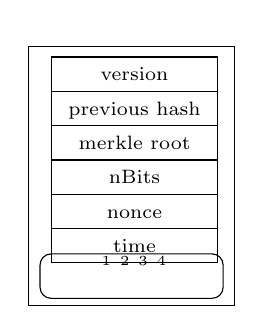
\begin{tikzpicture}[yscale=0.47,xscale=0.75]
   	\draw (0,0) rectangle (3.5,7);
   	\draw[rounded corners] (0.2,0.2) rectangle (3.3,1.4);
   	
   	\node[label,below] at(1.8,1.6) {\scriptsize $\Transaction_1$ $\Transaction_2$ $\Transaction_3$ $\Transaction_4$};
   	\node[label,below] at(1.8,7) {
	\begin{tabular}{|c|c|} \hline
              {\scriptsize \MName{version}}   		\\ \hline
	      {\scriptsize \MName{previous hash}} 	\\ \hline
              {\scriptsize \MName{merkle root}}  	\\ \hline
              {\scriptsize \MName{nBits}} 		\\ \hline
              {\scriptsize \MName{nonce}} 		\\ \hline
              {\scriptsize \MName{time}}  		\\ \hline
	\end{tabular}
	};
 
   \end{tikzpicture}
   \caption{A Bitcoin-style block containing a header and a body with transactions ($\Transaction_1$, $\Transaction_2$, $\Transaction_3$ and $\Transaction_4$).}
   \label{fig:block-structure}
\end{figure}

\section{Background: Proof-of-Work Consensus}
The {\em settlement} phase in our \DualChain{} architecture makes use of 
our novel \PoC{} protocol. The intuition behind \PoC's design stems from the 
\PoW{} protocol that helps create an immutable {\em chain of blocks}. The term 
immutable refers to the fact that each block appended to the chain requires miners 
to spend their resources. As a result, if an adversary attempts to over-write 
(or rollback) a part of the chain, it needs to create an alternate chain of all the 
desired blocks. However, to force all the honest miners to switch to this alternate 
chain, the adversary needs to compute this chain of blocks at a much faster rate 
than the original chain. This implies that the adversary needs to have much greater 
power than the honest miners. Prior works have illustrated that such an attack is 
hard to realize~\cite{bc-processing}.

Prior to running the \PoW{} protocol, each miner $\Miner \in \Miners$ needs to 
create a {\em block} of transactions. Although each miner $\Miner$ has access to the 
certificate $\Certificate$, it needs to arrange the contents of this certificate in 
the format of a block. To explain the format of a block, we follow the popular 
blockchain platform, Bitcoin, where each block includes a header and body 
(refer to Figure~\ref{fig:block-structure})~\cite{blockchain-book}. 
The header includes: 
(i) {\em version} for this block, 
(ii) {\em hash} of the previous block, 
(iii) {\em merkle root} of all transactions, 
(iv) {\em nBits}, which determines the difficulty of the puzzle, 
(v) {\em nonce}, the solution for puzzle, and 
(vi) {\em time} at which block is created once the nonce is found.

Computing Merkle root of all the transactions is trivial (refer to 
Figure~\ref{fig:merkle-tree}) and requires a miner $\Miner$ to compute a pairwise 
hash from the leaf to the root. This Merkle root helps to verify if a transaction 
was included to create the Merkle tree. However, the main challenge for a miner is 
to determine the nonce. In existing \PoW{}-based platforms, to solve the complex 
puzzle, each miner needs to calculate the {\em hash of the block} such that it 
contains a specific number of leading zero bits. For this purpose, the miners have 
to find a {\em nonce} value that yields the specific hash. This essentially makes the 
\PoW{} protocol like a {\em race} where all the miners are competing against each 
other to find the nonce. Whichever miner finds a valid nonce first, it gets the chance 
to propose the next block to be added to the chain. Hence, coming up with the correct 
number of leading zero bits in the hash is important as it sets the difficulty of 
the puzzle which simplicity controls the average time taken for each winning miner 
to propose a block. Once a miner finds the valid nonce, it can fill all the entries 
in the header, and it broadcasts the new block to all the other miners.


\begin{figure}[t]\label{ex:merkle_tree}
       \centering
       \begin{tikzpicture}[scale=0.625,transform shape]
           \node[dot] (n1) at (0, 0) {};
           \node[dot] (n2) at (4, 0) {};
           \node[dot] (n3) at (8, 0) {};
           \node[dot] (n4) at (12, 0) {};
           
           \node[below] at (n1) {$h_0 = \Digest{\Transaction_1}$};
           \node[below] at (n2) {$h_1 = \Digest{\Transaction_2}$};
           \node[below] at (n3) {$h_2 = \Digest{\Transaction_3}$};
           \node[below] at (n4) {$h_3 = \Digest{\Transaction_4}$};
   
           \node[dot] (n12) at (2, 1) {} edge[->] (n1) edge[->] (n2);
           \node[dot] (n34) at (10, 1) {} edge[->] (n3) edge[->] (n4);
   
           \node[left=7pt] at (n12) {$h_{01} = \Digest{[h_0, h_1]}$};
           \node[right=7pt] at (n34) {$h_{23} = \Digest{[h_2, h_3]}$};
   
           \node[dot] (n1234) at (6, 2) {} edge[->] (n12) edge[->] (n34);
        
           \node at (6,2.5) {$h_{0123} = \Digest{[h_{01},h_{23}]}$};
   
       \end{tikzpicture}
      	\caption{A Merkle tree over four transactions ($\Transaction_1$, $\Transaction_2$, 
      	$\Transaction_3$ and $\Transaction_4$) stored at the leaf nodes of the tree.}
	\label{fig:merkle-tree}
\end{figure} 


Notice that the ledger is essentially a chain of blocks (refer to Figure~\ref{fig:blockchain}).
In \PoW{}, it is possible that multiple miners propose the next block with valid 
nonces at approximately the same period of time. In such a case, the protocol states 
that each miner would only accept the first block it receives. This could lead to 
temporary branches or {\em forks}, all of which have the same previous hash. However, 
this condition resolves as time goes by because the protocol also expects the honest 
miners to stick to the {\em longest chain}\textemdash the one with the largest number 
of blocks. Eventually, all the shorter forks are discarded, and only the longest 
chain survives.

{\em Incentives.} 
Considering discarded forks and resources spent in the search for a valid nonce, 
what motivates a miner to participate in \PoW{} consensus? The answer is incentives. 
\PoW{}-based systems like Bitcoin reward the winning miner of the block present 
in the longest chain. These rewards help to offset the mining costs and maintain a  
sufficient number of honest miners. This requires a few more entries in the block header, 
which provide information such as the miner's account address and the reward amount.


\begin{figure}[t]
       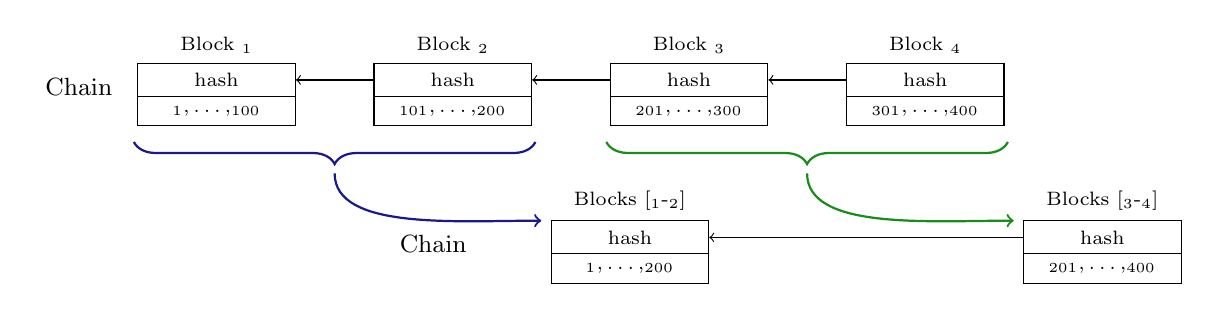
\begin{tikzpicture}[xscale=1.5,list/.style={minimum width=2cm,rectangle split, rectangle split parts=2,draw, rectangle split}]

           \node[list] (A) at (0, 0) {\scriptsize \MName{hash}\nodepart{two}\scriptsize \MName{$\Transaction_1, \dots, \Transaction_{100}$}};
           \node[list] (B) at (2, 0) {\scriptsize \MName{hash}\nodepart{two}\scriptsize \MName{$\Transaction_{101}, \dots, \Transaction_{200}$}};
           \node[list] (C) at (4, 0) {\scriptsize \MName{hash}\nodepart{two}\scriptsize \MName{$\Transaction_{201}, \dots, \Transaction_{300}$}};
           \node[list] (D) at (6, 0) {\scriptsize \MName{hash}\nodepart{two}\scriptsize \MName{$\Transaction_{301}, \dots, \Transaction_{400}$}};
           \node[above] at (A.north) {\scriptsize \MName{Block $\block_1$}};
           \node[above] at (B.north) {\scriptsize \MName{Block $\block_2$}};
           \node[above] at (C.north) {\scriptsize \MName{Block $\block_3$}};
           \node[above] at (D.north) {\scriptsize \MName{Block $\block_4$}};
           \path (D.text west) edge[->] (C.text east)
                 (C.text west) edge[->] (B.text east)
                 (B.text west) edge[->] (A.text east)
                 (A.text west);
                                         
\draw[decoration={brace,amplitude=8pt,mirror},decorate,thick,blue!50!black!90] (-0.7, -0.6) -- (2.7,-0.6);                 

\draw[decoration={brace,amplitude=8pt,mirror},decorate,thick,green!50!black!90] (3.3, -0.6) -- (6.7,-0.6);                 

\draw [->,thick, blue!50!black!90] (1,-1) to [out=270,in=180] (2.75,-1.6);
\draw [->,thick, green!50!black!90] (5,-1) to [out=270,in=180] (6.75,-1.6);
                 
                 
           \node[list] (E) at (3.5, -2) {\scriptsize \MName{hash}\nodepart{two}\scriptsize \MName{$\Transaction_{1}, \dots, \Transaction_{200}$}};
           \node[list] (F) at (7.5, -2) {\scriptsize \MName{hash}\nodepart{two}\scriptsize \MName{$\Transaction_{201}, \dots, \Transaction_{400}$}};
           \node[above] at (E.north) {\scriptsize \MName{Blocks [$\block_1$-$\block_2$]}};
           \node[above] at (F.north) {\scriptsize \MName{Blocks [$\block_3$-$\block_4$]}};
           \path (F.text west) edge[->] (E.text east);
           
\node[left] at (-0.8, 0.1) {{\small $\PBFT{}$ \MName{Chain}}};
\node[left] at (2.2, -1.9) {{\small $\PoC{}$ \MName{Chain}}};                            
                 
       \end{tikzpicture}
       \caption{A schematic representation of a blockchain or ledger in the 
       \DualChain{} architecture that consists of $\PBFT{}$ chain (i.e., \textit{layer 1}) 
       and $\PoC{}$ chain (i.e., \textit{layer 2}) that shows committed and settled 
       transactions $\Transaction_1, \dots, \Transaction_{400}$ on the $\PBFT{}$ and  
       $\PoC{}$ chains, respectively. The $i^{th}$ block holds a \emph{hash value} 
       hash$_{i-1}$ that identifies the preceding block and Block $\block_1$ is the  
       genesis block that does not have the preceding block.}
	\label{fig:blockchain}
\end{figure}



\subsection{\PoW{} Challenges}
The key issue with running the \PoW{} consensus is that it leads to massive 
waste in energy and efforts:
(1) Forks of the longest chain are subsequently discarded, which is a loss of 
resources for some miners who did find a valid nonce but did not receive any rewards.
(2) Rational miners may acquire more resources to improve their chances of proposing 
the next block, but this leads to increasing the difficulty of hash computation to 
ensure fairness.
(3) As the number of miners increases, the frequency of a single miner winning rewards 
decreases. 
(4) Several miners may work together in groups to find the valid nonce to increase 
their probability of winning rewards. This behavior significantly decreases the 
probability for a lone miner to propose the next block.
(5) Malicious miners may attempt to perform attacks like selfish mining and 
double-spending, which can rollback client transactions and invalidate the rewards earned 
by honest miners~\cite{blockchain-book}.

These issues are so prevalent in blockchain systems like Bitcoin that, 
at present, almost every miner is trying to join some existing group. In these 
groups, miners {\em pool} their resources to find a valid nonce and propose the 
next block~\cite{pooled-mining}. Every pool has its own participation rules and 
distributes rewards according to its policies. Despite this, the difficulty of hash 
computation is periodically increased or decreased in accordance with the average 
time to find a nonce by a pool of miners.

To address these challenges, in this paper, we aim to initiate a new avenue of research 
centered around hybrid consensus and collaborative mining. In particular, as a first step,
we propose our novel {\em Power-of-Collaboration} (\PoC) protocol that re-imagines 
the \PoW{} consensus.
\section{\DualChain{} Architecture}
\label{s:dual}
Our \DualChain{} runs two distinct consensus protocols in parallel. 
Specifically, it requires the replicas in set $\Replicas{}$ to commit each client transaction
through a \BFT{} consensus protocol (commitment phase), following which the miners in set $\Miners{}$ run our \PoC{} 
consensus (settlement protocol). As all the \BFT{} protocols follow the consensus dictated by 
\pbft~\cite{pbftj}, we use \pbft{} as the representative protocol 
for the ensuing discussions.
%
{\em To summarize:} each client sends its request to the replicas running the \pbft{} protocol. 
Once these replicas commit this request, they forward it to the miners. 
These miners collaboratively run the \PoC{} consensus protocol, post 
which they add a block to the ledger. Next, we discuss each of these steps 
in detail.

\begin{figure}[t]
   \centering
   \begin{tikzpicture}[yscale=0.5,xscale=0.75]
       \draw[thick,draw=black!75] (1.75,   0) edge ++(10.5, 0)
                                  (1.75,   1) edge ++(10.5, 0)
                                  (1.75,   2) edge ++(10.5, 0)
                                  (1.75,   3) edge[blue!50!black!90] ++(10.5, 0)
                                  (1.75,   4) edge[green!50!black!90] ++(10.5, 0);

       \draw[thin,draw=black!75] (2, 0) edge ++(0, 4)
                                 (4,   0) edge ++(0, 4)
                                 (6, 0) edge ++(0, 4)
                                 (8,   0) edge ++(0, 4)
                                 (10,   0) edge ++(0, 4);

       \node[left] at (1.8, 0) {\scriptsize $\Replica_3$};
       \node[left] at (1.8, 1) {\scriptsize $\Replica_2$};
       \node[left] at (1.8, 2) {\scriptsize $\Replica_1$};
       \node[left] at (1.8, 3) {\scriptsize $\Primary{}$};
       \node[left] at (1.8, 4) {\scriptsize $\Client$};

       \path[->] (2, 4) edge [red!50](4, 3)
       
                 (4, 3) edge (6, 2)
                        edge (6, 1)
                        edge (6, 0)                        
                       
                 (6, 0) edge (8, 1)
                        edge (8, 2)
                        edge (8, 3)      
                
                 (6, 1) edge (8, 0)
                        edge (8, 2)
                        edge (8, 3)
                       
                 (6, 2) edge (8, 0)
                        edge (8, 1)
                        edge (8, 3)

                 (8, 0) edge (10, 1)
                        edge (10, 2)
                        edge (10, 3)
                       
                 (8, 1) edge (10, 0)
                        edge (10, 2)
                        edge (10, 3)
                       
                 (8, 2) edge (10, 0)
                        edge (10, 1)
                        edge (10, 3)
                       
                 (8, 3) edge (10, 0)
                        edge (10, 1)
                        edge (10, 2)
                 (10, 0) edge (12, 4)
                 (10, 1) edge (12, 4)
                 (10, 2) edge (12, 4)
                 (10, 3) edge (12, 4);
      
       \node[dot,colA] at (10, 0) {};
       \node[dot,colA] at (10, 1) {};
       \node[dot,colA] at (10, 2) {};
       \node[dot,colA] at (10, 3) {};
      
       \path (10, 3) edge[thick,colA] (10, -1.3);
       %\node[label,below right,align=left] at (10, 0) {\scriptsize \MName{Inform}};

       \node[label,below,yshift=3pt] at (3, 5) {\scriptsize \MName{$\Transaction$}};
       \node[label,below,yshift=3pt] at (5, 0) {\scriptsize \MName{PrePrepare}};
       \node[label,below,yshift=3pt] at (7, 0) {\scriptsize \MName{Prepare}};
       \node[label,below,yshift=3pt] at (9, 0) {\scriptsize \MName{Commit}};
       \node[label,below,yshift=3pt] at (11, 0) {\scriptsize \MName{Inform}};
   \end{tikzpicture}
   \caption{A schematic representation of the normal-case of the \pbft{} 
   protocol with $\n{\Replicas{}} = 4$ and $\f{\Replicas} = 1$. 
	%The primary $\Primary$ proposes a transaction $\Transaction{}$ submitted by client $\Client$ to all replicas via a $\MName{PrePrepare}$ message. Next, each replica broadcasts a $\MName{Prepare}$ message for $\T$. Upon a replica $\Replica$ receives $\NonFaulty_{pbft}$ for $\T$ from distinct replicas, $\Replica$ broadcasts a $\MName{Commit}$ message. Upon a replica $\Replica$ receives $\T$ from distinct replicas, execute $\T$ and inform $\Client$ the outcome.
	}
   \label{fig:pbft}
\end{figure}


\subsection{Client Request and Transaction Ordering}
\pbft{} follows the primary-backup model where one replica is designated as the 
{\em primary} while other replicas act as backups. Each consensus is led by the 
primary replica of the current {\em view}. In the case the primary is malicious, 
{\em view-change} takes place to replace the primary. We use Figure~\ref{fig:pbft} 
to illustrate the three phases of \pbft{}.


{\em Client Request.}
A client $\Client{}$ that wants to process a transaction $\Transaction{}$ in 
our \DualChain{} architecture creates a request $\SignMessage{\Transaction}{\Client{}}$ 
and sends it to the replica designated as the primary of the view $v$. The 
client $\Client{}$ uses \DS{} to sign this message and 
adds a monotonically increasing timestamp to this message.

{\em Pre-prepare.} 
When the primary $\Primary{}$ replica receives a well-formed client request 
$m := \SignMessage{\Transaction}{\Client{}}$, it assigns $m$ a sequence number 
$k$ and creates and sends a $\MName{Preprepare}$ message to all the replicas.
This $\MName{Preprepare}$ message also includes a digest $\Hash{m}$ of $m$, 
which is used in future communication to save space. During this phase, it is 
sufficient for the primary to sign the messages using \MAC{}.
%
When a replica $\Replica{} \in \Replicas{}$ receives a well-formed 
$\MName{Preprepare}$ message from the primary $\Primary{}$ of view $v$, it agrees 
to support the order $k$ for $m$ if it has not agreed to order another request 
at sequence number $k$. The replica $\Replica$ shows its support by broadcasting 
a $\MName{Prepare}$ message.

{\em Prepare.}
When a node $\Replica{}$ receives identical $\MName{Prepare}$ messages from 
$2\f{\Replicas{}}+1$ distinct replicas (can include its own message to reach the 
count), it marks the request $m$ as {\em prepared} and broadcasts a $\MName{Commit}$ 
message. In \DualChain, we require each replica $\Replica{}$ to use $\MName{DS}$ 
to sign the $\MName{Commit}$ message.

{\em Commit.}
When $\Replica{}$ receives identical $\MName{Commit}$ messages from 
$2\f{\Replicas{}}+1$ replicas, it marks $m$ as {\em committed}. If $\Replica{}$ 
has executed all requests with sequence number less than $k$, it executes $m$ and 
sends a $\MName{Response}$ message to the client, which includes the result of 
execution $r$. The client $\Client$ marks $\SignMessage{\Transaction}{\Client{}}$ 
as processed when it receives identical $\MName{Response}$ messages from at least 
$\f{\Replicas{}}+1$ replicas.

{\bf \em Chain Communication.} 
Post consensus on $m$, each replica $\Replica$ creates a certificate $\Certificate$, 
which includes: 
(i) the client request $m$,
(ii) $\MName{Commit}$ messages for $m$ from $2\f{\Replicas{}}+1$ replicas, and
(iii) the result $r$.
Next, the replicas may follow the {\em cluster-sending} protocol~\cite{byz-cluster-sending} 
or delayed replication protocol~\cite{delayedrepl} to communicate with the miners 
in set $\Miners$.\footnote{We can model chain communication as either push- or pull-based 
model using existing peer-to-peer communication primitives.} The cluster-sending 
protocol guarantees the delivery of at least one message between the two clusters, 
given that less than one-third of members of each cluster are malicious. To do so, 
each member from the sending cluster sends a message to a distinct member in the 
receiving member. In our case, we need the certificate $\Certificate$ to be sent to 
at least $2\f{\Miners}+1$ miners: replica $\Replica{1}$ sends $\Certificate$ to miner 
$\Miner_{1}$; replica $\Replica{2}$ sends $\Certificate$ to miner $\Miner_{2}$, and 
so on.


\begin{figure}[t]
   \centering
    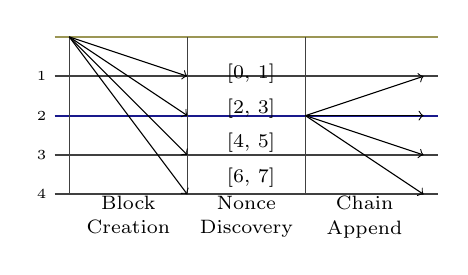
\begin{tikzpicture}[yscale=0.5,xscale=0.75]
           \draw[thick,draw=black!75] (1.75,   0) edge ++(6.5, 0)
                                   (1.75,   1) edge ++(6.5, 0)
                                   (1.75,   2) edge [blue!50!black!90] ++(6.5, 0)
                                   (1.75,   3) edge ++(6.5, 0)
                                   (1.75,   4) edge [yellow!50!black!90]++(6.5, 0);

           \node[label,below,yshift=3pt] at (3, 0) {\scriptsize \MName{Block}};
           \node[label,below,yshift=-6pt] at (3, 0) {\scriptsize \MName{Creation}};
           \node[label,below,yshift=3pt] at (5, 0) {\scriptsize \MName{Nonce}};
           \node[label,below,yshift=-6pt] at (5, 0) {\scriptsize \MName{Discovery}};
           \node[label,below,yshift=3pt] at (7, 0) {\scriptsize \MName{Chain}};
           \node[label,below,yshift=-6pt] at (7, 0) {\scriptsize \MName{Append}};
            
           \draw[thin,draw=black!75]   (2, 0) edge ++(0, 4)
                                       (4, 0) edge ++(0, 4)
                                       (6, 0) edge ++(0, 4);

           \node at (5, 1.8) {
                  \renewcommand{\arraystretch}{1.05}
           \begin{tabular}{c}
                  {\scriptsize[0, 1]}  \\
                  {\scriptsize[2, 3]}  \\
                  {\scriptsize[4, 5]}  \\
                  {\scriptsize[6, 7]}  \\
           \end{tabular}
           };

       \node[left] at (1.8, 0) {\scriptsize $\Miner_4$};
       \node[left] at (1.8, 1) {\scriptsize $\Miner_3$};
       \node[left] at (1.8, 2) {\scriptsize $\Miner_2$};
       \node[left] at (1.8, 3) {\scriptsize $\Miner_1$};
       \node[left] at (1.8, 4) {\scriptsize $\PBFT{}$};
       
       \path[->] (2, 4) 
                            edge (4, 3)                      
                            edge (4, 2)     
                            edge (4, 1)
                            edge (4, 0);
       \path[->] (6, 2) 
                            edge (8, 3)                      
                            edge (8, 2)
                            edge (8, 1)
                            edge (8, 0);

    \end{tikzpicture}
    	\caption{A schematic representation of the \PoC{} protocol with 
    	$\Miners{} = \{\Miner_1, \Miner_2, \Miner_3, \Miner_4\}$. 
    	The total solution space $\Slice{}$ is $[0,7]$ and is divided into four 
    	slices $([0,1], [2,3], [4,5], [6,7])$. Miners receive transactions from 
    	the \pbft{} replicas. Post creating a block, each Miner 
    	$\Miner_{i}$, $i \in [1,4]$ tries to discover the nonce in its slice 
    	$\Slice{i}$. Assume the valid nonce is $2$, then once $\Miner_2$ discovers 
    	the nonce, it broadcasts the same to other miners.
	}
	\label{fig:poc}
\end{figure}

When a miner $\Miner \in \Miners$ receives a certificate $\Certificate$ from 
a replica $\Replica \in \Replicas$, it broadcasts this certificate to all the 
other miners. As at least $2\f{\Miners}+1$ miners receive certificates, there 
is a guarantee that at least one honest miner will broadcast the certificate.
As a result, each miner will have access to the certificate $\Certificate$, and 
it can proceed with the \PoC{} computation.


\subsection{Collaborative Mining}
Post \pbft{} consensus, our \DualChain{} system runs the \PoC{} protocol on the 
agreed transaction to securely bind it to the ledger.
\PoC{} requires all the miners to {\em collaborate} and work together to compute 
the required hash. To do so, \PoC{} divides the \PoW{} hash computation into 
$\n{\Miners}$ disjoint subproblems and requires each miner to work on a distinct 
predetermined subproblem.

Let, $\Slice{}$ represent the solution space; all the random numbers that a miner 
has to try to find a valid nonce. Without the loss of generality, let us divide 
$\Slice{}$ into $\n{\Miners}$ equal slices, 
$\{ \Slice{1}, \Slice{2}, \cdots \Slice{\n{\Miners}} \}$, such that%

\begin{equation}
\Slice{1} \cap \Slice{2} \cap \cdots \cap \Slice{\n{\Miners}} = \varnothing 
\end{equation}%

\begin{equation}
\Slice{1} \cup \Slice{2} \cup \cdots \cup \Slice{\n{\Miners}} = \Slice{} 
\end{equation}

Our \PoC{} protocol assigns slice $\Slice{1}$ to miner $\Miner_{1}$, $\Slice{2}$ 
to $\Miner_{2}$, and $\Slice{i}$ to $\Miner_{i}$, $i \in [1,\n{\Miners}]$. The key 
assumption is that if a miner takes time $\tau$ to find a valid nonce on the solution 
space $\Slice{}$, then if all the miners are honest and follow the \PoC{} protocol, 
the time required to find the nonce should be of the order 
$\BigO{\dfrac{\tau}{\n{\Miners{}}}}$.

Further, \PoC{} protocol ensures that each honest miner gets rewarded for their 
efforts; rewards are distributed among miners. If $\Diamond$ is the reward for a 
miner to find a valid nonce in \PoW{} protocol, then in our \PoC{} protocol, each 
$i^{th}$ miner $\Miner_{i}$ receives a reward $\Diamond_i$ proportional to the size 
of its slice $\Slice{i}$.%

\begin{equation} 
    \Diamond_i = \frac{\abs{\Slice{i}}}{\abs{\Slice{}}} * \Diamond
\end{equation}

In the rest of this paper, for simplicity, we assume that all the slices have the same size.

\subsubsection{\PoC{} Protocol}
Our \PoC{} protocol works in rounds, and within each round each miner tries to find 
if a valid nonce exists in its slice of the block. In the rest of this section, we 
assume that the solution space $\Slice{}$ can be deterministically divided into 
$\n{\Miners{}}$ disjoint equal slices by each miner. For example, in Figure~\ref{fig:poc}, 
the solution space $\Slice{} = [0,7]$ is divided into $\n{\Miners{}} = 4$ slices; the 
slices are: $\Slice{1} = [0,1]$, $\Slice{2} = [2,3]$, $\Slice{3} = [4,5]$, and $\Slice{4} = [6,7]$.
Designing optimal slice distribution schemes is an interesting research avenue, which 
we consider outside the scope of this work.
%It contains two steps: obtain client transactions from $\PBFT{}$ network and mining the new block. We define the transactions in $\block_i$ mined in round i as $\TXNBlock_i$ and all $\TXNBlock_i$ are the same.

{\em Certificate Dissemination.} 
The \PoC{} protocol starts when a miner $\Miner{}$ receives a certificate $\Certificate$ 
from a replica. The miner $\Miner{}$ checks if $\Certificate$ is well-formed and 
$\Certificate$ includes signatures from $2\f{\Replicas{}}+1$ replicas; a proof that 
these replicas agreed to sequence this batch of transactions at a sequence number $k$.
If this is the case, $\Miner{}$ broadcasts this certificate to other miners.
Note: although while explaining \pbft{} we considered consensus on a single transaction, 
it can be trivially extended to a batch of transactions. This batching optimization is 
employed by all the existing \BFT{} protocols to increase their 
throughputs~\cite{pbftj,poe,rcc}.

{\em Block Creation.}
When a miner $\Miner$ has the nonce for the block ordered at sequence number $k-1$, 
it initiates the creation of a block at sequence $k$. It does so by generating a Merkle root 
of all the transactions in $k^{th}$ batch and a new block header. As each miner 
$\Miner{}$ knows there are a total of $\n{\Miners}$ miners, it creates $\n{\Miners}$ 
slices and assigns itself the $i^{th}$ slice $\Slice{i}$ in round $0$, where 
$i = \ID{\Miner{}}$.

{\em Nonce Discovery.}
We assume that each miner $\Miner{}$ knows the characteristics of the expected hash 
(the number of leading zeroes). The miner uses this information to go over all the 
possible nonces in its slice range to find a valid nonce. Once a miner $\Miner$ 
computes the correct hash, it has access to a valid nonce. The miner $\Miner$ uses 
this information to complete the block header and forwards the block to all the miners.

{\em Chain Append.}
When a miner receives a block from another miner, it first validates the nonce. If 
the nonce is valid, the miner appends this block to its local blockchain and assumes 
the \PoC{} protocol for the corresponding batch as complete.
% 
Notice that if all the miners are well-behaving, then our \PoC{} protocol requires 
only one round to find the valid nonce as the nonce is present in one of the slices.
Post discovering the nonce, each miner starts working on the next block to be added to 
the chain.

%\begin{figure}[t!]\label{ex:poc_no_solution}
%   \centering
%       \centering
%    \begin{tikzpicture}[yscale=0.5,xscale=0.75]
%           \draw[thick,draw=black!75] (0.75,   0) edge ++(14.5, 0)
%                                   (0.75,   1) edge ++(14.5, 0)
%                                   (0.75,   2) edge ++(14.5, 0)
%                                   (0.75,   3) edge ++(14.5, 0)
%                                   (0.75,   4) edge [yellow!50!black!90]++(14.5, 0);
%
%           \node[label,below,yshift=3pt] at (2, 0) {\scriptsize \MName{Block [$\block{1}$]}};
%           \node[label,below,yshift=3pt] at (4, 0) {\scriptsize \MName{Nonce}};
%           \node[label,below,yshift=-6pt] at (4, 0) {\scriptsize \MName{Discovery}};
%           \node[label,below,yshift=-15pt] at (4, 0) {\scriptsize \MName{(Timeout)}};
%           \node[label,below,yshift=3pt] at (6, 0) {\scriptsize \MName{Slice}};
%           \node[label,below,yshift=-6pt] at (6, 0) {\scriptsize \MName{Shift}};
%           \node[label,below,yshift=3pt] at (8, 0) {\scriptsize \MName{Nonce}};
%           \node[label,below,yshift=-6pt] at (8, 0) {\scriptsize \MName{Discovery}};
%           \node[label,below,yshift=-15pt] at (8, 0) {\scriptsize \MName{(Timeout)}};
%           \node[label,below,yshift=3pt] at (10, 0) {\scriptsize \MName{Block}};
%           \node[label,below,yshift=-6pt] at (10, 0) {\scriptsize \MName{[$\block{1}$, $\block{2}$]}};
%           \node[label,below,yshift=3pt] at (12, 0) {\scriptsize \MName{Nonce}};
%           \node[label,below,yshift=-6pt] at (12, 0) {\scriptsize \MName{Discovery}};
%           \node[label,below,yshift=3pt] at (14, 0) {\scriptsize \MName{Chain}};
%           \node[label,below,yshift=-6pt] at (14, 0) {\scriptsize \MName{Update}};
%            
%           \draw[thin,draw=black!75]   (1, 0) edge ++(0, 4)
%                                       (3, 0) edge ++(0, 4)
%                                       (5, 0) edge ++(0, 4)
%                                       (7, 0) edge ++(0, 4)
%                                       (9, 0) edge ++(0, 4)
%                                       (11, 0) edge ++(0, 4)
%                                       (13, 0) edge ++(0, 4.2);
%
%       \node[left] at (0.8, 0) {\scriptsize $\Miner_4$};
%       \node[left] at (0.8, 1) {\scriptsize $\Miner_3$};
%       \node[left] at (0.8, 2) {\scriptsize $\Miner_2$};
%       \node[left] at (0.8, 3) {\scriptsize $\Miner_1$};
%       \node[left] at (0.8, 4) {\scriptsize $\PBFT{}$};
%
%       \node at (4, 1.8) {
%                  \renewcommand{\arraystretch}{1.05}
%           \begin{tabular}{c}
%                  {\scriptsize \MName[0, 1]}  \\
%                  {\scriptsize \MName[2, 3]}  \\
%                  {\scriptsize \MName[4, 5]}  \\
%                  {\scriptsize \MName[6, 7]}  \\
%           \end{tabular}
%           };
%
%       \path[->] (1, 4) 
%                            edge (3, 3)                      
%                            edge (3, 2)     
%                            edge (3, 1)
%                            edge (3, 0);
%       \path[->] (5, 3) 
%                            edge (7, 3)                      
%                            edge (7, 2)     
%                            edge (7, 1)
%                            edge (7, 0);
%       \path[->] (5, 2) 
%                            edge (7, 3)                      
%                            edge (7, 2)     
%                            edge (7, 1)
%                            edge (7, 0);
%       \path[->] (5, 1) 
%                            edge (7, 3)                      
%                            edge (7, 2)     
%                            edge (7, 1)
%                            edge (7, 0);
%       \path[->] (5, 0) 
%                            edge (7, 3)                      
%                            edge (7, 2)     
%                            edge (7, 1)
%                            edge (7, 0);
%       \node at (8, 1.8) {
%                  \renewcommand{\arraystretch}{1.05}
%           \begin{tabular}{c}
%                  {\scriptsize \MName[2, 3]}  \\
%                  {\scriptsize \MName[4, 5]}  \\
%                  {\scriptsize \MName[6, 7]}  \\
%                  {\scriptsize \MName[0, 1]}  \\
%           \end{tabular}
%       };
%       \path[->] (9, 4) 
%                            edge (11, 3)                      
%                            edge (11, 2)     
%                            edge (11, 1)
%                            edge (11, 0);
%       \node at (12, 1.8) {
%                  \renewcommand{\arraystretch}{1.05}
%           \begin{tabular}{c}
%                  {\scriptsize \MName[0, 1]}  \\
%                  {\scriptsize \MName[2, 3]}  \\
%                  {\scriptsize \MName[4, 5]}  \\
%                  {\scriptsize \MName[6, 7]}  \\
%           \end{tabular}
%           };
%
%       \path[->] (13, 1) 
%                            edge (15, 3)                      
%                            edge (15, 2)     
%                            edge (15, 1)
%                            edge (15, 0);
%
%    \end{tikzpicture}
%    	\caption{An example that no valid nonce can be found for the new block. If the {\em timer} $\delta$ fires because no valid new block arrives,
%           a Slice Shifting will be triggered by sending a shift message <SHIFT, h, $\ShiftRound{i}$> to other miners. If a miner $\Miner{j}$ receives
%           $2\f{\Replicas}+1$ same shift messages from distinct miners, it starts its $\ShiftRound{i+1}$ by assigning its $\Slice{j}$ to $\Slice{j+1}$
%           and start to find the valid nonce in the new $\Slice{j}$. If no valid block has been found after $\f{\Miners{}}$ rounds, we can determine 
%           that there is no solution for this new block. The transactions $\Transaction{}$ in this block will be merged into the next block and skip the
%           current one. We assume nonce 3 is the valid value for the second block that contains $\block{1} and \block{2}$ in this example.
%           }
%\end{figure}\label{fig:poc_no_solution}

\begin{figure}
   \centering
    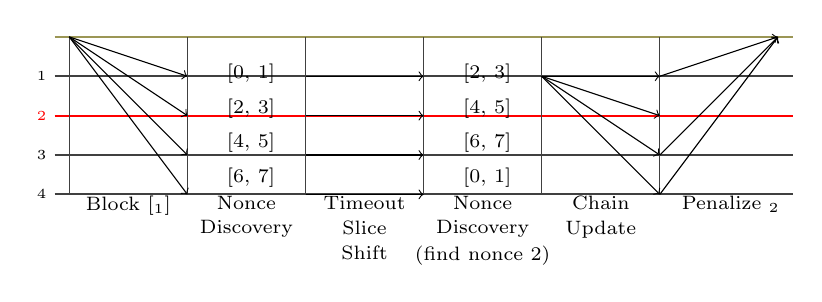
\begin{tikzpicture}[yscale=0.5,xscale=0.75]
           \draw[thick,draw=black!75] (0.75,   0) edge ++(12.5, 0)
                                   (0.75,   1) edge ++(12.5, 0)
                                   (0.75,   2) edge [red] ++(12.5, 0)
                                   (0.75,   3) edge ++(12.5, 0)
                                   (0.75,   4) edge [yellow!50!black!90]++(12.5, 0);

           \node[label,below,yshift=3pt] at (2, 0) {\scriptsize \MName{Block [$\block_{1}$]}};
           \node[label,below,yshift=3pt] at (4, 0) {\scriptsize \MName{Nonce}};
           \node[label,below,yshift=-6pt] at (4, 0) {\scriptsize \MName{Discovery}};
           \node[label,below,yshift=3pt] at (6, 0) {\scriptsize \MName{Timeout}};
           \node[label,below,yshift=-6pt] at (6, 0) {\scriptsize \MName{Slice}};
           \node[label,below,yshift=-15pt] at (6, 0) {\scriptsize \MName{Shift}};
           \node[label,below,yshift=3pt] at (8, 0) {\scriptsize \MName{Nonce}};
           \node[label,below,yshift=-6pt] at (8, 0) {\scriptsize \MName{Discovery}};
           \node[label,below,yshift=-15pt] at (8, 0) {\scriptsize \MName{(find nonce 2)}};
           \node[label,below,yshift=3pt] at (10, 0) {\scriptsize \MName{Chain}};
           \node[label,below,yshift=-6pt] at (10, 0) {\scriptsize \MName{Update}};
           \node[label,below,yshift=3pt] at (12.2, 0) {\scriptsize \MName{Penalize $\Miner_{2}$}};
            
           \draw[thin,draw=black!75]   (1, 0) edge ++(0, 4)
                                       (3, 0) edge ++(0, 4)
                                       (5, 0) edge ++(0, 4)
                                       (7, 0) edge ++(0, 4)
                                       (9, 0) edge ++(0, 4)
                                       (11, 0) edge ++(0, 4);
       \node[left] at (0.8, 0) {\scriptsize $\Miner_4$};
       \node[left] at (0.8, 1) {\scriptsize $\Miner_3$};
       \node[left,red] at (0.8, 2) {\scriptsize $\Miner_2$};
       \node[left] at (0.8, 3) {\scriptsize $\Miner_1$};
       \node[left] at (0.8, 4) {\scriptsize $\PBFT{}$};

       \node at (4, 1.8) {
                  \renewcommand{\arraystretch}{1.05}
           \begin{tabular}{c}
                  {\scriptsize \MName[0, 1]}  \\
                  {\scriptsize \MName[2, 3]}  \\
                  {\scriptsize \MName[4, 5]}  \\
                  {\scriptsize \MName[6, 7]}  \\
           \end{tabular}
           };

       \path[->] (1, 4) 
                            edge (3, 3)                      
                            edge (3, 2)     
                            edge (3, 1)
                            edge (3, 0);
       \path[->] (5, 3) 
                            edge (7, 3);
                            %edge (7, 2)     
                            %edge (7, 1)
                            %edge (7, 0);
       \path[->] (5, 2) 
                            %edge (7, 3)                      
                            edge (7, 2);     
                            %edge (7, 1)
                            %edge (7, 0);
       \path[->] (5, 1) 
                            %edge (7, 3)                      
                            %edge (7, 2)     
                            edge (7, 1);
                            %edge (7, 0);
       \path[->] (5, 0) 
                            %edge (7, 3)                      
                            %edge (7, 2)     
                            %edge (7, 1)
                            edge (7, 0);
       \node at (8, 1.8) {
                  \renewcommand{\arraystretch}{1.05}
           \begin{tabular}{c}
                  {\scriptsize \MName[2, 3]}  \\
                  {\scriptsize \MName[4, 5]}  \\
                  {\scriptsize \MName[6, 7]}  \\
                  {\scriptsize \MName[0, 1]}  \\
           \end{tabular}
       };
       \path[->] (9, 3) 
                            edge (11, 3)                      
                            edge (11, 2)     
                            edge (11, 1)
                            edge (11, 0);
       \path[->] (11, 3) 
                            edge (13, 4);
       \path[->] (11, 1) 
                            edge (13, 4);
       \path[->] (11, 0) 
                            edge (13, 4);

    \end{tikzpicture}
      \caption{An illustration of the slice shifting procedure. Here, we assume 
      $2$ is the valid nonce of the block, and the miner $\Miner_2$ is malicious. 
      Hence, $\Miner_2$ does not broadcast the block to other miners, which 
      triggers slice shifting procedure. Post slice shifting, $\Miner_1$ discovers 
      the nonce and broadcasts to other miners.
      }
	\label{fig:poc_malicious}
\end{figure}


\subsubsection{Slice Shifting Protocol}
In our \DualChain{} system, each miner receives certificates from the \pbft{} 
replicas. These certificates include client transactions that have been 
ordered by at least $2\f{\Replicas}+1$ replicas. Our \DualChain{} architecture 
uses the \PoC{} protocol to add these transactions to the ledger in the order 
defined by \pbft{} replicas. As a result, a malicious miner has limited attack 
opportunities; if a malicious miner finds a valid nonce in its slice, it can 
avoid forwarding this information to the honest miners. If such is the case, 
despite searching over its slice, each honest miner would not find any possible 
solution and would not be able to make progress.

To resolve this attack, our \PoC{} protocol requires each miner to set a 
{\em timer} $\delta$. Each miner $\Miner{}$ starts a timer $\delta$ when it 
receives a certificate from the \pbft{} replicas. $\Miner{}$ stops $\delta$ 
if it discovers the valid nonce or it receives a valid block from another miner.
If $\Miner{}$'s timer $\delta$ expires, and it does not have access to the valid 
nonce, it initiates the {\em slice shifting} protocol. Once the slice shifting 
is endorsed by the majority of miners, then each miner searches for the nonce 
in the next slice. Specifically, if prior to slice shifting a miner $\Miner{}$ 
was working on the $i^{th}$ slice $\Slice{i}$, post slice shifting $\Miner{}$ will 
work on $((i+1) \mod \n{\Miners{}})^{th}$ slice, $\Slice{(i+1)}$. As each miner 
already has access to all the slices, this switch does not require any 
additional communication.

The key intuition behind the slice shifting procedure is that even if a malicious 
miner decides to hide the nonce, post switch, it will be discovered by another miner.
However, it is possible that up to $\f{\Miners{}}$ consecutive miners may be malicious. 
As a result, the honest miners will discover the valid nonce after $\f{\Miners{}}$ shifts.%
\footnote{
The search space can be salted deterministically upon shifting to expand the search 
space and guard against rare cases in which the original problem may have no solution irrespective of minors' behavior.
}

%We impose all the solutions of $\PoW{}$ puzzles to be resolved in time T. (It is easy to restrict the solution time by modifying the difficulty, like Bitcoin estimate each block will be created average in 15 minutes and the longest mining time is no large than 2 hours from the median mining time of the previous 11 blocks[???]). 


\subsubsection{Reward and Penalty Economy}
Frequent slice shifting due to malicious miners will be detrimental to the 
performance of our \PoC{} protocol; it forces honest miners to do more work and 
wastes their resources. Moreover, why would any rational miner want to join the 
\PoC{} network and invest its computational resources? To make \PoC{} protocol 
fruitful, we incentivize all the honest miners for their efforts; all miners 
are assumed honest until proven guilty. 

First, like existing blockchain systems, such as Bitcoin and Ethereum, one of 
the aims of our \DualChain{} system is to establish a decentralized economy. 
To do so, like Bitcoin, in \PoC{}, when a miner discovers a nonce and broadcasts 
the valid block to other miners, we assume the creation of a {\em new token}. For 
brevity, we skip diving into the crypto-economics of the token generation and 
disbursement, and refer to the existing literature on the same~\cite{bitcoin,ether}. 
However, the key goal is that this token is equally divided among the honest 
miners. Further, like Bitcoin and Ethereum, we expect each client to pay some 
fees for getting its transaction processed by our \DualChain{} system. This 
fees is also equally divided among all the miners working on the current block.

To disburse transaction fees and tokens among the miners, there are two possible 
approaches: 
(i) Like Bitcoin, each miner includes $\n{\Miners{}}$ transactions that assigns an 
equal fraction of the reward to every other miner's public-key (account). These 
transactions can be deterministically created by each miner prior to mining and are 
included while creating the Merkle root. However, this will create unnecessary 
book-keeping, increasing the size of blocks.
(ii) We assume that the genesis block of the ledger records 
the information about the founding miners and their respective initial slices.
Further, miners can redistribute, resale, and divide their slices to other miners 
(similar to buying and selling of stocks), and any such transactions must be stored 
on the ledger before becoming effective. Assume that when a miner purchases a slice, 
sufficient tokens are reserved to enable penalization of misbehaving miners, 
which results in slashing their reserve funds similar to Proof-of-Stake 
designs~\cite{blockchain-book}. Given all this information, when a block is 
formed by the \PoC{} miners, we add the incentives to the accounts of
the respective miners; miners can validate if they received incentives or not. 

This rewarding process of \PoC{} is similar to strategies adopted by 
{\em mining pools} in systems like Bitcoin. Most importantly, in \PoC{}, the 
agreement on what to be included in the next block is strictly determined by \PBFT{} 
chain, not miners. This substantially simplifies the design of \PoC{} by making it 
deterministic, eliminating any lottery-based or leader-less consensus challenges 
that traditional \PoW{} must cope with. Furthermore, we present the novel idea of 
slice shifting for the cases when no miner in a round broadcasts a valid nonce. 
As slice shifting requires each miner to work on the next slice to find the nonce, 
it is expensive. We mitigate the need for slice shifting by heavily {\em penalizing} 
malicious miners. Specifically, we require each miner to count the number of 
{\em shifts} it took to find a valid nonce and to identify the miner who failed 
to find the valid nonce. Further, as the order of all initial slice assignments is known 
to all the miners, so each miner can trivially determine which miner was responsible 
for previous shifts. Notice that any misbehaving miner will be discovered and penalized 
as it diminishes the returns for other honest miners. 


%\begin{lemma}
%    If a non-faulty miner finds out the solution and broadcasts the new block in the ShiftRound $\ShiftRound{i}$, at least $2*\f{\Miners{}}+1$ miners will receive 
%    the new block in $\ShiftRound{i}$ if the following assumptions are ture [...].
%\end{lemma}


%We use pay-per-share(PPS)[???] as a reward stratery. Whenever a new block is created, every miner will receive the reward 
%according to their exploring solution space ($\Slice$). 
%


%Once a miner receives a new block in its shift round $\ShiftRound_i$, it believes that the solution owners on $[\ShiftRound_1 \cdots \ShiftRound_{i-1}$ are faulty 
%and should be punished, by sneding a new message <PENALIZE, Miners, height> via $\PBFT{}$ network where Miners are the faluty 
%minters who did not work on the solution in the previous shift round, heigh is the current block height. Once a replica in $\PBFT{}$ network
%receives $2*F^{\PoW{}}+1$ same penalty messages from different miners, send a <PENALIZE\_ACK,Miners,height> to the current primary.
%Once the current primary receives $2*F^{\PBFT{}}+1$ PENALIZE\_ACK messages from distinct replicas, submit the PENALIZE\_ACK message via a
%new transaction by $\PBFT{}$ consensus algorithm. This transaction will be executed by all the miners eventually thought $\PoC$ protocol.
%(Figure $\ref{fig:penalty_normal_case}$)
%
%If a replica in $\PBFT{}$ network sends out a PUSHNISH\_ACK to the primary but does not receive the commit message in some timeouts, it will re-send
%the messages. If the committed message still does not arrive after some retry, it will trigger a ViewChange to change the current primary 
%(Figure $\ref{fig:penalty_timeout}$). 
%
%\input{punishment_nc}

\section{Proof-of-Concept Evaluation}
We now present an initial evaluation of our vision of \DualChain{} architecture,
which we implement in the open-sourced \ResDB{} fabric~\cite{poe,geobft,rcc, 
ringbft}.\footnote{For our proof-of-concept of \DualChain{} 
architecture, we employ an experimental version of \ResDB{} with the codename of {\em NexRes} 
(Next Generation \ResDB{}); this is an architectural rewrite of the \ResDB{} 3.0 
(the latest stable version).}

\begin{figure*}
    \centering
    \setlength{\tabcolsep}{1pt}
    \begin{tabular}{cc@{\quad}cc}
        \pbfttput&
        \pbftlat\\
    \end{tabular}
    \vspace{-3mm}
    \caption{Evaluating peak throughput and commitment latency attained by \pbft{} consensus in \DualChain{}.}
    \vspace{-3mm}
    \label{fig:performance_pbft}
\end{figure*}

\begin{figure*}
    \centering
    \setlength{\tabcolsep}{1pt}
    \begin{tabular}{cc@{\quad}cc}
        \EvalBatchTput{(a)}&
        \EvalBatchLatency{(b)}&
        \EvalMinerTput{(c)}&
        \EvalMinerLatency{(d)}\\
    \end{tabular}
    \vspace{-3mm}
    \caption{Evaluating \PoC{} throughput and average settlement latency with 
    different difficulty (D), miners (M) and block batch size (B).}
    \vspace{-3mm}
    \label{fig:performance_poc}
\end{figure*}

{\bf Experimental Setup.}
We use Oracle Cloud Infrastructure's VM.Standard2.8 architecture to deploy miners 
and replicas ($16$ cores, \SI{8.2}{Gbps} bandwidth, $120$ GB Memory). In our 
experiments, we generate $400$ million client requests of size \SI{64}{B} each,
while client response has size \SI{17}{B}. We average results over three runs.
We require clients to sign their messages using \texttt{ED25519} while replicas use 
\texttt{CMAC}.

{\bf Batching.}
We employ the standard practice of batching client transactions, which we refer to 
\textit{transaction batching}, to optimize the \pbft{} consensus. Additionally, during 
the \PoC{} consensus, each miner aggregates multiple batches from \pbft{} consensus, '
which we refer to \textit{block batching}, prior to mining. 

 
{\bf \pbft{} Scaling.}
In Figure~\ref{fig:performance_pbft}, we gauge the peak throughput and 
\textit{commitment latency} incurred by the \pbft{} consensus of our \DualChain{} 
architecture. This is an important metric as it informs the rate at which we 
can reply to the clients. For this experiment, we increase the number of replicas 
from $16$ to $120$ and require the primary to process a batch of $100$ 
transactions per consensus; transaction batch size is set to $100$. 
As expected, on increasing the number of replicas, there is a drop in peak 
throughput and an increase in incurred latency, which remains in the subsecond 
range. This phenomenon occurs because, at each setting, we are approximately 
hitting the network bandwidth; as the number of replicas increases, more messages 
are communicated per consensus. In summary, the peak throughput reaches well 
over \SI{800}{k} transactions/second at $16$ replicas while sustaining over 
\SI{100}{k} transactions/second even when scaling to as many as $120$ replicas.


{\bf \PoC{} Scaling.}
Next, we study the impact of our \PoC{} consensus protocol on the \DualChain{} 
architecture. We deploy $120$ replicas for running \PBFT{} consensus. For the 
\PoC{} setting, we set the solution space parameter to $42$ nonce bits and 
split it into equal disjoint slices based on the number of miners. Notice that 
the difficulty of each problem is the number of leading zeros in the hash. In 
Figure~\ref{fig:performance_poc}, we present our results; here $D$ refers to 
difficulty (with the default of $D=9$), $M$ refers to the number of miners 
(with the default of $M=120$), and $B$ refers to the number of batches in a block. 
As stated earlier, for every $B$ blocks produced by \PBFT{} a single block is 
notarized and minted by \PoC{}.
 
In Figures~\ref{fig:performance_poc}(a) and~\ref{fig:performance_poc}(b), 
we fix the number of miners to $120$, which allows creating $120$ equal slices, and 
increase the block size from \SI{120}{k} to \SI{280}{k}. We test at two 
difficulty levels: $D=8$ and $D=9$. Our results indicate that $D=8$ is 
relatively easy, due to which each miner has to perform a smaller amount 
of work. As a result, any increase in batch size does not increase peak 
throughput. Hence, we test on $D=9$ at which mining smaller batch size 
impacts the system throughput as miners have to participate in a larger 
number of consensus rounds. On further increasing the block size, 
we observe that the throughput hits the \PBFT{}'s peak as desired. Thus, 
notarizing the blocks by \PoC{} no longer hinders the system throughput, 
it only prolongs the \textit{settlement latency} as expected. 
%
When examining the end-to-end system throughput of \DualChain{} which 
includes both \PBFT{} and \PoC{}, we observe a sustained throughput 
of \SI{105}{k} with a commitment latency of $1$ second and the settlement 
latency of $198$ seconds when the batch size is set to \SI{200}{k}. 
{\em Note:} We could not test at difficulty beyond $D=9$ as each nonce 
computation became prohibitively time- and resource-intensive given 
our available commodity hardware.

In Figures~\ref{fig:performance_poc}(c) and~\ref{fig:performance_poc}(d), 
we gauge the performance of \PoC{} when there are $64$ to $120$ miners. 
For these experiments, we also test at three different block batch sizes. 
As expected, the degree of collaborative mining is directly proportional 
to the number of miners. As we increase the number of miners, there is an
increase in peak throughput and a decrease in the settlement latency.


%In our experiments, we realize \mo{as expected not we realized} that when 
%the mining time is always smaller than the transaction producing time, 
%the miners will be always waiting for the transactions before they start 
%the \PoW{}. In this case, the \PoW{} throughput will be the same as the 
%\PBFT{} throughput. For example, it is much easier to find out the 
%solutions when we set the difficulty as eight. When we set up BBS larger 
%than 80K which will need 1.5 minute to fulfill in our \PBFT{} setting 
%but the mining latency is less than 1.5 minutes, the miners are idle 
%at most of the time. The throughput is consistence.  Thus, the throughput 
%will always be around (see  $\ref{fig:performance_poc}$). We also found 
%when we increase BBS to 120K, the throughput for difficulty nine will 
%also be around 100k. Due to the limitation of computation resource, 
%we are not able to evaluate the performance of difficulty ten.
%
%\mo{add the precise stats that justify our choice, for example, on 
%average solving puzzle with 9 leading zeros requires 3.724789943 minutes with 
%2 minutes standard deviation, which is why this block range make 
%sense} 
 

%\mo{for caption text, please see our earlier paper for more standard 
%formats.}

%\section{Related Work}
\label{sec:related-work}
\noindent \textbf{Pseudo-relevance feedback:} Our method has similarities with %the existing approach of 
Pseudo-Relevance Feedback (PRF) \cite{rocchio1971relevance, lv2009adaptive, li2022does} in IR: \cite{bendersky2011parameterized, xu2017quary} use the retrieved documents to improve sparse approaches via query expansion or query term reweighting, \cite{li2018nprf, zheng2020bert} score similarity between a target document and a top-ranked feedback document, while \cite{yu2021improving} train a separate query encoder that computes a new query embedding using the retrieved documents as additional input. In contrast, our approach does not require customized training feedback models or availability of explicit feedback data, as we improve the query vector by directly distilling from the reranker's output within an R\&R framework. %\pradeep{Why is our approach better?} 

Further, previous approaches to PRF have been dependent on the choice of retriever architecture and language; \cite{yu2021improving}'s PRF model is tied to the retriever used, \cite{chandradevan2022learning} explore cross-lingual relevance feedback, but require feedback documents in target language and thereby could only apply to three languages, while \cite{li2022interpolate} explore interpolating relevance feedback between dense and sparse approaches.
On the other hand, our approach is independent of the choice of the retriever and reranker architecture, and can be used for neural retrieval in any domain, language or modality. \\

\noindent \textbf{Distillation in Neural IR:} Existing approaches primarily leverage reranker feedback \textit{during training} of the dual-encoder retriever, to sample better negatives \cite{qu2021rocketqa}, for standard knowledge distillation of the cross-attention scores \cite{izacard2020distilling}, to train smaller and more efficient rankers by distilling larger models \cite{hofstatter2020improving}, or to align the geometry of dual-encoder embeddings with that from cross-encoders \cite{wang2021enhancing}. Instead, we leverage distillation at inference time, updating only the query representation to replicate the cross-encoder’s scores for the corresponding test instance.
A key implication of this design choice is that unlike existing methods, we keep the retriever parameters unchanged, meaning \textsc{ReFIT} can be incorporated out-of-the-box into any neural R\&R framework. In contrast, extending training-time distillation to new languages or modalities would require re-training the bi-encoder.

More recently, \textsc{TouR}~\cite{sung2023optimizing} has proposed test-time optimization of query representations with two variants: \textsc{TouR}$_{\text{hard}}$ and  \textsc{TouR}$_{\text{soft}}$. 
\textsc{TouR}$_{\text{hard}}$ optimizes the marginal likelihood of a small set of (pseudo) positive contexts.
\textsc{ReFIT} shares similarities with \textsc{TouR}$_{\text{soft}}$, which uses the normalized scores of a cross-encoder over the retrieved results as soft labels.
Crucially, \textsc{TouR} relies on multiple iterations of relevance feedback via distillation, where each iteration runs until the top-1 retrieval result has the highest reranker score (in \textsc{TouR}$_{\text{soft}}$) or is a pseudo-positive (in \textsc{TouR}$_{\text{hard}}$).
This makes inference highly computationally expensive, as each additional iteration involves labeling top-$K$ retrieval results with a reranker and then retrieving again.
\textsc{ReFIT} improves efficiency over \textsc{TouR} by requiring only a single iteration of feedback that simply updates the query vector for longer, foregoing additional retrieval and reranking steps. More specifics on the inference process of the two methods can be found in \S{\ref{sec:tour_comparison}}.
\textsc{TouR} was evaluated only on English phrase and passage retrieval tasks, while we demonstrate \textsc{ReFIT}'s effectiveness in multidomain, multilingual and multimodal settings, with an empirical comparison with \textsc{TouR} in \S{\ref{sec:tour_comparison}}.
\section{Conclusions}
In this paper, we present the vision of our \DualChain{} system, which facilitates 
the creation of a safe and efficient decentralized economy. \DualChain{} achieves these 
guarantees by separating the life-cycle of a client transaction into two phases: 
commitment and settlement. In the commitment phase, \DualChain{} employs a 
traditional \BFT{} protocol to order the client transactions. Post this, \DualChain{} 
requires a set of miners to run the settlement phase, where they notarize the ordered 
client transactions. Our \DualChain{} architecture does not impact the transaction 
latency observed by the client as each client receives the commitment response post 
\BFT{} consensus. Further, to efficiently notarize transactions during the settlement 
phase, our \DualChain{} architecture introduces the notion of collaborative mining, 
where participants work together instead of competing with each other. These notarized 
transactions are written to a ledger and can be queried in the future.


\section{Acknowledgments}
This work was supported in part by (1) {\em Oracle Cloud Credits} and 
related resources provided by the Oracle for Research program and (2) the 
{\em NSF STTR} under {\em Award Number} 2112345 provided to {\em Moka Blox LLC}.


%\balance
%\bibliographystyle{plain}
%\bibliography{submissions/junchao/refined}

\begin{thebibliography}{10}

\bibitem{sharper}
Mohammad~Javad Amiri, Divyakant Agrawal, and Amr El~Abbadi.
\newblock {\em {SharPer: Sharding Permissioned Blockchains Over Network
  Clusters}}, page 76–88.
\newblock Association for Computing Machinery, 2021.

\bibitem{bedrock}
Mohammad~Javad Amiri, Chenyuan Wu, Divyakant Agrawal, Amr~El Abbadi, Boon~Thau
  Loo, and Mohammad Sadoghi.
\newblock The bedrock of {BFT:} {A} unified platform for {BFT} protocol design
  and implementation.
\newblock {\em CoRR}, abs/2205.04534, 2022.

\bibitem{pbftj}
Miguel Castro and Barbara Liskov.
\newblock Practical byzantine fault tolerance and proactive recovery.
\newblock {\em ACM Trans. Comput. Syst.}, 20(4):398--461, 2002.

\bibitem{ahl}
Hung Dang, Tien Tuan~Anh Dinh, Dumitrel Loghin, Ee-Chien Chang, Qian Lin, and
  Beng~Chin Ooi.
\newblock Towards scaling blockchain systems via sharding.
\newblock In {\em Proceedings of the 2019 International Conference on
  Management of Data}, pages 123--140. ACM, 2019.

\bibitem{badcoin}
Alex de~Vries.
\newblock Bitcoin's growing energy problem.
\newblock {\em Joule}, 2(5):801--805, 2018.

\bibitem{sybil-attack}
John~R. Douceur.
\newblock The sybil attack.
\newblock In Peter Druschel, Frans Kaashoek, and Antony Rowstron, editors, {\em
  Peer-to-Peer Systems}, pages 251--260, Berlin, Heidelberg, 2002. Springer
  Berlin Heidelberg.

\bibitem{poe}
Suyash Gupta, Jelle Hellings, Sajjad Rahnama, and Mohammad Sadoghi.
\newblock {Proof-of-Execution}: Reaching consensus through fault-tolerant
  speculation.
\newblock In {\em Proceedings of the 24th International Conference on Extending
  Database Technology}, 2021.

\bibitem{blockchain-book}
Suyash Gupta, Jelle Hellings, and Mohammad Sadoghi.
\newblock {\em {Fault-Tolerant Distributed Transactions on Blockchain}}.
\newblock Synthesis Lectures on Data Management. Morgan {\&} Claypool
  Publishers, 2021.

\bibitem{rcc}
Suyash Gupta, Jelle Hellings, and Mohammad Sadoghi.
\newblock {RCC:} resilient concurrent consensus for high-throughput secure
  transaction processing.
\newblock In {\em 37th {IEEE} International Conference on Data Engineering,
  {ICDE} 2021, Chania, Greece, April 19-22, 2021}, pages 1392--1403. {IEEE},
  2021.

\bibitem{geobft}
Suyash Gupta, Sajjad Rahnama, Jelle Hellings, and Mohammad Sadoghi.
\newblock {ResilientDB}: Global scale resilient blockchain fabric.
\newblock {\em Proc. VLDB Endow.}, 13(6):868--883, 2020.

\bibitem{flexitrust}
Suyash Gupta, Sajjad Rahnama, Shubham Pandey, Natacha Crooks, and Mohammad
  Sadoghi.
\newblock Dissecting {BFT} consensus: In trusted components we trust!
\newblock {\em CoRR}, abs/2202.01354, 2022.

\bibitem{bc-processing}
Suyash Gupta and Mohammad Sadoghi.
\newblock Blockchain transaction processing.
\newblock In {\em Encyclopedia of Big Data Technologies}, pages 1--11.
  Springer, 2019.

\bibitem{byz-cluster-sending}
Jelle Hellings and Mohammad Sadoghi.
\newblock Brief announcement: The fault-tolerant cluster-sending problem.
\newblock In Jukka Suomela, editor, {\em 33rd International Symposium on
  Distributed Computing, {DISC} 2019}, volume 146 of {\em LIPIcs}, pages
  45:1--45:3, 2019.

\bibitem{delayedrepl}
Jelle Hellings and Mohammad Sadoghi.
\newblock Coordination-free byzantine replication with minimal communication
  costs.
\newblock In {\em 23rd International Conference on Database Theory, {ICDT}},
  pages 17:1--17:20, 2020.

\bibitem{cryptobook}
Jonathan Katz and Yehuda Lindell.
\newblock {\em Introduction to Modern Cryptography}.
\newblock Chapman and Hall/CRC, 2nd edition, 2014.

\bibitem{bitcoin}
Satoshi Nakamoto.
\newblock Bitcoin: A peer-to-peer electronic cash system, 2009.

\bibitem{ringbft}
Sajjad Rahnama, Suyash Gupta, Rohan Sogani, Dhruv Krishnan, and Mohammad
  Sadoghi.
\newblock {RingBFT: Resilient Consensus over Sharded Ring Topology}.
\newblock In {\em Proceedings of the 25th International Conference on Extending
  Database Technology}, pages 2:298--2:311. OpenProceedings.org, 2022.

\bibitem{pooled-mining}
Meni Rosenfeld.
\newblock Analysis of {Bitcoin} pooled mining reward systems, 2011.

\bibitem{mirbft}
Chrysoula Stathakopoulou, Matej Pavlovic, and Marko Vukolic.
\newblock State machine replication scalability made simple.
\newblock In Y{\'{e}}rom{-}David Bromberg, Anne{-}Marie Kermarrec, and Christos
  Kozyrakis, editors, {\em EuroSys '22: Seventeenth European Conference on
  Computer Systems}, pages 17--33. {ACM}, 2022.

\bibitem{basil}
Florian Suri-Payer, Matthew Burke, Zheng Wang, Yunhao Zhang, Lorenzo Alvisi,
  and Natacha Crooks.
\newblock Basil: Breaking up bft with acid (transactions).
\newblock In {\em Proceedings of the ACM SIGOPS 28th Symposium on Operating
  Systems Principles}, SOSP '21, page 1–17. Association for Computing
  Machinery, 2021.

\bibitem{badbadcoin}
Harald Vranken.
\newblock Sustainability of bitcoin and blockchains.
\newblock {\em Current Opinion in Environmental Sustainability}, 28:1--9, 2017.

\bibitem{ether}
Gavin Wood.
\newblock {Ethereum: A secure decentralised generalised transaction ledger}.
\newblock 2015.

\bibitem{hotstuff}
Maofan Yin, Dahlia Malkhi, Michael~K. Reiter, Guy~Golan Gueta, and Ittai
  Abraham.
\newblock {HotStuff}: {BFT} consensus with linearity and responsiveness.
\newblock In {\em Proceedings of the ACM Symposium on Principles of Distributed
  Computing}, pages 347--356. ACM, 2019.

\bibitem{scalable-ledger}
Kaiwen Zhang and Hans-Arno Jacobsen.
\newblock Towards dependable, scalable, and pervasive distributed ledgers with
  blockchains.
\newblock In {\em 2018 IEEE 38th International Conference on Distributed
  Computing Systems (ICDCS)}, pages 1337--1346, 2018.

\end{thebibliography}

\end{document}





\end{article}

\makeatletter
\renewcommand{\AB@affillist}{}
\renewcommand{\AB@authlist}{}
\setcounter{authors}{0}
\makeatother


\begin{article}
{Transparent Sharding}
{Deepal Tennakoon, Vincent Gramoli}
\graphicspath{{submissions/tennakoon/}}
% link to instruction: https://tc.computer.org/tcde/tcde-bulletin-author-instructions/
% \documentclass[11pt,dvipdfm]{article}
\documentclass[11pt]{article}
\usepackage{tabularx}
\usepackage{ragged2e}  % for '\RaggedRight' macro (allows hyphenation)
\usepackage{booktabs}  % for \toprule, \midrule, and \bottomrule macros
\usepackage{textcomp}
\usepackage{amsfonts,amsmath}
\usepackage{deauthor,times}
\usepackage{graphicx} % 
\usepackage{hyperref}
\usepackage{comment}
\graphicspath{{asudeh/}}
\usepackage{soul}
\usepackage{subcaption}
\usepackage{ulem}
\usepackage{wrapfig}
\usepackage{color}
\usepackage{xspace}
\newtheorem{problem}{Problem}

%\DeclareMathOperator*{\argmax}{arg\,max}

%remove the following commands/package b4 submission
\newcommand{\hide}[1]{}
\newcommand{\eat}[1]{}
\newcommand{\resolved}[1]{\hide{#1}}
\newcommand{\abol}[1]{\textcolor{red}{Abol: #1}}
\newcommand{\mahdi}[1]{\textcolor{red}{Mahdi: #1}}
\newcommand{\nima}[1]{\textcolor{red}{Nima: #1}}

\newcommand{\dee}{\mathcal{D}}
\newcommand{\Gee}{\mathcal{G}}
\newcommand{\gee}{\mathbf{g}}
\newcommand{\ee}{\mathbf{e}}
\newcommand{\es}{\mathcal{S}}
\newcommand{\el}{\mathcal{L}}
\newcommand{\xx}{\mathcal{x}}
\newcommand{\dist}{\xi}
\newcommand{\alg}{\mathsf{A}}
\newcommand{\qu}{\mathbf{q}}
\newcommand{\ex}{\mathbf{x}}
\newcommand{\ti}{\mathbf{t}}
\newcommand{\sdt}{\mathsf{SDT}}
\newcommand{\wdt}{\mathsf{WDT}}
\newcommand{\Qu}{\mathbf{Q}}
\newcommand{\pe}{\mathbb{P}}
\newcommand{\megam}{\mathcal{M}}
\newcommand{\eps}{\varepsilon}
\newcommand{\enet}{{$\varepsilon$-{\bf net}}\xspace}
\newcommand{\net}{{\tt net}\xspace}
\newcommand{\vcd}{VC-dimension\xspace}
\newcommand{\at}[1]{{\tt \small #1}\xspace}
\newcommand{\pr}{Pr}

\newcommand{\sharpP}{\mbox{\#P}}
\newcommand{\NP}{\mathsf{NP}}
\newcommand{\LP}{\mathsf{LP}}
\newcommand{\IP}{\mathsf{IP}}
\newcommand{\ru}{{\sc {RU}}\xspace}
\newcommand{\sru}{{\sc {strongRU}}\xspace}
\newcommand{\wru}{{\sc {weakRU}}\xspace}

\newcommand{\fmsystem}{{\sc Chameleon}\xspace}
\newcommand{\fm}{$\mathcal{F}$\xspace}

\newtheorem{experiment}{Experiment}

\begin{document}

\title{Coverage-based Data-centric Approaches for \\Responsible and Trustworthy AI\thanks{This research was supported by the National Science Foundation under grant No. 2107290.}}

\author{
\begin{tabular}[t]{c@{\extracolsep{2.4em}}c@{\extracolsep{2.4em}}c@{\extracolsep{2.3em}}c} 
Nima Shahbazi & Mahdi Erfanian & Abolfazl Asudeh \\ 
University of Illinois Chicago & University of Illinois Chicago & University of Illinois Chicago\\
 nshahb3@uic.edu & merfan2@uic.edu & asudeh@uic.edu
\end{tabular}
}

\maketitle


\begin{abstract}
The grand goal of data-driven decision systems is to help make decisions easier, more accurate, at a higher scale, and also just. However, data-driven algorithms are only as good as the data they work with. Yet, data sets, especially those with social data, often do not represent minorities. The paucity of training data is a perpetual problem for AI, and the outcome of ML models for cases not represented in their training data is often not reliable. 
Hence, without properly addressing the lack of representation issues in data, we cannot expect AI-based societal solutions to have responsible and trustworthy outcomes. 

This paper focuses on data coverage as a data-centric approach for identifying and resolving misrepresentation of minorities in data.
To achieve this goal, we propose novel algorithms that (a) {\it identify} and {\it resolve} insufficient data coverage across data with different modalities and (b) use lack of representation information to generate data-centric {\it reliability warnings}.
 \end{abstract}
 
 %%%%%%%%%%%%%%%%%%%%%%%%%%%%%%%% INTRO  %%%%%%%%%%%%%%%%%%%%%%%%%%%%%%%%
\section{Introduction}\label{sec:intro} % Abstract+Intro: up to 2.5 pages 
Data-driven decision-making has shaped every corner of human life, spanning from autonomous vehicles to healthcare and even predictive policing and criminal justice. A pivotal concern, especially in applications that affect individuals, revolves around the reliability of the decisions rendered by the system.
It is easy to see that the accuracy of a data-driven decision depends, first and foremost, on the data used to make it. Essentially, the system learns the phenomena that data represent. While we may desire that the data should represent the underlying data distribution from which the production data is drawn, this alone may be insufficient, as it merely enables the model to perform well for the average case.
As a result, a model with a high accuracy could fail for specific regions in the data with insufficient representation. These regions may matter because they frequently represent some minority population in society. They could also represent cases that may not happen very often but have a relevant impact on the correctness of a critical decision.
In short, if the data fails to sufficiently represent a specific population, the outcome of the decision system for that population may not be trustworthy.

The phenomenon known as \textit{Representation Bias} can arise from how the data was originally collected, or it could be the result of biases introduced post-collection—whether historically, cognitively, or statistically.

Representation bias is essentially inevitable without a systematic approach to data collection. 
For example, in the context of survey data collection, vital steps involve identifying all populations within the underlying distribution based on desired demographic information and ensuring comprehensive coverage with sufficient samples from each group. 
Even then, only an (uncontrolled) subset of the invitees will opt-in to respond to the survey.
Another challenge lies in the fact that data scientists often lack control over the data collection process, leading to the reliance on ``found data'' in the majority of data-driven systems. Therefore, with no guarantee on the aforementioned steps in the data collection process, the found data is most likely a biased sample.
Acknowledging the potential harms of representation bias, the notion of \textit{Data Coverage}~\cite{asudeh2019assessing,shahbazi2023representation} has been proposed to ensure the adequate representation of minority groups in data sets employed for decision-making and developing sophisticated data science tools. 

Addressing representation issues in data poses various challenges depending on the modality of the data. In this paper, we focus on identifying and resolving lack of coverage issues in data with different modalities.
We start by proposing a variety of techniques (spanning from geometric and combinatorial optimization to crowd-souring) aimed at efficiently detecting insufficient coverage on structured data sets with non-ordinal categorical and continuous attributes, as well as image data sets. Next, we propose a range of approaches grounded in data integration and generative data augmentation to address the lack of coverage by enriching the data sets with more data. However, with limited control over the data collection processes, it could be difficult and expensive to resolve all misrepresentations. 
Since adding more data is not always possible, we proceed to introduce data-centric preventive solutions that warn the user about the reliability of their predictions regarding representation bias issues. These warnings assist users in determining whether they trust the outcomes of the models or exercise caution. 

 %%%%%%%%%%%%%%%%%%%%%%%%%%%%%%%% IDENTIFICATION  %%%%%%%%%%%%%%%%%%%%%%%%%%%%%%%%
\section{Detecting Insufficient Representation of Minorities}\label{sec:identification} %up to 3.5 pages
Representation bias happens when the development (training data) population under-represents 
and subsequently fails to generalize well 
for some parts of the target population, due to historical bias, sampling bias, etc.
The notion of {\it data coverage} has been studied across different settings in \cite{shahbazi2023representation} as a metric to measure representation bias. At a high level, coverage is referred to as having enough similar entries for each object in a data set. 
For a better understanding, let us go over the definition of the generalized notion of coverage:

\begin{definition}[Data Coverage]\label{def:coverage}
Consider a data set $\dee$ with $n$ tuples, each consisting of $d$ attributes of interest $\mathbf{x}=\{x_1, x_2, \cdots,x_d\}$, such as {\tt gender}, {\tt race}, {\tt salary}, {\tt age}, etc, that are used for coverage identification.
The data set also contains target attributes $\mathbf{y} = \{ y_1,\cdots,y_{d'}\}$ that may or may not be considered for the coverage problem.
A query point $q$ is not covered by the data set $\dee$, if there are not ``enough'' data points in $\dee$ that are representative of $q$.
To generalize the notion of coverage, let us define $\gee(q)$ as the universe of tuples that would represent $q$ and let $\gee_\dee(q) = \gee(q)\cap \dee$. In other words, $\gee_\dee(q)$ are the set of tuples in $\dee$ that represent $q$.
Using this notation, we define the coverage of $q$ as the size of $\gee_\dee(q)$. That is,
$cov(q,\dee) = | \gee_\dee(q)|$.
Given a value $\tau$, $q$ is covered if $cov(q,\dee)>\tau$.
Similarly, a group $\gee$ is not covered if $\gee\cap \dee<\tau$.
The {\it uncovered region} in a data set is the collection of groups that are not covered by it.
\end{definition}

\subsection{Structured Data}
In this section, we focus on identifying representation bias in structured data.
Depending on the type of the attributes of interest, we categorize the techniques into two classes based on whether they target the problem for non-ordinal {\it categorical} (e.g. {\tt race}, {\tt gender}) or ordinal {\it continuous} (e.g. {\tt age}) attributes. The attributes of interest considered for representation bias often include sensitive attributes such as {\tt race} and {\tt gender} but are not necessarily limited to them.

\subsubsection{Categorical Attributes}

For cases where attributes of interest are non-ordinal categorical,
the cartesian product of values on a subset of attributes $\mathbf{x}'\subseteq \mathbf{x}$, form a set of (sub-)groups.
For example, $\{$ {\tt white male}, {\tt white female}, {\tt black male} $,\cdots\}$ are the subgroups defined on the attributes {\tt (race,gender)}.
We refer to the number of attributes used to specify a subgroup as the {\it level} of that subgroup.
For example, the level of the subgroup {\tt white male} is 2, while the level of the subgroup {\tt male} is 1.
We use $\ell(\gee)$, to refer to the level of a subgroup $\gee$.
Similarly, we say a subgroup $\gee'$ is a subset of $\gee$, if the groups specifying $\gee'$ are a superset of the ones for $\gee$. For example {\tt (married white male)} a subset of the more general group {\tt (white male)}. That is, the set of individuals in group {\tt (married white male)} are a subset of {\tt (white male)}.
Moreover, we say a subgroup $\gee$ is a {\it parent} of the subgroup $\gee'$, if $\gee'\subset \gee$ and $\ell(\gee)=\ell(\gee')+1$. For example, the subgroup {\tt (white male)} is a parent of the subgroup {\tt (married white male)}.
We use \textit{patterns} to refer to uncovered subgroups.
A pattern $P$ is a string of $d$ values, where $P[i]$ is either a value from the domain of $x_i$, or it is ``unspecified'', specified with $X$. 
For example, consider a data set with three binary attributes of interest $\mathbf{x}=\{x_1, x_2, x_3\}$. The pattern $P=X01$ specifies all the tuples for which $x_2=0$ and $x_3=1$ ($x_1$ can have any value).
The set of patterns that identify most general uncovered subgroups are called {\it Maximal Uncovered Patterns} (MUPs).

No polynomial time algorithm can guarantee the enumeration of the entire MUPs, however, several algorithms inspired by set enumeration and the Apriori algorithm for association rule mining are proposed to efficiently address this problem~\cite{asudeh2019assessing}.
In this regard, we introduce \textit{Pattern Graph} data structure that exploits the relationship between patterns to do less work than computing all uncovered patterns by removing the non-maximal ones. 
The parent-child relationship between the patterns is represented in a graph that can be used to find better algorithms. 
\textit{Pattern-Breaker} starts from the top of the graph where the general patterns are and moves down by breaking each pattern into more specific ones. If a pattern is uncovered, then all of its descendants are also uncovered and they can not be an MUP, even if they have a parent that is covered. Therefore, this subgraph of the pattern graph can be pruned. 
The issue with \textit{Pattern-Breaker} is that it explores the covered regions of the pattern graph and for the cases where there are a few uncovered patterns, it has to explore a large portion of the exponential-size graph. 
To tackle this, \textit{Pattern-Combiner} algorithm is proposed that performs a bottom-up traversal of the pattern graph. It uses an observation that the coverage of a node at the level of the pattern graph can be computed as the sum of the coverage values of its children. 
The problem with \textit{Pattern-Combiner} is that it traverses over the uncovered nodes first and therefore, it will not perform well for the cases in which most of the nodes in the graph are uncovered. 
In fact, for the cases where most of the MUPs are placed in the middle of the graph, both \textit{Pattern-Breaker} and \textit{Pattern-Combiner} will not be as efficient as they should traverse half of the graph. Therefore, we propose \textit{Deep-Diver}, a search algorithm based on Depth-First-Search that quickly finds the MUPs, and uses them to limit the search space by pruning the nodes both dominating and dominated by the discovered MUPs.

\begin{figure*}[!tb]
    \begin{minipage}[t]{0.31\linewidth}
        \centering
        \includegraphics[width=\textwidth]{submissions/submission1/shahbazi/covcube1.jpg}
        \caption{\small Categorical attributes: the uncovered region of a toy example, as the collection of three MUPs.}
        \label{fig:covcube1}
    \end{minipage}
    \hfill
    \begin{minipage}[t]{0.31\linewidth}
        \centering
        \includegraphics[width=\textwidth]{submissions/submission1/shahbazi/cvrg_2_1.jpg}
        \caption{\small Continuous attributes, 2D: identifying the covered region in the gray Voronoi cell.}
        \label{fig:cvrg_2_1}
    \end{minipage}
    \hfill
    \begin{minipage}[t]{0.31\linewidth}
        \centering
        \includegraphics[width=\textwidth]{submissions/submission1/shahbazi/cvrg_2_2.jpg}
        \caption{ \small Continuous attributes, 2D: Uncovered region marked in red.}
        \label{fig:cvrg_2_2}
    \end{minipage}
\vspace{-5mm}
\end{figure*}

\subsubsection{Continuous Attributes}
Data in the real world often consists of a combination of continuous and discrete values. While simple solutions like binning {\tt age} into {\tt young} and {\tt old} can transform the continuous space into discrete. However, they may lead to coarse groupings that are sensitive to the thresholds chosen. It may be inappropriate to treat a 35-yo as {\tt young} but a 36-yo as {\tt old}. 
Therefore, we extend the notion of coverage to continuous space. Particularly, given data set $\dee$ with $n$ tuples over $d$ attributes, and vicinity radius $\rho$ and coverage threshold $k$, we want to identify the uncovered region -- the universe of uncovered query points.
A query point in continuous data space is covered if there are enough (at least $k$) data points in its $\rho$-vicinity neighborhood. $\rho$-vicinity neighborhood is the circle centered at the query point with radius $\rho$.

Depending on the number of attributes in a data set, we propose two algorithms for identifying uncovered regions in data~\cite{asudeh2021coverage}. 
The first algorithm known as \textit{Uncovered-2D} studies coverage over two-dimensional data sets where $\mathbf{x}=\{x_1,x_2\}$. To find the number of circles that a query point falls into and consequently discover the uncovered region, \textit{Uncovered-2D} makes a connection to $k$-th order Voronoi diagrams.
Consider a data set $\mathcal{D}$ and its corresponding $k$-th order Voronoi diagram. For every tuple $t\in \mathcal{D}$, let $\circ_t$ be the $d$-dimensional sphere ($d$-sphere) with radius $\rho$ centered at $t$.
Consider a $k$-voronoi cell $\mathcal{V}(S)$ in the $k$-th order Voronoi diagram $V_k(\mathcal{D})$.
Any point $q$ inside the intersections of the $d$-spheres of tuples in $S$, i.e. $q\in \underset{\forall t\in S}{\cap ~\circ_t}$, is covered, while all other points in the region are uncovered.
 The algorithm starts by constructing the $k$-th order Voronoi diagram of the data set and then for each Voronoi cell $\mathcal{V}(S)$ in the diagram, it computes the intersection of the circles of the tuples in $S$ and marks the portion of $\mathcal{V}(S)$ that falls outside it as uncovered.
After identifying the uncovered region, a 2D map of $\{x_1,x_2\}$ value combinations is used to report the region to the user.
The algorithm for the 2D case can be extended to the general case by relaxing the assumption on the number of attributes to discover the exact uncovered region, however, due to the curse of dimensionality, the search size space explodes as the number of dimensions increases and as a result, the algorithm will not be practical. Therefore, we propose a randomized approximation algorithm based on the geometric notion of \enet. 
Let $\mathcal{X}$ be a set and $\mathcal{R}$ be a set of subsets of $\mathcal{X}$. A set $\mathcal{N}\subset \mathcal{X}$ is an \enet for $\mathcal{X}$ if for any range $r\in\mathcal{R}$, if  $|r\cap \chi|>\eps|\chi|$, then $r$ contains at least one point of $N$.
The idea, at a high level, is to draw enough random samples from the space of potential query points to form an \enet. 
We then label the sampled query points as $\{-1,+1\}$ depending on whether those are covered or not, and learn the uncovered regions using the samples.

\subsection{Image Data}
Many known incidents of machine failures due to the lack of representation were on image data.
We consider an image data set with a fixed number of low-cardinality sensitive attributes such as {\tt\small race} and {\tt\small gender}. 
It is common that image data sets {\it lack explicit values} for sensitive attributes, which are crucial for coverage identification. An image data set is often a collection of images from different domains with little to no information about their domain and which groups they belong to. As a result, even studying coverage over low-cardinality and categorical attributes of interests is challenging in these cases.

\begin{wrapfigure}{R}{0.42\textwidth}
\centering
\vspace{-3mm}
\scriptsize
\begin{tabular}{|@{}c|@{}c@{}|@{}c@{}|@{}c@{}|} 
 \hline
{\bf data set} & {\bf classifier} & {\bf accuracy} & {\bf precision} \\ 
 &  &  & {\bf on female} \\ \hline
UTKFace:~& DeepFace (opencv) & 93.56 & {52.02}\\\cline{2-4}
({\tt females}=200,& DeepFace (retinaface) & 94.16 & {56.15}\\\cline{2-4}
{\tt males}=2800) & BaseCNN & 97.6 & 74.8\\
\hline
UTKFace:~& DeepFace (opencv) & 96.53 & {\bf 8.0}\\\cline{2-4}
({\tt females}=20,& DeepFace (retinaface) & 96.43 & {\bf 10.09}\\\cline{2-4}
{\tt males}=2980)& BaseCNN & 97.6 & {\bf 21.59}\\
\hline
\end{tabular}
\vspace{-3mm}
\caption{\small ML models' low performance for females in the presence of representation bias.~\cite{mousavi2024data}}\label{fig:mlfails}
\vspace{-3mm}
\end{wrapfigure}

In Figure~\ref{fig:mlfails}, we show that due to the issues such {\it machine bias} and {\it lack of distribution generalizability},
solely relying on state-of-the-art machine learning (ML) techniques fail to effectively identify lack of coverage in image data sets. Therefore, we propose an approach based on combining crowdsouring with ML~\cite{mousavi2024data}. 
Crowdsourcing is particularly promising for image data, for tasks such as image labeling, which, while challenging for the machine, are "easy" for human beings to conduct with minimal error. 

A key observation that enables a cost-effective crowdsourcing approach is that, while studying coverage, we would only like to find out if there are {\it enough tuples from each subgroup}.
Suppose a subgroup is covered if there are $\tau=100$ instances of it in the data set. Assume the (majority) group $\gee_1$ contains $n_1 \gg 100$ objects in the data set. 
To verify that $\gee_1$ is covered, it is enough for the crowd to discover 100 of those objects, not the entire $n_1$. 
Following this, $O(\tau)$ provides a lower bound on the number of crowd tasks required to verify a given group is covered. 
Still, this lower bound only holds for the groups that are covered, i.e., there is at least $\tau$ of those in the data set.
Surprisingly, verifying that a minority group is indeed uncovered is cumbersome, unlike the majority group.
This is because even though discovering $\tau$ objects from a group is enough for verifying that it is covered, one cannot {\it verify} a group is uncovered until there is a chance that the data set might still have enough objects from that group. Thus, assuming a non-zero probability for each unlabeled object to belong to each group, {one might need to ask the crowd to label the entire data set before they can confirm that a specific group is uncovered}.

Our idea for addressing this challenge is to
design {\it a divide and conquer algorithm} that, instead of {point queries}, uses {\it set queries} to iteratively eliminate subsets of data that {does not include any object from the given group}.
At a high level, our idea is to ask a set query from the crowd, inquiring whether the selected set contains at least one object from the given group $\gee$.
The user may provide two responses (yes/no). 
Interestingly, {in either case}, the user response provides valuable information that helps efficiently identify the coverage.
If the answer is ``No'', the set does not include any object from the given group $\gee$. As a result, the algorithm can safely prune the set, asking no further questions about it. In particular, for a group that is not covered, one can expect to see no answers on large set queries helping to prune a significant portion of the data set quickly.
On the other hand, if the answer is ``yes'', the set contains {at least} one object from the group $\gee$. As a result, the algorithm cannot prune the subset since it can have any number (larger than one) of the objects in $\gee$.
At first glance, the queries with yes answers do not provide helpful information as the algorithm cannot prune the subset (hence it needs to divide it into smaller subsets).
However, a key observation is that {the algorithm will only observe a limited number of yes answers} before it stops.
The reason is that the number of set queries with yes answers provides a {lower-bound} on the number of objects from $\gee$ in the data set. As a result, the algorithm can stop as soon as the lower bound reaches $\tau$, knowing that $\gee$ is covered.
The D\&C approach verifies the data coverage for a given group, while our goal is to identify the uncovered regions for a given set of sensitive attributes. The next question is how to utilize this algorithm for efficient coverage identification on different scenarios of sensitive attributes, forming intersectional or non-intersectional groups.
In particular, how can we find maximal uncovered patterns?
Our idea is to apply sampling and aggregate estimation techniques to find the groups that even if merged are likely to still be uncovered. This will help reduce the coverage identification cost by running the D\&C approach for the merged groups once.
 %%%%%%%%%%%%%%%%%%%%%%%%%%%%%%%% RESOLUTION  %%%%%%%%%%%%%%%%%%%%%%%%%%%%%%%%
\section{Resolving Insufficient Representation}\label{sec:resolution}

Data integration~\cite{nargesian2021tailoring,nargesian2022responsible} and data augmentation~\cite{sharma2020data,DBLP:journals/jair/ChawlaBHK02,iosifidis2018dealing,celis2020data} are considered as the primary solutions for reducing data coverage issues in a data set. 
Data integration is promising when external sources of data are available. On the other hand, recent advancements in generative AI and foundation models have enabled efficient and effective augmentation of data sets with synthetic data. 
Therefore, in the following, we review two approaches, one from each category, in the context of lack of coverage resolution.

\subsection{Data Integration}\label{sec:resolution:integration}

Data integration is to consolidate data from different sources into a single, unified view. 
Although it is an effective solution to acquire additional data from different distributions,
there are sampling policy and cost-efficiency concerns that need to be examined.  
Therefore, {\it Data Distribution Tailoring ({\sc DT})} introduces data integration techniques for resolving insufficient representation of subgroups in a data set in the most cost-effective manner~\cite{nargesian2021tailoring}.
A query to {\sc DT} 
consists of a target schema, and a set of group distribution requirements in the form of the minimum counts (e.g., ``{\tt\small 1,000 breast cancer monitoring data in Chicago with at least 30\% label=positive, and at least 20\% black patients}''). 
Collecting a fresh sample from a data view is costly (monetary, human resources, and/or computation cost)~\cite{asudeh2022towards}.
Therefore, {\sc DT} focuses on satisfying the count requirements with minimum cost. 
Given an input query and a lake of available data sources, the first step is to discover a collection of candidate data views that satisfy the target schema.
Each data view $v_i$ is a projection-join $v_i = \Pi\big(D_{i1}\bowtie\cdots\bowtie D_{ik_i} \big)$, where $D_{ij}$ is a data set in a given data lake.
Let us suppose the data views are already discovered.
At a high level, {\sc DT} follows an iterative approach that at each iteration a data view is selected to be queried.
Each query to a data view has a fixed cost and returns a sample that may or may not satisfy the query constraints.
The samples that are either not fresh, or do not satisfy the query are discarded.
Hence, the essential question towards a cost-effective data integration is {\it what data view to query next}.
Depending on the available information about the data sources, various techniques may be employed. 

For the cases when the group distributions are known, the process of collecting the target data set is a sequence of iterative steps, where at every step, the algorithm chooses a data view, queries it, and if the obtained tuple contributes to one of the groups for which the count requirement is not yet fulfilled, it is kept, otherwise discarded. To do so, a {Dynamic Programming (DP)} algorithm is proposed. An optimal source at each iteration minimizes the sum of its sampling cost plus the expected cost of collecting the remaining required groups, based on its sampling outcome.
The DP algorithm, however, has a pseudo-polynomial time complexity. Hence, it quickly becomes intractable for cases where the minimum count requirements for the groups are not small. 
For cases where the (sensitive) attribute of interest is binary, such as (biological) {\tt sex}={\tt \{male, female\}}, and the cost to query data is similar from all sources, it turns out that the optimal strategy is to query the data source with {maximum probability of obtaining a sample from the minority group}.
Expanding the binary-attributes algorithm for non-binary cases, the problem can be modeled as an extension of the ``{\it coupon collector's}'' problem~\cite{motwani1995randomized}, where the goal is to collect $m_i$ instances from each coupon (group) $\gee_i$.
At each iteration, the coupon collector's algorithm identifies a data view as most promising and queries it. In simple terms, a data view with a smaller query cost and a higher chance of obtaining minority groups is more promising.


For the cases where the group distributions are unknown, we model DT as a {\it multi-armed bandit} problem, where every data view is modeled as an arm. 
Every arm has an unknown distribution of different groups while pulling an arm (i.e., querying the corresponding data view) has a cost.
During various iterations, the algorithms pull the arms in an order that its expected total {\it reward} is maximized.
Arguing that the reward of obtaining a tuple from a group is proportional to how rare this group is across different data views, 
we design the reward function based on the expected cost one needs to pay in order to collect a tuple from a specific group.  
As the bandit strategy, we adopt {\it Upper Confidence Bound (UCB)} to balance exploration and exploitation. At every iteration, for every arm, UCB computes confidence intervals for the expected reward and selects the arm with the maximum upper bound of reward to be explored next.

\subsection{Data Augmentation using Foundation Models}

While data integration provides a promising approach for resolving coverage issues in a data set, its effectiveness is limited to the availability of external data sources that are rich enough to find sufficient fresh samples from minority groups. This, however, is not always possible, especially since the minority samples are rare and not easy to obtain.
Fortunately, recent advancements in Generative AI and Foundation Models have enabled synthesizing samples that are otherwise challenging to obtain from the real world.

Therefore, as an alternative approach to data integration, we turn our attention to the Foundation Models and Generative AI for resolving the lack of coverage. 
Particularly, models such as {\sc DALL.E}\footnote{\url{https://openai.com/dall-e-2}} have emerged as powerful tools for generating multi-modal data such as image, audio, and video.
 
We formalize the foundation model \fm as a black-box function with the following inputs, that once queried synthesize an output tuple.
\begin{itemize}
    \item {\bf Prompt}: A natural language description providing instructions on the details of the tuple to be generated. For instance, a prompt for image generation might be ``A realistic photo of a white cat running in a backyard.''
    \item {\bf Guide}: In cases where only a prompt is provided, the foundation model uses its imagination to generate the requested tuple. For the previous example, the prompt of a cat image, the breed, size, background, and other details are generated based on the model's imagination. Alternatively, a guide can be provided to influence the generation process. The guide is formalized as a pair $(t,m)$ where $t$ is a tuple and $m$ is a mask specifying which parts of the guide tuple should be changed. Using the cat example, $t$ can be a cat image and $m$ can specify the foreground to be regenerated.
\end{itemize}

There are multiple challenges towards effective data set augmentations using foundation models. 
First, we have to determine the minimal set of synthetic tuples that once added to the original data set, under-representation issues are resolved.
Second, the generated images should follow the underlying distribution represented in the input data set. Third, the generated tuples should have high quality and look realistic to a human evaluator. Last but not least, given the (often monetary) cost associated with the queries to the foundation model, we should ensure the cost-effectiveness of the data set repair process.

\begin{wrapfigure}{L}{0.45\textwidth}
\centering
\vspace{-3mm}
\scriptsize
    \includegraphics[width=.45\textwidth]{submissions/submission1/shahbazi/enhanced_pipeline.png}
\vspace{-3mm}
\caption{\small Architecture of \fmsystem for image data augmentation for coverage enhancement.}\label{fig:chameleon}
% \vspace{-3mm}
\end{wrapfigure}

\noindent Figure~\ref{fig:chameleon} shows the architecture of our system \fmsystem \cite{chameleon} for coverage enhancement using DALL-E image generator.
To address the first challenge, we define the combinations-selection problem, which minimizes the total number of synthetic tuples for resolving lack of coverage of minorities at the most general level. We show the problem is {\sc NP}-hard, and propose a greedy approximation algorithm for it.
To address the second and third challenges, \fmsystem follows a {\it rejection sampling} strategy.
It views each tuple in the data set $\dee$ as an iid sample from the underlying distribution $\xi$ it represents. It uses the vector representations (embeddings) space to describe the distribution. Then, given a newly generated tuple, it employs the one-class support vector machine (OCSVM) approach proposed by Scholkopf et al.~\cite{scholkopf1999support} to reject the tuple if it does not follow $\xi$.
Moreover, it models the quality evaluation as hypothesis testing and rejects the samples that have a higher chance of being labeled as ``unrealistic'' by a random human evaluator.
Finally, to minimize the number of queries to the foundation model, we provide a guide tuple (and a mask), in addition to the prompt, to the foundation model. We model the guide-selection problem as {\it contextual multi-armed bandit} and propose a solution based on the contextual UCB for it.

Before concluding this section, let us provide some experiment results to demonstrate the effectiveness of data augmentation with \fmsystem. We use FERET DB \cite{phillips1998feret} for this experiment, which comprises 1199 individual images and serves as a standardized facial image database for researchers to develop algorithms and report results. All images in FERET DB share the same dimensions, pose, and facial expression.
First, we identified the (level-1) uncovered ethnicity groups, using the threshold 80. We then used \fmsystem and resolved the lack of coverage issues.
To evaluate the effectiveness of the system, we trained a CNN model to predict the race of each image within this dataset. We then retrained the identical CNN on the repaired training data. Importantly, our test dataset for both experiments remains consistent and is derived from real images.
Table~\ref{tab:lackofcoverage} presents the improvements in precision, recall, and F1 score metrics for under-represented groups after repairing the dataset. The results indicate an enhancement in performance metrics for all under-represented groups following the repair process.

\begin{table}[t]
    \centering
    \caption{Illustrating the effect of lack of coverage repair using \fmsystem on \texttt{FERTDB}}
    \label{tab:lackofcoverage}
    \vspace{-3mm}
    \begin{tabular}{lcccccccc}
        \toprule
         & \multicolumn{4}{c}{\textbf{Classifier Performance on \texttt{FERTDB}}} & \multicolumn{4}{c}{\textbf{Classifier Performance on Repaired}} \\
        \cmidrule(lr){2-5} \cmidrule(lr){6-9}
        \textbf{Ethnicity Groups}& \#Images & Precision & Recall & F1-Score & \#Images & Precision & Recall & F1-Score \\
        \midrule
        Overall          & 756 & 0.81 & 0.75 & 0.78 & 987 & 0.70 & 0.75 & 0.72 \\ \hline
        Black            & 40  & 0.19 & 0.22 & 0.16 & 100 & 0.48 & 0.56 & 0.52 \\
        Hispanic         & 19  & 0.50 & 0.17 & 0.25 & 100 & 0.62 & 0.36 & 0.45 \\
        Middle Eastern   & 10  & 0.00 & 0.00 & 0.00 & 100 & 0.20 & 0.41 & 0.27 \\
        \bottomrule
    \end{tabular}
\end{table}

 %%%%%%%%%%%%%%%%%%%%%%%%%%%%%%%% RELIABILITY  %%%%%%%%%%%%%%%%%%%%%%%%%%%%%%%%
\section{Generating Reliability Warnings}\label{sec:reliability}
% up to 2.5 pages
Interpretability is a necessity for data scientists who develop predictive models for critical decision-making.
In such settings, it is important to provide additional means to support the following question:
{\it is an individual prediction of the model reliable for decision-making?} Our goal is to use the lack of representation to help decision-makers find insights about this critical question.
To further motivate this, let us use the following example:

\vspace{1mm}
\begin{example}\label{ex-0}
{\bf(Part1):} Consider a judge who needs to decide whether to accept or deny a bail request. Using data-driven predictive models is prevalent in such cases for predicting recidivism~\cite{dressel2018accuracy}.
Indeed, such models can be beneficial to help the judge make wise decisions.
Suppose the model predicts the queried individual as high risk (or low risk).
The judge is aware and concerned about the critics surrounding such models.
A major question the judge faces is whether or not they should rely on the prediction outcome to take action for this case.
Furthermore, if, for instance, they decide to ignore the outcome and hence they need to provide a statement supporting their action, what evidence can they provide? 
\end{example}

In line with the recent trend on data-centric AI~\cite{ng2021mlops}, we design {novel approaches}, {complimentary} to the existing work on trustworthy AI~\cite{wing2021trustworthy,kentour2021analysis,liu2021trustworthy,singh2021trustworthy}, to address the aforementioned trust question through the lens of {\it data}.
In particular, unlike existing works that generate trust information from a {\it given \underline{model}}, we associate {\it \underline{data sets} with proper measurements} that specify their {\it the scope of use for predicting future cases}.
We note that a predictive model provides only probabilistic guarantees on the \underline{average} loss over the distribution represented by the data set used for training it.
As a result, these predictions may not be distribution generalizable~\cite{kulynych2022you}.
Consequently, if the query point is {\it not represented} by the data, the guarantees may not hold, hence one cannot rely on the prediction outcome.
Besides, an essential requirement for a learning algorithm is that its training data $\dee$ should represent the underlying distribution $\dist$.
Even if so, the trained model $h$ only provides a probabilistic guarantee on the {expected} loss on random samples from $\dist$.  
A model that performs well on {\it majority} of samples drawn from $\dist$ will have a high performance on average. Still, as we observed in Figure~\ref{fig:mlfails},
its performance for {\it minorities} and points that are not represented is questionable. Let us consider the following toy example:

\begin{figure*}[!b] 
    \begin{minipage}[t]{0.32\linewidth}
        	\centering
        	\includegraphics[width=\textwidth]{submissions/submission1/shahbazi/example_1.png} 
        	\vspace{-9mm}\caption{\small Data set $\dee$ generated using a Gaussian distribution; $x_1$ and $x_2$ are positively correlated}
            \label{fig:ex1:1}
    \end{minipage}
    \hfill
    \begin{minipage}[t]{0.32\linewidth}
        \centering
        	\includegraphics[width =\textwidth]{submissions/submission1/shahbazi/example_2.png} 
        	\vspace{-9mm}\caption{\small The decision boundary of learned model $h$ and query points $\qu^1$ to $\qu^4$}
            \label{fig:ex1:2}
    \end{minipage}
    \hfill
    \begin{minipage}[t]{0.32\linewidth}
        	\centering
        	\includegraphics[width =\textwidth]{submissions/submission1/shahbazi/example_3.png}
        	\vspace{-9mm}\caption{\small Ground-truth boundary, overlaid on the model decision boundary and query points}
            \label{fig:ex1:3}
    \end{minipage}
    \vspace{-5mm}
\end{figure*} 

\vspace{1mm}
\begin{example}\label{ex-1}
Consider a binary classification task where the input space is $\ex=\langle x_1, x_2\rangle$ and the output space is the binary label $y$ with values $\{-1$ (red) $,+1$ (blue)$\}$.
Suppose the underlying data distribution $\dist$ follows a 2D Gaussian, where $x_1$ and $x_2$ 
are positively correlated as shown in Figure~\ref{fig:ex1:1}.
The figure shows the data set $\dee$ drawn independently from the distribution $\dist$, along with their labels as their colors.
Using $\dee$, the prediction model $h$ is constructed as shown in Figure~\ref{fig:ex1:2}. 
The decision boundary is specified in the picture; while any point above the line is predicted as +1, a query point below it is labeled as -1.
The classifier has been evaluated using a test set that is an iid sample set drawn from the underlying data set $\dist$. The accuracy on the test set is high (above 90\%), and hence, the model gets deployed.
We cherry-picked four query points, $\qu^1$ to $\qu^4$, that are also included in Figure~\ref{fig:ex1:2}. Using $h$ for prediction, $h(\qu^1)=-1$, $h(\qu^2)=+1$,  $h(\qu^3)=+1$, and $h(\qu^4)=-1$.
Figure~\ref{fig:ex1:3} adds the ground-truth boundary to the search space, revealing the true label of the query points: every point inside the red circle has the true label $-1$ while any point outside of it is $+1$.
Looking at the figure, $y^1=+1$ while the model predicted it as $h(\qu^1)=-1$.  \hfill$\square$
\end{example}
\vspace{2mm}

Let us take a closer look at the four query points in this example and their placement with regard to the tuples in $\dee$ used for training $h$. 
$\qu^2$ belongs to a {\it dense region} with many training tuples in $\dee$ surrounding it. Besides, all of the tuples in its vicinity have the same label $y=+1$. As a result, one can expect that the model's outcome $h(\qu^2)=+1$ should be a reliable prediction.
Similar to $\qu^2$, $\qu^4$ also belongs to a dense region in $\dee$; however, $\qu^4$ belongs to an {\it uncertain region}, where some of the tuples in its vicinity have a label $y=+1$, and some others have the label $y=-1$. Considering the uncertainty in the vicinity of $\qu^4$, one cannot confidently rely on the outcome of the model $h$. 
On the other hand, the neighbors of $\qu^1$ (resp. $\qu^3$) are not uncertain, all having the label $y=-1$ (resp. $y=+1$).
However, the query points $\qu^1$ and $\qu^3$ are not well represented by $\dee$. In other words, $\qu^1$ and $\qu^3$ are unlikely to be generated according to the underlying distribution $\dist$, represented by $\dee$. As a result, following the no-free-lunch theorem~\cite{kakade2003sample}, one cannot expect the outcome of model $h$ to be reliable for these points.
Looking at the ground-truth boundary in Figure~\ref{fig:ex1:3}, $h$ luckily predicted the outcome for $\qu^3$ correctly, but it was not fortunate to predict the $y^1$ correctly.
Nevertheless, 
since the model is not reliably trained for these points, 
its outcome for these query points is not trustworthy.

From Example~\ref{ex-1}, we observe that the outcome of a model $h$, trained using a data set $\dee$ is not reliable for a query point $\qu$, if:
\begin{itemize}
    \item {\bf Lack of representation:} $\qu$ is not well-represented by $\dee$.
    In such cases, the model has not seen ``enough'' samples similar to $\qu$ to reliably learn and predict the outcome of $\qu$.
    \item {\bf Lack of certainty:} $\qu$ belongs to an uncertain region, where different tuples of $\dee$ in the vicinity of $\qu$ have different target values. $\qu$ belongs to a high-fluctuating area, where tuples in the vicinity of $\qu$ have a wide range of values.
\end{itemize} \vspace{2mm}

\noindent
Based on these two observations, we propose Representation-and-Uncertainty ({\bf RU}) measures.
To identify if a query suffers from uncertainty or lack of representation, one could use a deterministic approach using a fixed threshold. Then if the number of similar samples to (resp. label fluctuation in vicinity of) $\qu$ is larger than the threshold it is considered as unrepresented (resp. uncertain).
This approach, however, would be misleading since two numbers close to the threshold could be treated very differently. Also, all points on each side of the threshold would be considered equally represented (resp., certain). Instead, we consider {\it a randomized approach}, widely popular in the literature, including~\cite{dwork2012fairness}.
That is, instead of using fixed thresholds, a Bernoulli variable (a biased coin) is used that 
assigns $\qu$ as unrepresented (resp., uncertain) based on the number of samples similar to it (resp., its neighborhood uncertainty).
Given a query point $\qu$, let $\pe_o$ be the probability indicating if $\qu$ is not represented and let $\pe_u$ be the probability indicating if $\qu$ belongs to an uncertain region. 
We represent the probability of the Bernoulli variables for lack of representation or uncertainty components as $\pe_o$ and $\pe_u$, respectively. Note that the two Bernoulli variables $\pe_o$ and $\pe_u$ are independent from each other. That simply follows the argument that after specifying the number of similar samples to $\qu$ whether or not it should be considered as unrepresented does not depend on the uncertainty in the neighborhood of $\qu$.

\begin{definition}[\sru]\label{def:sdt}
The \sru is a probabilistic measure that considers the outcome of a model for a query point $\qu$ untrustworthy if $\qu$ is not represented by $\dee$ {\it and} it belongs to an uncertain region.
Formally, the \sru measure is:
\begin{align} 
    \nonumber
    SRU(\qu) &= \pe\big((\qu \mbox{ is outlier}) \wedge (\qu \mbox{ belongs to uncertain region})\big) 
\end{align}
Since $\pe_o$ and $\pe_u$ are independent:

\vspace{-13mm}
\begin{align} \label{eq:strong}
    SRU(\qu) &= \pe_o(\qu) \times \pe_u(\qu)
\end{align}
\end{definition}

\sru raises the warning signal only when the query point fails on {\it both} conditions of being represented by $\dee$ and not belonging to an uncertain region. 
For instance, in Example~\ref{ex-1} none of the query points fail both on representation and on uncertainty; hence neither has a high \sru score.
On the other hand, 
a high \sru score for a query point $\qu$ {\it provides a strong warning signal} that one should perhaps reject the model outcome and not consider it for decision-making.

\sru is a strong signal that raises warnings only for the fearfully concerning cases that fail both on representation and uncertainty.
However, as observed in Example~\ref{ex-1} a query points failing {\it at least} one of these conditions may also not be reliable, at least for critical decision making.
We define the \wru measure to raise a warning for such cases.

\begin{definition}[\wru]\label{def:wdt}
The \wru measure is a probabilistic measure that considers the outcome of a model for a query point $\qu$ untrustworthy if $\qu$ is not represented by $\dee$ {\bf or} it belongs to an uncertain region.
Formally, the \wru is computed as:
\begin{align} \label{eq:weak}
    WRU(\qu) = \pe\big((\qu \mbox{ is outlier}) \vee (\qu \mbox{ belongs to uncertain region})\big) 
    = \pe_o(\qu) + \pe_u(\qu) - \pe_o(\qu) \times \pe_u(\qu)
\end{align}
\end{definition}

Proposing quantitative probabilistic outcomes, \ru measures are interpretable for the users, since beyond the scores, the uncertainty and lack of representation components provide an explanation to justify them. 
Please refer to \cite{techrep} for more details on how to efficiently and effectively compute the representation ($\pe_o$) and uncertainty ($\pe_u$) probabilities, using only $\dee$.
In Example~\ref{ex-0}, let us see how the \ru measures can be helpful.

\noindent{\bf Example 1. (part 2):}
{\it RU measures \underline{raise warning} when
the fitness of the data set used for drawing a prediction is questionable, helping the judge to be cautious when taking action.
Besides, these measures provide \underline{quantitative evidence} to support the judge's action when they decide to ignore a prediction outcome that is not trustworthy.
The judge, for example, can argue to ignore a model outcome for a specific case, based on the insight that 
the model has been built using a
data set that fails to represent the given case.}
\hfill$\square$

Finally, let us demonstrate the efficacy of \ru measures through a series of experiments. Since the \ru measures are {\it data-centric},
those are applicable for both classification and regression tasks, irrespective of the model used.
We use {\it Adult} dataset~\cite{adult} for classification and {\it House Sales in King County} dataset for the validation of regression tasks. From each dataset, we uniformly sample two sets from the underlying distribution. The first set serves as the training set to compute the \ru values, and the second one is used as the test set from which the queries are drawn. We validate our proposal by providing the correlation between the \ru values and the performance of an ML model's prediction on the same data. 

We start by computing the \ru values for all the query points in the test set. Next, we bucketize the query points based on their \ru values in equi-width buckets of width 0.1. We repeat this for both \sru and \wru measures. Next, we train a model on the training data set and predict the target variable for the points in each range of \ru measure. The validation results for the classification task on the {\it Adult} dataset are presented in Figures \ref{fig:exp-adult-sdt} and \ref{fig:exp-adult-wdt}. Each figure corresponds to the accuracy/error measures of the classifier over each bucket of \ru values for \sru and \wru. As the \ru values increase, the accuracy of the model drops while the FPR rises, and therefore, the model fails to capture the ground truth for the points that fall into untrustworthy regions in the data set. By repeating the aforementioned steps for the regression task on the {\it House Sales in King County} dataset, we observe similar results presented in Figures \ref{fig:exp-hs-sdt} and \ref{fig:exp-hs-wdt}. 
As the \ru value increases, the RSS of the regression model follows the same trend denoting that the model fails to perform for tuples with a high \ru value.

\begin{figure}[!tb]
    \begin{minipage}[t]{0.24\linewidth}
        \centering
        \includegraphics[width=\textwidth]{submissions/submission1/shahbazi/sdt_adult.pdf}
        \vspace{-6mm}\caption{\small{\it Adult}, efficacy of \sru  on classification}
        \label{fig:exp-adult-sdt}
    \end{minipage}\hfill
    \begin{minipage}[t]{0.24\linewidth}
        \centering
        \includegraphics[width=\textwidth]{submissions/submission1/shahbazi/wdt_adult.pdf}
        \vspace{-6mm}\caption{\small{\it Adult}, efficacy of \wru  on classification}
        \label{fig:exp-adult-wdt}
    \end{minipage}\hfill
    \begin{minipage}[t]{0.24\linewidth}
        \centering
        \includegraphics[width=\textwidth]{submissions/submission1/shahbazi/sdt_regression_house.pdf}
        \vspace{-6mm}\caption{\small{\it House Sales in King County}, efficacy of \sru on regression}
        \label{fig:exp-hs-sdt}
    \end{minipage}\hfill
    \begin{minipage}[t]{0.24\linewidth}
        \centering
        \includegraphics[width=\textwidth]{submissions/submission1/shahbazi/wdt_regression_house.pdf}
        \vspace{-6mm}\caption{\small{\it House Sales in King County}, efficacy \wru on regression}
        \label{fig:exp-hs-wdt}
    \end{minipage}
\vspace{-5mm}
\end{figure}
 %%%%%%%%%%%%%%%%%%%%%%%%%%%%%%%% RELATED WORK  %%%%%%%%%%%%%%%%%%%%%%%%%%%%%%%%
\section{Related Work}\label{related} 

Bias in data has been looked at for a long time in statistical community~\cite{neyman1936contributions} but social data presents different challenges~\cite{olteanu2019social,fairmlbook,barocas2016big,jk2019bias,drosou2017diversity}.
The diversity and representativeness of data have been widely studied~\cite{drosou2017diversity}, in fields such as social science~\cite{berrey2015enigma, dobbin2016diversity,simpson1949measurement}, political science~\cite{surowiecki2005wisdom}, and information retrieval~\cite{agrawal2009diversifying}. 
Tracing back machine bias to its source, there have been major efforts to identify different types~\cite{mehrabi2021survey, olteanu2019social,friedman1996bias} and sources~\cite{torralba2011unbiased,crawford2013hidden,diakopoulos2015algorithmic} of biases in data. Efforts to satisfy {\it responsible data} requirements~\cite{nargesian2022responsible} extend to various stages of the data analysis pipeline, including data annotation~\cite{li2020towards,lazier2023fairness}, data cleaning and repair~\cite{SalimiRHS19,tae2019data,salimi2020database}, data imputation~\cite{martinez2019fairness}, entity resolution~\cite{shahbazi2023through,fanourakis2023fairer}, data integration~\cite{nargesian2022responsible,nargesian2021tailoring}, etc. 

\paragraph{Data Coverage:}The notion of data coverage has received extensive attention from different angles. Detecting lack of coverage has been studied for datasets with discrete~\cite{asudeh2019assessing} and continuous~\cite{asudeh2021coverage} attributes populated in single or multiple \cite{lin2020identifying} relations.
To resolve insufficient coverage, \cite{accinelli2020coverage, accinelli2021impact,shetiya2022fairness}
consider resolving representation bias in preprocessing pipelines by rewriting queries into the closest operation so that certain subgroups are sufficiently represented in the downstream tasks. Alternatively, ~\cite{asudeh2019assessing,tae2021slice} propose a data collection strategy to acquire as little additional data as possible (to minimize the associated costs) to meet the representation constraints. ~\cite{sharma2020data,iosifidis2018dealing,celis2020data} opt for a data augmentation approach by adding partially altered duplicates of already existing tuples or generating new synthetic entries from existing data. Consequently, the new data set has an equal number of elements for different groups, resulting in potentially resolving the under-representation issues. Finally,  \cite{nargesian2021tailoring} utilizes data integration techniques to consolidate data from different sources into a single dataset to resolve representation bias.
Related works also include ~\cite{chung2019slice,sagadeeva2021sliceline,tae2021slice} that seek to understand if the overall performance of the model fails to reflect and performs poorly on certain slices in the data.
As alternative approaches to measure representation bias, the notion of representation rate~\cite{celis2020data} (a.k.a. equal base rate~\cite{kleinberg2016inherent}) is introduced which compared with coverage, it is more restrictive as it requires almost equal ratios from different groups.
Please refer to \cite{shahbazi2023representation} for a comprehensive survey about representation bias in data. 

\paragraph{ML Reliability:} Model-centric works for uncertainty quantification such as 
probabilistic classifiers~\cite{zadrozny2001obtaining,zadrozny2002transforming,platt1999probabilistic,niculescu2005predicting},
prediction intervals (PIs) \cite{chatfield93predictionintervals,pearce2018high,khosravi2010lower} and conformal predictions (CP)~\cite{angelopoulos2021gentle,shafer2008tutorial} that are used for measuring prediction uncertainty, are built
by maximizing the {\it expected performance} on {\it random} sample from the underlying distribution.
As a result, while providing accurate estimations for the dense regions of data (e.g. majority groups), their estimation accuracy is questionable for the poorly represented regions.
In particular, \cite{angelopoulos2021gentle} recognizes the lack of guarantees in the performance of CP for such regions.
Besides, the bulk of work on trustworthy AI provides information that {\it supports} the outcome of an ML model. For example, existing work on explainable AI, including~\cite{harradon2018causal,ribeiro2016should,gunning2019darpa}, aims to find simple explanations and rules that justify the outcome of a model.
Conversely, we aim to {\it raise warning signals} when the outcome of a model is {\it not} trustworthy. That is, to provide reasons that {\it cast doubt} on the reliability of the model outcome {for a given query point}.

 %%%%%%%%%%%%%%%%%%%%%%%%%%%%%%%% FUTURE  %%%%%%%%%%%%%%%%%%%%%%%%%%%%%%%%
% \vspace{-3mm}
\section{Final Remarks}\label{sec:conclusion}
As Data-centric AI and Responsible AI emerge as focal points in data science research, the development of Data-centric methodologies for ensuring Responsible and Trustworthy AI attracts increasing attention.
While there is some excellent work on responsible data management to achieve this goal, there remain many challenges yet to be addressed.

In this paper, we focused on a crucial aspect of responsible data -- detecting and addressing the under-representation of minorities within a data set.
We formally defined the notion of data coverage and discussed various techniques for (a) identifying lack of representation issues across different data modalities, (b) ensuring proper representation of minorities in data, and (c) limiting the scope-of-use of data sets based on their representation issues by generating proper ({\sc RU}) warning signals.
Even though the research on detecting lack of coverage issues is relatively mature, resolution techniques are still understudied.
Considering the recent advancements in Generative AI, utilizing Foundation Models and Large Language Models, and studying their limitations, for data augmentation to improve the representation of minorities at the data level seems interesting to further explore.

 %%%%%%%%%%%%%%%%%%%%%%%%%%%%%%%% BIB  %%%%%%%%%%%%%%%%%%%%%%%%%%%%%%%%
\bibliographystyle{unsrt}
\small
% \bibliography{ref}
\begin{thebibliography}{10}

\bibitem{asudeh2019assessing}
A.~Asudeh, Z.~Jin, and H.~Jagadish.
\newblock Assessing and remedying coverage for a given dataset.
\newblock In {\em ICDE}, pages 554--565. IEEE, 2019.

\bibitem{shahbazi2023representation}
N.~Shahbazi, Y.~Lin, A.~Asudeh, and H.~Jagadish.
\newblock Representation bias in data: A survey on identification and resolution techniques.
\newblock {\em ACM Computing Surveys}, 2023.

\bibitem{asudeh2021coverage}
A.~Asudeh, N.~Shahbazi, Z.~Jin, and H.~V. Jagadish.
\newblock Identifying insufficient data coverage for ordinal continuous-valued attributes.
\newblock In {\em SIGMOD}. ACM, 2021.

\bibitem{mousavi2024data}
M.~Mousavi, N.~Shahbazi, and A.~Asudeh.
\newblock Data coverage for detecting representation bias in image datasets: {A} crowdsourcing approach.
\newblock In {\em {EDBT}}, pages 47--60, 2024.

\bibitem{nargesian2021tailoring}
F.~Nargesian, A.~Asudeh, and H.~Jagadish.
\newblock Tailoring data source distributions for fairness-aware data integration.
\newblock {\em Proceedings of the VLDB Endowment}, 14(11):2519--2532, 2021.

\bibitem{nargesian2022responsible}
F.~Nargesian, A.~Asudeh, and H.~V. Jagadish.
\newblock Responsible data integration: Next-generation challenges.
\newblock {\em SIGMOD}, 2022.

\bibitem{sharma2020data}
S.~Sharma, Y.~Zhang, J.~M. R{\'\i}os~Aliaga, D.~Bouneffouf, V.~Muthusamy, and K.~R. Varshney.
\newblock Data augmentation for discrimination prevention and bias disambiguation.
\newblock In {\em AIES}, pages 358--364, 2020.

\bibitem{DBLP:journals/jair/ChawlaBHK02}
N.~V. Chawla, K.~W. Bowyer, L.~O. Hall, and W.~P. Kegelmeyer.
\newblock {SMOTE:} synthetic minority over-sampling technique.
\newblock {\em J. Artif. Intell. Res.}, 16:321--357, 2002.

\bibitem{iosifidis2018dealing}
V.~Iosifidis and E.~Ntoutsi.
\newblock Dealing with bias via data augmentation in supervised learning scenarios.
\newblock {\em Jo Bates Paul D. Clough Robert J{\"a}schke}, 24, 2018.

\bibitem{celis2020data}
L.~E. Celis, V.~Keswani, and N.~Vishnoi.
\newblock Data preprocessing to mitigate bias: A maximum entropy based approach.
\newblock In {\em ICML}, pages 1349--1359. PMLR, 2020.

\bibitem{asudeh2022towards}
A.~Asudeh and F.~Nargesian.
\newblock Towards distribution-aware query answering in data markets.
\newblock {\em Proceedings of the VLDB Endowment}, 15(11):3137--3144, 2022.

\bibitem{motwani1995randomized}
R.~Motwani and P.~Raghavan.
\newblock {\em Randomized algorithms}.
\newblock Cambridge university press, 1995.

\bibitem{chameleon}
M.~Erfanian, H.~V. Jagadish, and A.~Asudeh.
\newblock Chameleon: Foundation models for fairness-aware multi-modal data augmentation to enhance coverage of minorities.
\newblock {\em arXiv preprint arXiv:2402.01071}, 2024.

\bibitem{scholkopf1999support}
B.~Sch{\"o}lkopf, R.~C. Williamson, A.~Smola, J.~Shawe-Taylor, and J.~Platt.
\newblock Support vector method for novelty detection.
\newblock {\em NeurIPS}, 12, 1999.

\bibitem{phillips1998feret}
P.~J. Phillips, H.~Wechsler, J.~Huang, and P.~J. Rauss.
\newblock The feret database and evaluation procedure for face-recognition algorithms.
\newblock {\em Image and vision computing}, 16(5):295--306, 1998.

\bibitem{dressel2018accuracy}
J.~Dressel and H.~Farid.
\newblock The accuracy, fairness, and limits of predicting recidivism.
\newblock {\em Science advances}, 4(1):eaao5580, 2018.

\bibitem{ng2021mlops}
A.~Ng.
\newblock Mlops: From model-centric to data-centric {AI}.
\newblock 2021.

\bibitem{wing2021trustworthy}
J.~M. Wing.
\newblock Trustworthy {AI}.
\newblock {\em CACM}, 64(10):64--71, 2021.

\bibitem{kentour2021analysis}
M.~Kentour and J.~Lu.
\newblock Analysis of trustworthiness in machine learning and deep learning.
\newblock {\em InfoComp}, 2021.

\bibitem{liu2021trustworthy}
H.~Liu, Y.~Wang, W.~Fan, X.~Liu, Y.~Li, S.~Jain, A.~K. Jain, and J.~Tang.
\newblock Trustworthy {AI}: A computational perspective.
\newblock {\em arXiv preprint arXiv:2107.06641}, 2021.

\bibitem{singh2021trustworthy}
R.~Singh, M.~Vatsa, and N.~Ratha.
\newblock Trustworthy {AI}.
\newblock In {\em 8th ACM IKDD CODS and 26th COMAD}, pages 449--453. 2021.

\bibitem{kulynych2022you}
B.~Kulynych, Y.-Y. Yang, Y.~Yu, J.~B{\l}asiok, and P.~Nakkiran.
\newblock What you see is what you get: Distributional generalization for algorithm design in deep learning.
\newblock {\em arXiv preprint arXiv:2204.03230}, 2022.

\bibitem{kakade2003sample}
S.~M. Kakade.
\newblock {\em On the sample complexity of reinforcement learning}.
\newblock University of London, University College London (United Kingdom), 2003.

\bibitem{dwork2012fairness}
C.~Dwork, M.~Hardt, T.~Pitassi, O.~Reingold, and R.~Zemel.
\newblock Fairness through awareness.
\newblock In {\em ITCS}, pages 214--226, 2012.

\bibitem{techrep}
N.~Shahbazi and A.~Asudeh.
\newblock Data-centric reliability evaluation of individual predictions.
\newblock {\em CoRR, abs/2204.07682}, 2022.

\bibitem{adult}
M.~Lichman.
\newblock Adult income dataset, {UCI} machine learning repository.
\newblock \url{https://archive.ics.uci.edu/ml/datasets/adult}, 2013.

\bibitem{neyman1936contributions}
J.~Neyman and E.~S. Pearson.
\newblock Contributions to the theory of testing statistical hypotheses.
\newblock {\em Statistical Research Memoirs}, 1936.

\bibitem{olteanu2019social}
A.~Olteanu, C.~Castillo, F.~Diaz, and E.~Kiciman.
\newblock Social data: Biases, methodological pitfalls, and ethical boundaries.
\newblock {\em Frontiers in Big Data}, 2:13, 2019.

\bibitem{fairmlbook}
S.~Barocas, M.~Hardt, and A.~Narayanan.
\newblock Fairness and machine learning: Limitations and opportunities.
\newblock \url{fairmlbook.org}, 2019.

\bibitem{barocas2016big}
S.~Barocas and A.~D. Selbst.
\newblock Big data's disparate impact.
\newblock {\em Calif. L. Rev.}, 104:671, 2016.

\bibitem{jk2019bias}
J.~Kleinberg.
\newblock Fairness, rankings, and behavioral biases.
\newblock FAT*, 2019.

\bibitem{drosou2017diversity}
M.~Drosou, H.~Jagadish, E.~Pitoura, and J.~Stoyanovich.
\newblock Diversity in big data: A review.
\newblock {\em Big data}, 5(2):73--84, 2017.

\bibitem{berrey2015enigma}
E.~Berrey.
\newblock {\em The enigma of diversity: The language of race and the limits of racial justice}.
\newblock University of Chicago Press, 2015.

\bibitem{dobbin2016diversity}
F.~Dobbin and A.~Kalev.
\newblock Why diversity programs fail and what works better.
\newblock {\em Harvard Business Review}, 94(7-8):52--60, 2016.

\bibitem{simpson1949measurement}
E.~H. Simpson.
\newblock Measurement of diversity.
\newblock {\em Nature}, 163(4148), 1949.

\bibitem{surowiecki2005wisdom}
J.~Surowiecki.
\newblock {\em The wisdom of crowds}.
\newblock Anchor, 2005.

\bibitem{agrawal2009diversifying}
R.~Agrawal, S.~Gollapudi, A.~Halverson, and S.~Ieong.
\newblock Diversifying search results.
\newblock In {\em WSDM}, pages 5--14. ACM, 2009.

\bibitem{mehrabi2021survey}
N.~Mehrabi, F.~Morstatter, N.~Saxena, K.~Lerman, and A.~Galstyan.
\newblock A survey on bias and fairness in machine learning.
\newblock {\em ACM Computing Surveys (CSUR)}, 54(6):1--35, 2021.

\bibitem{friedman1996bias}
B.~Friedman and H.~Nissenbaum.
\newblock Bias in computer systems.
\newblock {\em TOIS}, 14(3):330--347, 1996.

\bibitem{torralba2011unbiased}
A.~Torralba and A.~A. Efros.
\newblock Unbiased look at dataset bias.
\newblock In {\em CVPR 2011}, pages 1521--1528. IEEE, 2011.

\bibitem{crawford2013hidden}
K.~Crawford.
\newblock The hidden biases in big data.
\newblock {\em Harvard business review}, 1(4), 2013.

\bibitem{diakopoulos2015algorithmic}
N.~Diakopoulos.
\newblock Algorithmic accountability: Journalistic investigation of computational power structures.
\newblock {\em Digital journalism}, 3(3):398--415, 2015.

\bibitem{li2020towards}
Y.~Li, H.~Sun, and W.~H. Wang.
\newblock Towards fair truth discovery from biased crowdsourced answers.
\newblock In {\em SIGKDD}, pages 599--607, 2020.

\bibitem{lazier2023fairness}
S.~Lazier, S.~Thirumuruganathan, and H.~Anahideh.
\newblock Fairness and bias in truth discovery algorithms: An experimental analysis.
\newblock {\em arXiv preprint arXiv:2304.12573}, 2023.

\bibitem{SalimiRHS19}
B.~Salimi, L.~Rodriguez, B.~Howe, and D.~Suciu.
\newblock Interventional fairness: Causal database repair for algorithmic fairness.
\newblock In {\em {SIGMOD}}, pages 793--810. {ACM}, 2019.

\bibitem{tae2019data}
K.~H. Tae, Y.~Roh, Y.~H. Oh, H.~Kim, and S.~E. Whang.
\newblock Data cleaning for accurate, fair, and robust models: A big data-{AI} integration approach.
\newblock In {\em DEEM workshop}, pages 1--4, 2019.

\bibitem{salimi2020database}
B.~Salimi, B.~Howe, and D.~Suciu.
\newblock Database repair meets algorithmic fairness.
\newblock {\em ACM SIGMOD Record}, 49(1):34--41, 2020.

\bibitem{martinez2019fairness}
F.~Mart{\'\i}nez-Plumed, C.~Ferri, D.~Nieves, and J.~Hern{\'a}ndez-Orallo.
\newblock Fairness and missing values.
\newblock {\em arXiv preprint arXiv:1905.12728}, 2019.

\bibitem{shahbazi2023through}
N.~Shahbazi, N.~Danevski, F.~Nargesian, A.~Asudeh, and D.~Srivastava.
\newblock Through the fairness lens: Experimental analysis and evaluation of entity matching.
\newblock {\em Proceedings of the VLDB Endowment}, 16(11):3279--3292, 2023.

\bibitem{fanourakis2023fairer}
N.~Fanourakis, C.~Kontousias, V.~Efthymiou, V.~Christophides, and D.~Plexousakis.
\newblock Fairer demo: Fairness-aware and explainable entity resolution.
\newblock 2023.

\bibitem{lin2020identifying}
Y.~Lin, Y.~Guan, A.~Asudeh, and H.~Jagadish.
\newblock Identifying insufficient data coverage in databases with multiple relations.
\newblock {\em Proceedings of the VLDB Endowment}, 13(12):2229--2242, 2020.

\bibitem{accinelli2020coverage}
C.~Accinelli, S.~Minisi, and B.~Catania.
\newblock Coverage-based rewriting for data preparation.
\newblock In {\em EDBT Workshops}, 2020.

\bibitem{accinelli2021impact}
C.~Accinelli, B.~Catania, G.~Guerrini, and S.~Minisi.
\newblock The impact of rewriting on coverage constraint satisfaction.
\newblock In {\em EDBT Workshops}, 2021.

\bibitem{shetiya2022fairness}
S.~Shetiya, I.~P. Swift, A.~Asudeh, and G.~Das.
\newblock Fairness-aware range queries for selecting unbiased data.
\newblock In {\em ICDE}. IEEE, 2022.

\bibitem{tae2021slice}
K.~H. Tae and S.~E. Whang.
\newblock Slice tuner: A selective data acquisition framework for accurate and fair machine learning models.
\newblock In {\em SIGMOD}, pages 1771--1783, 2021.

\bibitem{chung2019slice}
Y.~Chung, T.~Kraska, N.~Polyzotis, K.~H. Tae, and S.~E. Whang.
\newblock Slice finder: Automated data slicing for model validation.
\newblock In {\em ICDE}, pages 1550--1553. IEEE, 2019.

\bibitem{sagadeeva2021sliceline}
S.~Sagadeeva and M.~Boehm.
\newblock Sliceline: Fast, linear-algebra-based slice finding for ml model debugging.
\newblock In {\em SIGMOD}, pages 2290--2299, 2021.

\bibitem{kleinberg2016inherent}
J.~Kleinberg, S.~Mullainathan, and M.~Raghavan.
\newblock Inherent trade-offs in the fair determination of risk scores.
\newblock {\em arXiv preprint arXiv:1609.05807}, 2016.

\bibitem{zadrozny2001obtaining}
B.~Zadrozny and C.~Elkan.
\newblock Obtaining calibrated probability estimates from decision trees and naive bayesian classifiers.
\newblock In {\em ICML}, volume~1, pages 609--616. Citeseer, 2001.

\bibitem{zadrozny2002transforming}
B.~Zadrozny and C.~Elkan.
\newblock Transforming classifier scores into accurate multiclass probability estimates.
\newblock In {\em SIGKDD}, pages 694--699, 2002.

\bibitem{platt1999probabilistic}
J.~Platt et~al.
\newblock Probabilistic outputs for support vector machines and comparisons to regularized likelihood methods.
\newblock {\em Advances in large margin classifiers}, 10(3):61--74, 1999.

\bibitem{niculescu2005predicting}
A.~Niculescu-Mizil and R.~Caruana.
\newblock Predicting good probabilities with supervised learning.
\newblock In {\em Proceedings of the 22nd international conference on Machine learning}, pages 625--632, 2005.

\bibitem{chatfield93predictionintervals}
C.~Chatfield.
\newblock Prediction intervals.
\newblock {\em Journal of Business and Economic Statistics}, 11:121--135, 1993.

\bibitem{pearce2018high}
T.~Pearce, A.~Brintrup, M.~Zaki, and A.~Neely.
\newblock High-quality prediction intervals for deep learning: A distribution-free, ensembled approach.
\newblock In {\em International conference on machine learning}, pages 4075--4084. PMLR, 2018.

\bibitem{khosravi2010lower}
A.~Khosravi, S.~Nahavandi, D.~Creighton, and A.~F. Atiya.
\newblock Lower upper bound estimation method for construction of neural network-based prediction intervals.
\newblock {\em IEEE transactions on neural networks}, 22(3):337--346, 2010.

\bibitem{angelopoulos2021gentle}
A.~N. Angelopoulos and S.~Bates.
\newblock A gentle introduction to conformal prediction and distribution-free uncertainty quantification.
\newblock {\em arXiv preprint arXiv:2107.07511}, 2021.

\bibitem{shafer2008tutorial}
G.~Shafer and V.~Vovk.
\newblock A tutorial on conformal prediction.
\newblock {\em Journal of Machine Learning Research}, 9(3), 2008.

\bibitem{harradon2018causal}
M.~Harradon, J.~Druce, and B.~Ruttenberg.
\newblock Causal learning and explanation of deep neural networks via autoencoded activations.
\newblock {\em arXiv preprint arXiv:1802.00541}, 2018.

\bibitem{ribeiro2016should}
M.~T. Ribeiro, S.~Singh, and C.~Guestrin.
\newblock " why should i trust you?" explaining the predictions of any classifier.
\newblock In {\em SIGKDD}, pages 1135--1144, 2016.

\bibitem{gunning2019darpa}
D.~Gunning and D.~Aha.
\newblock Darpa’s explainable artificial intelligence ({XAI}) program.
\newblock {\em AI Magazine}, 40(2):44--58, 2019.

\end{thebibliography}

\end{document}

\end{article}

\makeatletter
\renewcommand{\AB@affillist}{}
\renewcommand{\AB@authlist}{}
\setcounter{authors}{0}
\makeatother


\begin{article}
{The Anatomy of Blockchain Database Systems}
{Dumitrel Loghin}
\graphicspath{{submissions/dumi/}}
% link to instruction: https://tc.computer.org/tcde/tcde-bulletin-author-instructions/
% \documentclass[11pt,dvipdfm]{article}
\documentclass[11pt]{article}
\usepackage{tabularx}
\usepackage{ragged2e}  % for '\RaggedRight' macro (allows hyphenation)
\usepackage{booktabs}  % for \toprule, \midrule, and \bottomrule macros
\usepackage{textcomp}
\usepackage{amsfonts,amsmath}
\usepackage{deauthor,times}
\usepackage{graphicx} % 
\usepackage{hyperref}
\usepackage{comment}
\graphicspath{{asudeh/}}
\usepackage{soul}
\usepackage{subcaption}
\usepackage{ulem}
\usepackage{wrapfig}
\usepackage{color}
\usepackage{xspace}
\newtheorem{problem}{Problem}

%\DeclareMathOperator*{\argmax}{arg\,max}

%remove the following commands/package b4 submission
\newcommand{\hide}[1]{}
\newcommand{\eat}[1]{}
\newcommand{\resolved}[1]{\hide{#1}}
\newcommand{\abol}[1]{\textcolor{red}{Abol: #1}}
\newcommand{\mahdi}[1]{\textcolor{red}{Mahdi: #1}}
\newcommand{\nima}[1]{\textcolor{red}{Nima: #1}}

\newcommand{\dee}{\mathcal{D}}
\newcommand{\Gee}{\mathcal{G}}
\newcommand{\gee}{\mathbf{g}}
\newcommand{\ee}{\mathbf{e}}
\newcommand{\es}{\mathcal{S}}
\newcommand{\el}{\mathcal{L}}
\newcommand{\xx}{\mathcal{x}}
\newcommand{\dist}{\xi}
\newcommand{\alg}{\mathsf{A}}
\newcommand{\qu}{\mathbf{q}}
\newcommand{\ex}{\mathbf{x}}
\newcommand{\ti}{\mathbf{t}}
\newcommand{\sdt}{\mathsf{SDT}}
\newcommand{\wdt}{\mathsf{WDT}}
\newcommand{\Qu}{\mathbf{Q}}
\newcommand{\pe}{\mathbb{P}}
\newcommand{\megam}{\mathcal{M}}
\newcommand{\eps}{\varepsilon}
\newcommand{\enet}{{$\varepsilon$-{\bf net}}\xspace}
\newcommand{\net}{{\tt net}\xspace}
\newcommand{\vcd}{VC-dimension\xspace}
\newcommand{\at}[1]{{\tt \small #1}\xspace}
\newcommand{\pr}{Pr}

\newcommand{\sharpP}{\mbox{\#P}}
\newcommand{\NP}{\mathsf{NP}}
\newcommand{\LP}{\mathsf{LP}}
\newcommand{\IP}{\mathsf{IP}}
\newcommand{\ru}{{\sc {RU}}\xspace}
\newcommand{\sru}{{\sc {strongRU}}\xspace}
\newcommand{\wru}{{\sc {weakRU}}\xspace}

\newcommand{\fmsystem}{{\sc Chameleon}\xspace}
\newcommand{\fm}{$\mathcal{F}$\xspace}

\newtheorem{experiment}{Experiment}

\begin{document}

\title{Coverage-based Data-centric Approaches for \\Responsible and Trustworthy AI\thanks{This research was supported by the National Science Foundation under grant No. 2107290.}}

\author{
\begin{tabular}[t]{c@{\extracolsep{2.4em}}c@{\extracolsep{2.4em}}c@{\extracolsep{2.3em}}c} 
Nima Shahbazi & Mahdi Erfanian & Abolfazl Asudeh \\ 
University of Illinois Chicago & University of Illinois Chicago & University of Illinois Chicago\\
 nshahb3@uic.edu & merfan2@uic.edu & asudeh@uic.edu
\end{tabular}
}

\maketitle


\begin{abstract}
The grand goal of data-driven decision systems is to help make decisions easier, more accurate, at a higher scale, and also just. However, data-driven algorithms are only as good as the data they work with. Yet, data sets, especially those with social data, often do not represent minorities. The paucity of training data is a perpetual problem for AI, and the outcome of ML models for cases not represented in their training data is often not reliable. 
Hence, without properly addressing the lack of representation issues in data, we cannot expect AI-based societal solutions to have responsible and trustworthy outcomes. 

This paper focuses on data coverage as a data-centric approach for identifying and resolving misrepresentation of minorities in data.
To achieve this goal, we propose novel algorithms that (a) {\it identify} and {\it resolve} insufficient data coverage across data with different modalities and (b) use lack of representation information to generate data-centric {\it reliability warnings}.
 \end{abstract}
 
 %%%%%%%%%%%%%%%%%%%%%%%%%%%%%%%% INTRO  %%%%%%%%%%%%%%%%%%%%%%%%%%%%%%%%
\section{Introduction}\label{sec:intro} % Abstract+Intro: up to 2.5 pages 
Data-driven decision-making has shaped every corner of human life, spanning from autonomous vehicles to healthcare and even predictive policing and criminal justice. A pivotal concern, especially in applications that affect individuals, revolves around the reliability of the decisions rendered by the system.
It is easy to see that the accuracy of a data-driven decision depends, first and foremost, on the data used to make it. Essentially, the system learns the phenomena that data represent. While we may desire that the data should represent the underlying data distribution from which the production data is drawn, this alone may be insufficient, as it merely enables the model to perform well for the average case.
As a result, a model with a high accuracy could fail for specific regions in the data with insufficient representation. These regions may matter because they frequently represent some minority population in society. They could also represent cases that may not happen very often but have a relevant impact on the correctness of a critical decision.
In short, if the data fails to sufficiently represent a specific population, the outcome of the decision system for that population may not be trustworthy.

The phenomenon known as \textit{Representation Bias} can arise from how the data was originally collected, or it could be the result of biases introduced post-collection—whether historically, cognitively, or statistically.

Representation bias is essentially inevitable without a systematic approach to data collection. 
For example, in the context of survey data collection, vital steps involve identifying all populations within the underlying distribution based on desired demographic information and ensuring comprehensive coverage with sufficient samples from each group. 
Even then, only an (uncontrolled) subset of the invitees will opt-in to respond to the survey.
Another challenge lies in the fact that data scientists often lack control over the data collection process, leading to the reliance on ``found data'' in the majority of data-driven systems. Therefore, with no guarantee on the aforementioned steps in the data collection process, the found data is most likely a biased sample.
Acknowledging the potential harms of representation bias, the notion of \textit{Data Coverage}~\cite{asudeh2019assessing,shahbazi2023representation} has been proposed to ensure the adequate representation of minority groups in data sets employed for decision-making and developing sophisticated data science tools. 

Addressing representation issues in data poses various challenges depending on the modality of the data. In this paper, we focus on identifying and resolving lack of coverage issues in data with different modalities.
We start by proposing a variety of techniques (spanning from geometric and combinatorial optimization to crowd-souring) aimed at efficiently detecting insufficient coverage on structured data sets with non-ordinal categorical and continuous attributes, as well as image data sets. Next, we propose a range of approaches grounded in data integration and generative data augmentation to address the lack of coverage by enriching the data sets with more data. However, with limited control over the data collection processes, it could be difficult and expensive to resolve all misrepresentations. 
Since adding more data is not always possible, we proceed to introduce data-centric preventive solutions that warn the user about the reliability of their predictions regarding representation bias issues. These warnings assist users in determining whether they trust the outcomes of the models or exercise caution. 

 %%%%%%%%%%%%%%%%%%%%%%%%%%%%%%%% IDENTIFICATION  %%%%%%%%%%%%%%%%%%%%%%%%%%%%%%%%
\section{Detecting Insufficient Representation of Minorities}\label{sec:identification} %up to 3.5 pages
Representation bias happens when the development (training data) population under-represents 
and subsequently fails to generalize well 
for some parts of the target population, due to historical bias, sampling bias, etc.
The notion of {\it data coverage} has been studied across different settings in \cite{shahbazi2023representation} as a metric to measure representation bias. At a high level, coverage is referred to as having enough similar entries for each object in a data set. 
For a better understanding, let us go over the definition of the generalized notion of coverage:

\begin{definition}[Data Coverage]\label{def:coverage}
Consider a data set $\dee$ with $n$ tuples, each consisting of $d$ attributes of interest $\mathbf{x}=\{x_1, x_2, \cdots,x_d\}$, such as {\tt gender}, {\tt race}, {\tt salary}, {\tt age}, etc, that are used for coverage identification.
The data set also contains target attributes $\mathbf{y} = \{ y_1,\cdots,y_{d'}\}$ that may or may not be considered for the coverage problem.
A query point $q$ is not covered by the data set $\dee$, if there are not ``enough'' data points in $\dee$ that are representative of $q$.
To generalize the notion of coverage, let us define $\gee(q)$ as the universe of tuples that would represent $q$ and let $\gee_\dee(q) = \gee(q)\cap \dee$. In other words, $\gee_\dee(q)$ are the set of tuples in $\dee$ that represent $q$.
Using this notation, we define the coverage of $q$ as the size of $\gee_\dee(q)$. That is,
$cov(q,\dee) = | \gee_\dee(q)|$.
Given a value $\tau$, $q$ is covered if $cov(q,\dee)>\tau$.
Similarly, a group $\gee$ is not covered if $\gee\cap \dee<\tau$.
The {\it uncovered region} in a data set is the collection of groups that are not covered by it.
\end{definition}

\subsection{Structured Data}
In this section, we focus on identifying representation bias in structured data.
Depending on the type of the attributes of interest, we categorize the techniques into two classes based on whether they target the problem for non-ordinal {\it categorical} (e.g. {\tt race}, {\tt gender}) or ordinal {\it continuous} (e.g. {\tt age}) attributes. The attributes of interest considered for representation bias often include sensitive attributes such as {\tt race} and {\tt gender} but are not necessarily limited to them.

\subsubsection{Categorical Attributes}

For cases where attributes of interest are non-ordinal categorical,
the cartesian product of values on a subset of attributes $\mathbf{x}'\subseteq \mathbf{x}$, form a set of (sub-)groups.
For example, $\{$ {\tt white male}, {\tt white female}, {\tt black male} $,\cdots\}$ are the subgroups defined on the attributes {\tt (race,gender)}.
We refer to the number of attributes used to specify a subgroup as the {\it level} of that subgroup.
For example, the level of the subgroup {\tt white male} is 2, while the level of the subgroup {\tt male} is 1.
We use $\ell(\gee)$, to refer to the level of a subgroup $\gee$.
Similarly, we say a subgroup $\gee'$ is a subset of $\gee$, if the groups specifying $\gee'$ are a superset of the ones for $\gee$. For example {\tt (married white male)} a subset of the more general group {\tt (white male)}. That is, the set of individuals in group {\tt (married white male)} are a subset of {\tt (white male)}.
Moreover, we say a subgroup $\gee$ is a {\it parent} of the subgroup $\gee'$, if $\gee'\subset \gee$ and $\ell(\gee)=\ell(\gee')+1$. For example, the subgroup {\tt (white male)} is a parent of the subgroup {\tt (married white male)}.
We use \textit{patterns} to refer to uncovered subgroups.
A pattern $P$ is a string of $d$ values, where $P[i]$ is either a value from the domain of $x_i$, or it is ``unspecified'', specified with $X$. 
For example, consider a data set with three binary attributes of interest $\mathbf{x}=\{x_1, x_2, x_3\}$. The pattern $P=X01$ specifies all the tuples for which $x_2=0$ and $x_3=1$ ($x_1$ can have any value).
The set of patterns that identify most general uncovered subgroups are called {\it Maximal Uncovered Patterns} (MUPs).

No polynomial time algorithm can guarantee the enumeration of the entire MUPs, however, several algorithms inspired by set enumeration and the Apriori algorithm for association rule mining are proposed to efficiently address this problem~\cite{asudeh2019assessing}.
In this regard, we introduce \textit{Pattern Graph} data structure that exploits the relationship between patterns to do less work than computing all uncovered patterns by removing the non-maximal ones. 
The parent-child relationship between the patterns is represented in a graph that can be used to find better algorithms. 
\textit{Pattern-Breaker} starts from the top of the graph where the general patterns are and moves down by breaking each pattern into more specific ones. If a pattern is uncovered, then all of its descendants are also uncovered and they can not be an MUP, even if they have a parent that is covered. Therefore, this subgraph of the pattern graph can be pruned. 
The issue with \textit{Pattern-Breaker} is that it explores the covered regions of the pattern graph and for the cases where there are a few uncovered patterns, it has to explore a large portion of the exponential-size graph. 
To tackle this, \textit{Pattern-Combiner} algorithm is proposed that performs a bottom-up traversal of the pattern graph. It uses an observation that the coverage of a node at the level of the pattern graph can be computed as the sum of the coverage values of its children. 
The problem with \textit{Pattern-Combiner} is that it traverses over the uncovered nodes first and therefore, it will not perform well for the cases in which most of the nodes in the graph are uncovered. 
In fact, for the cases where most of the MUPs are placed in the middle of the graph, both \textit{Pattern-Breaker} and \textit{Pattern-Combiner} will not be as efficient as they should traverse half of the graph. Therefore, we propose \textit{Deep-Diver}, a search algorithm based on Depth-First-Search that quickly finds the MUPs, and uses them to limit the search space by pruning the nodes both dominating and dominated by the discovered MUPs.

\begin{figure*}[!tb]
    \begin{minipage}[t]{0.31\linewidth}
        \centering
        \includegraphics[width=\textwidth]{submissions/submission1/shahbazi/covcube1.jpg}
        \caption{\small Categorical attributes: the uncovered region of a toy example, as the collection of three MUPs.}
        \label{fig:covcube1}
    \end{minipage}
    \hfill
    \begin{minipage}[t]{0.31\linewidth}
        \centering
        \includegraphics[width=\textwidth]{submissions/submission1/shahbazi/cvrg_2_1.jpg}
        \caption{\small Continuous attributes, 2D: identifying the covered region in the gray Voronoi cell.}
        \label{fig:cvrg_2_1}
    \end{minipage}
    \hfill
    \begin{minipage}[t]{0.31\linewidth}
        \centering
        \includegraphics[width=\textwidth]{submissions/submission1/shahbazi/cvrg_2_2.jpg}
        \caption{ \small Continuous attributes, 2D: Uncovered region marked in red.}
        \label{fig:cvrg_2_2}
    \end{minipage}
\vspace{-5mm}
\end{figure*}

\subsubsection{Continuous Attributes}
Data in the real world often consists of a combination of continuous and discrete values. While simple solutions like binning {\tt age} into {\tt young} and {\tt old} can transform the continuous space into discrete. However, they may lead to coarse groupings that are sensitive to the thresholds chosen. It may be inappropriate to treat a 35-yo as {\tt young} but a 36-yo as {\tt old}. 
Therefore, we extend the notion of coverage to continuous space. Particularly, given data set $\dee$ with $n$ tuples over $d$ attributes, and vicinity radius $\rho$ and coverage threshold $k$, we want to identify the uncovered region -- the universe of uncovered query points.
A query point in continuous data space is covered if there are enough (at least $k$) data points in its $\rho$-vicinity neighborhood. $\rho$-vicinity neighborhood is the circle centered at the query point with radius $\rho$.

Depending on the number of attributes in a data set, we propose two algorithms for identifying uncovered regions in data~\cite{asudeh2021coverage}. 
The first algorithm known as \textit{Uncovered-2D} studies coverage over two-dimensional data sets where $\mathbf{x}=\{x_1,x_2\}$. To find the number of circles that a query point falls into and consequently discover the uncovered region, \textit{Uncovered-2D} makes a connection to $k$-th order Voronoi diagrams.
Consider a data set $\mathcal{D}$ and its corresponding $k$-th order Voronoi diagram. For every tuple $t\in \mathcal{D}$, let $\circ_t$ be the $d$-dimensional sphere ($d$-sphere) with radius $\rho$ centered at $t$.
Consider a $k$-voronoi cell $\mathcal{V}(S)$ in the $k$-th order Voronoi diagram $V_k(\mathcal{D})$.
Any point $q$ inside the intersections of the $d$-spheres of tuples in $S$, i.e. $q\in \underset{\forall t\in S}{\cap ~\circ_t}$, is covered, while all other points in the region are uncovered.
 The algorithm starts by constructing the $k$-th order Voronoi diagram of the data set and then for each Voronoi cell $\mathcal{V}(S)$ in the diagram, it computes the intersection of the circles of the tuples in $S$ and marks the portion of $\mathcal{V}(S)$ that falls outside it as uncovered.
After identifying the uncovered region, a 2D map of $\{x_1,x_2\}$ value combinations is used to report the region to the user.
The algorithm for the 2D case can be extended to the general case by relaxing the assumption on the number of attributes to discover the exact uncovered region, however, due to the curse of dimensionality, the search size space explodes as the number of dimensions increases and as a result, the algorithm will not be practical. Therefore, we propose a randomized approximation algorithm based on the geometric notion of \enet. 
Let $\mathcal{X}$ be a set and $\mathcal{R}$ be a set of subsets of $\mathcal{X}$. A set $\mathcal{N}\subset \mathcal{X}$ is an \enet for $\mathcal{X}$ if for any range $r\in\mathcal{R}$, if  $|r\cap \chi|>\eps|\chi|$, then $r$ contains at least one point of $N$.
The idea, at a high level, is to draw enough random samples from the space of potential query points to form an \enet. 
We then label the sampled query points as $\{-1,+1\}$ depending on whether those are covered or not, and learn the uncovered regions using the samples.

\subsection{Image Data}
Many known incidents of machine failures due to the lack of representation were on image data.
We consider an image data set with a fixed number of low-cardinality sensitive attributes such as {\tt\small race} and {\tt\small gender}. 
It is common that image data sets {\it lack explicit values} for sensitive attributes, which are crucial for coverage identification. An image data set is often a collection of images from different domains with little to no information about their domain and which groups they belong to. As a result, even studying coverage over low-cardinality and categorical attributes of interests is challenging in these cases.

\begin{wrapfigure}{R}{0.42\textwidth}
\centering
\vspace{-3mm}
\scriptsize
\begin{tabular}{|@{}c|@{}c@{}|@{}c@{}|@{}c@{}|} 
 \hline
{\bf data set} & {\bf classifier} & {\bf accuracy} & {\bf precision} \\ 
 &  &  & {\bf on female} \\ \hline
UTKFace:~& DeepFace (opencv) & 93.56 & {52.02}\\\cline{2-4}
({\tt females}=200,& DeepFace (retinaface) & 94.16 & {56.15}\\\cline{2-4}
{\tt males}=2800) & BaseCNN & 97.6 & 74.8\\
\hline
UTKFace:~& DeepFace (opencv) & 96.53 & {\bf 8.0}\\\cline{2-4}
({\tt females}=20,& DeepFace (retinaface) & 96.43 & {\bf 10.09}\\\cline{2-4}
{\tt males}=2980)& BaseCNN & 97.6 & {\bf 21.59}\\
\hline
\end{tabular}
\vspace{-3mm}
\caption{\small ML models' low performance for females in the presence of representation bias.~\cite{mousavi2024data}}\label{fig:mlfails}
\vspace{-3mm}
\end{wrapfigure}

In Figure~\ref{fig:mlfails}, we show that due to the issues such {\it machine bias} and {\it lack of distribution generalizability},
solely relying on state-of-the-art machine learning (ML) techniques fail to effectively identify lack of coverage in image data sets. Therefore, we propose an approach based on combining crowdsouring with ML~\cite{mousavi2024data}. 
Crowdsourcing is particularly promising for image data, for tasks such as image labeling, which, while challenging for the machine, are "easy" for human beings to conduct with minimal error. 

A key observation that enables a cost-effective crowdsourcing approach is that, while studying coverage, we would only like to find out if there are {\it enough tuples from each subgroup}.
Suppose a subgroup is covered if there are $\tau=100$ instances of it in the data set. Assume the (majority) group $\gee_1$ contains $n_1 \gg 100$ objects in the data set. 
To verify that $\gee_1$ is covered, it is enough for the crowd to discover 100 of those objects, not the entire $n_1$. 
Following this, $O(\tau)$ provides a lower bound on the number of crowd tasks required to verify a given group is covered. 
Still, this lower bound only holds for the groups that are covered, i.e., there is at least $\tau$ of those in the data set.
Surprisingly, verifying that a minority group is indeed uncovered is cumbersome, unlike the majority group.
This is because even though discovering $\tau$ objects from a group is enough for verifying that it is covered, one cannot {\it verify} a group is uncovered until there is a chance that the data set might still have enough objects from that group. Thus, assuming a non-zero probability for each unlabeled object to belong to each group, {one might need to ask the crowd to label the entire data set before they can confirm that a specific group is uncovered}.

Our idea for addressing this challenge is to
design {\it a divide and conquer algorithm} that, instead of {point queries}, uses {\it set queries} to iteratively eliminate subsets of data that {does not include any object from the given group}.
At a high level, our idea is to ask a set query from the crowd, inquiring whether the selected set contains at least one object from the given group $\gee$.
The user may provide two responses (yes/no). 
Interestingly, {in either case}, the user response provides valuable information that helps efficiently identify the coverage.
If the answer is ``No'', the set does not include any object from the given group $\gee$. As a result, the algorithm can safely prune the set, asking no further questions about it. In particular, for a group that is not covered, one can expect to see no answers on large set queries helping to prune a significant portion of the data set quickly.
On the other hand, if the answer is ``yes'', the set contains {at least} one object from the group $\gee$. As a result, the algorithm cannot prune the subset since it can have any number (larger than one) of the objects in $\gee$.
At first glance, the queries with yes answers do not provide helpful information as the algorithm cannot prune the subset (hence it needs to divide it into smaller subsets).
However, a key observation is that {the algorithm will only observe a limited number of yes answers} before it stops.
The reason is that the number of set queries with yes answers provides a {lower-bound} on the number of objects from $\gee$ in the data set. As a result, the algorithm can stop as soon as the lower bound reaches $\tau$, knowing that $\gee$ is covered.
The D\&C approach verifies the data coverage for a given group, while our goal is to identify the uncovered regions for a given set of sensitive attributes. The next question is how to utilize this algorithm for efficient coverage identification on different scenarios of sensitive attributes, forming intersectional or non-intersectional groups.
In particular, how can we find maximal uncovered patterns?
Our idea is to apply sampling and aggregate estimation techniques to find the groups that even if merged are likely to still be uncovered. This will help reduce the coverage identification cost by running the D\&C approach for the merged groups once.
 %%%%%%%%%%%%%%%%%%%%%%%%%%%%%%%% RESOLUTION  %%%%%%%%%%%%%%%%%%%%%%%%%%%%%%%%
\section{Resolving Insufficient Representation}\label{sec:resolution}

Data integration~\cite{nargesian2021tailoring,nargesian2022responsible} and data augmentation~\cite{sharma2020data,DBLP:journals/jair/ChawlaBHK02,iosifidis2018dealing,celis2020data} are considered as the primary solutions for reducing data coverage issues in a data set. 
Data integration is promising when external sources of data are available. On the other hand, recent advancements in generative AI and foundation models have enabled efficient and effective augmentation of data sets with synthetic data. 
Therefore, in the following, we review two approaches, one from each category, in the context of lack of coverage resolution.

\subsection{Data Integration}\label{sec:resolution:integration}

Data integration is to consolidate data from different sources into a single, unified view. 
Although it is an effective solution to acquire additional data from different distributions,
there are sampling policy and cost-efficiency concerns that need to be examined.  
Therefore, {\it Data Distribution Tailoring ({\sc DT})} introduces data integration techniques for resolving insufficient representation of subgroups in a data set in the most cost-effective manner~\cite{nargesian2021tailoring}.
A query to {\sc DT} 
consists of a target schema, and a set of group distribution requirements in the form of the minimum counts (e.g., ``{\tt\small 1,000 breast cancer monitoring data in Chicago with at least 30\% label=positive, and at least 20\% black patients}''). 
Collecting a fresh sample from a data view is costly (monetary, human resources, and/or computation cost)~\cite{asudeh2022towards}.
Therefore, {\sc DT} focuses on satisfying the count requirements with minimum cost. 
Given an input query and a lake of available data sources, the first step is to discover a collection of candidate data views that satisfy the target schema.
Each data view $v_i$ is a projection-join $v_i = \Pi\big(D_{i1}\bowtie\cdots\bowtie D_{ik_i} \big)$, where $D_{ij}$ is a data set in a given data lake.
Let us suppose the data views are already discovered.
At a high level, {\sc DT} follows an iterative approach that at each iteration a data view is selected to be queried.
Each query to a data view has a fixed cost and returns a sample that may or may not satisfy the query constraints.
The samples that are either not fresh, or do not satisfy the query are discarded.
Hence, the essential question towards a cost-effective data integration is {\it what data view to query next}.
Depending on the available information about the data sources, various techniques may be employed. 

For the cases when the group distributions are known, the process of collecting the target data set is a sequence of iterative steps, where at every step, the algorithm chooses a data view, queries it, and if the obtained tuple contributes to one of the groups for which the count requirement is not yet fulfilled, it is kept, otherwise discarded. To do so, a {Dynamic Programming (DP)} algorithm is proposed. An optimal source at each iteration minimizes the sum of its sampling cost plus the expected cost of collecting the remaining required groups, based on its sampling outcome.
The DP algorithm, however, has a pseudo-polynomial time complexity. Hence, it quickly becomes intractable for cases where the minimum count requirements for the groups are not small. 
For cases where the (sensitive) attribute of interest is binary, such as (biological) {\tt sex}={\tt \{male, female\}}, and the cost to query data is similar from all sources, it turns out that the optimal strategy is to query the data source with {maximum probability of obtaining a sample from the minority group}.
Expanding the binary-attributes algorithm for non-binary cases, the problem can be modeled as an extension of the ``{\it coupon collector's}'' problem~\cite{motwani1995randomized}, where the goal is to collect $m_i$ instances from each coupon (group) $\gee_i$.
At each iteration, the coupon collector's algorithm identifies a data view as most promising and queries it. In simple terms, a data view with a smaller query cost and a higher chance of obtaining minority groups is more promising.


For the cases where the group distributions are unknown, we model DT as a {\it multi-armed bandit} problem, where every data view is modeled as an arm. 
Every arm has an unknown distribution of different groups while pulling an arm (i.e., querying the corresponding data view) has a cost.
During various iterations, the algorithms pull the arms in an order that its expected total {\it reward} is maximized.
Arguing that the reward of obtaining a tuple from a group is proportional to how rare this group is across different data views, 
we design the reward function based on the expected cost one needs to pay in order to collect a tuple from a specific group.  
As the bandit strategy, we adopt {\it Upper Confidence Bound (UCB)} to balance exploration and exploitation. At every iteration, for every arm, UCB computes confidence intervals for the expected reward and selects the arm with the maximum upper bound of reward to be explored next.

\subsection{Data Augmentation using Foundation Models}

While data integration provides a promising approach for resolving coverage issues in a data set, its effectiveness is limited to the availability of external data sources that are rich enough to find sufficient fresh samples from minority groups. This, however, is not always possible, especially since the minority samples are rare and not easy to obtain.
Fortunately, recent advancements in Generative AI and Foundation Models have enabled synthesizing samples that are otherwise challenging to obtain from the real world.

Therefore, as an alternative approach to data integration, we turn our attention to the Foundation Models and Generative AI for resolving the lack of coverage. 
Particularly, models such as {\sc DALL.E}\footnote{\url{https://openai.com/dall-e-2}} have emerged as powerful tools for generating multi-modal data such as image, audio, and video.
 
We formalize the foundation model \fm as a black-box function with the following inputs, that once queried synthesize an output tuple.
\begin{itemize}
    \item {\bf Prompt}: A natural language description providing instructions on the details of the tuple to be generated. For instance, a prompt for image generation might be ``A realistic photo of a white cat running in a backyard.''
    \item {\bf Guide}: In cases where only a prompt is provided, the foundation model uses its imagination to generate the requested tuple. For the previous example, the prompt of a cat image, the breed, size, background, and other details are generated based on the model's imagination. Alternatively, a guide can be provided to influence the generation process. The guide is formalized as a pair $(t,m)$ where $t$ is a tuple and $m$ is a mask specifying which parts of the guide tuple should be changed. Using the cat example, $t$ can be a cat image and $m$ can specify the foreground to be regenerated.
\end{itemize}

There are multiple challenges towards effective data set augmentations using foundation models. 
First, we have to determine the minimal set of synthetic tuples that once added to the original data set, under-representation issues are resolved.
Second, the generated images should follow the underlying distribution represented in the input data set. Third, the generated tuples should have high quality and look realistic to a human evaluator. Last but not least, given the (often monetary) cost associated with the queries to the foundation model, we should ensure the cost-effectiveness of the data set repair process.

\begin{wrapfigure}{L}{0.45\textwidth}
\centering
\vspace{-3mm}
\scriptsize
    \includegraphics[width=.45\textwidth]{submissions/submission1/shahbazi/enhanced_pipeline.png}
\vspace{-3mm}
\caption{\small Architecture of \fmsystem for image data augmentation for coverage enhancement.}\label{fig:chameleon}
% \vspace{-3mm}
\end{wrapfigure}

\noindent Figure~\ref{fig:chameleon} shows the architecture of our system \fmsystem \cite{chameleon} for coverage enhancement using DALL-E image generator.
To address the first challenge, we define the combinations-selection problem, which minimizes the total number of synthetic tuples for resolving lack of coverage of minorities at the most general level. We show the problem is {\sc NP}-hard, and propose a greedy approximation algorithm for it.
To address the second and third challenges, \fmsystem follows a {\it rejection sampling} strategy.
It views each tuple in the data set $\dee$ as an iid sample from the underlying distribution $\xi$ it represents. It uses the vector representations (embeddings) space to describe the distribution. Then, given a newly generated tuple, it employs the one-class support vector machine (OCSVM) approach proposed by Scholkopf et al.~\cite{scholkopf1999support} to reject the tuple if it does not follow $\xi$.
Moreover, it models the quality evaluation as hypothesis testing and rejects the samples that have a higher chance of being labeled as ``unrealistic'' by a random human evaluator.
Finally, to minimize the number of queries to the foundation model, we provide a guide tuple (and a mask), in addition to the prompt, to the foundation model. We model the guide-selection problem as {\it contextual multi-armed bandit} and propose a solution based on the contextual UCB for it.

Before concluding this section, let us provide some experiment results to demonstrate the effectiveness of data augmentation with \fmsystem. We use FERET DB \cite{phillips1998feret} for this experiment, which comprises 1199 individual images and serves as a standardized facial image database for researchers to develop algorithms and report results. All images in FERET DB share the same dimensions, pose, and facial expression.
First, we identified the (level-1) uncovered ethnicity groups, using the threshold 80. We then used \fmsystem and resolved the lack of coverage issues.
To evaluate the effectiveness of the system, we trained a CNN model to predict the race of each image within this dataset. We then retrained the identical CNN on the repaired training data. Importantly, our test dataset for both experiments remains consistent and is derived from real images.
Table~\ref{tab:lackofcoverage} presents the improvements in precision, recall, and F1 score metrics for under-represented groups after repairing the dataset. The results indicate an enhancement in performance metrics for all under-represented groups following the repair process.

\begin{table}[t]
    \centering
    \caption{Illustrating the effect of lack of coverage repair using \fmsystem on \texttt{FERTDB}}
    \label{tab:lackofcoverage}
    \vspace{-3mm}
    \begin{tabular}{lcccccccc}
        \toprule
         & \multicolumn{4}{c}{\textbf{Classifier Performance on \texttt{FERTDB}}} & \multicolumn{4}{c}{\textbf{Classifier Performance on Repaired}} \\
        \cmidrule(lr){2-5} \cmidrule(lr){6-9}
        \textbf{Ethnicity Groups}& \#Images & Precision & Recall & F1-Score & \#Images & Precision & Recall & F1-Score \\
        \midrule
        Overall          & 756 & 0.81 & 0.75 & 0.78 & 987 & 0.70 & 0.75 & 0.72 \\ \hline
        Black            & 40  & 0.19 & 0.22 & 0.16 & 100 & 0.48 & 0.56 & 0.52 \\
        Hispanic         & 19  & 0.50 & 0.17 & 0.25 & 100 & 0.62 & 0.36 & 0.45 \\
        Middle Eastern   & 10  & 0.00 & 0.00 & 0.00 & 100 & 0.20 & 0.41 & 0.27 \\
        \bottomrule
    \end{tabular}
\end{table}

 %%%%%%%%%%%%%%%%%%%%%%%%%%%%%%%% RELIABILITY  %%%%%%%%%%%%%%%%%%%%%%%%%%%%%%%%
\section{Generating Reliability Warnings}\label{sec:reliability}
% up to 2.5 pages
Interpretability is a necessity for data scientists who develop predictive models for critical decision-making.
In such settings, it is important to provide additional means to support the following question:
{\it is an individual prediction of the model reliable for decision-making?} Our goal is to use the lack of representation to help decision-makers find insights about this critical question.
To further motivate this, let us use the following example:

\vspace{1mm}
\begin{example}\label{ex-0}
{\bf(Part1):} Consider a judge who needs to decide whether to accept or deny a bail request. Using data-driven predictive models is prevalent in such cases for predicting recidivism~\cite{dressel2018accuracy}.
Indeed, such models can be beneficial to help the judge make wise decisions.
Suppose the model predicts the queried individual as high risk (or low risk).
The judge is aware and concerned about the critics surrounding such models.
A major question the judge faces is whether or not they should rely on the prediction outcome to take action for this case.
Furthermore, if, for instance, they decide to ignore the outcome and hence they need to provide a statement supporting their action, what evidence can they provide? 
\end{example}

In line with the recent trend on data-centric AI~\cite{ng2021mlops}, we design {novel approaches}, {complimentary} to the existing work on trustworthy AI~\cite{wing2021trustworthy,kentour2021analysis,liu2021trustworthy,singh2021trustworthy}, to address the aforementioned trust question through the lens of {\it data}.
In particular, unlike existing works that generate trust information from a {\it given \underline{model}}, we associate {\it \underline{data sets} with proper measurements} that specify their {\it the scope of use for predicting future cases}.
We note that a predictive model provides only probabilistic guarantees on the \underline{average} loss over the distribution represented by the data set used for training it.
As a result, these predictions may not be distribution generalizable~\cite{kulynych2022you}.
Consequently, if the query point is {\it not represented} by the data, the guarantees may not hold, hence one cannot rely on the prediction outcome.
Besides, an essential requirement for a learning algorithm is that its training data $\dee$ should represent the underlying distribution $\dist$.
Even if so, the trained model $h$ only provides a probabilistic guarantee on the {expected} loss on random samples from $\dist$.  
A model that performs well on {\it majority} of samples drawn from $\dist$ will have a high performance on average. Still, as we observed in Figure~\ref{fig:mlfails},
its performance for {\it minorities} and points that are not represented is questionable. Let us consider the following toy example:

\begin{figure*}[!b] 
    \begin{minipage}[t]{0.32\linewidth}
        	\centering
        	\includegraphics[width=\textwidth]{submissions/submission1/shahbazi/example_1.png} 
        	\vspace{-9mm}\caption{\small Data set $\dee$ generated using a Gaussian distribution; $x_1$ and $x_2$ are positively correlated}
            \label{fig:ex1:1}
    \end{minipage}
    \hfill
    \begin{minipage}[t]{0.32\linewidth}
        \centering
        	\includegraphics[width =\textwidth]{submissions/submission1/shahbazi/example_2.png} 
        	\vspace{-9mm}\caption{\small The decision boundary of learned model $h$ and query points $\qu^1$ to $\qu^4$}
            \label{fig:ex1:2}
    \end{minipage}
    \hfill
    \begin{minipage}[t]{0.32\linewidth}
        	\centering
        	\includegraphics[width =\textwidth]{submissions/submission1/shahbazi/example_3.png}
        	\vspace{-9mm}\caption{\small Ground-truth boundary, overlaid on the model decision boundary and query points}
            \label{fig:ex1:3}
    \end{minipage}
    \vspace{-5mm}
\end{figure*} 

\vspace{1mm}
\begin{example}\label{ex-1}
Consider a binary classification task where the input space is $\ex=\langle x_1, x_2\rangle$ and the output space is the binary label $y$ with values $\{-1$ (red) $,+1$ (blue)$\}$.
Suppose the underlying data distribution $\dist$ follows a 2D Gaussian, where $x_1$ and $x_2$ 
are positively correlated as shown in Figure~\ref{fig:ex1:1}.
The figure shows the data set $\dee$ drawn independently from the distribution $\dist$, along with their labels as their colors.
Using $\dee$, the prediction model $h$ is constructed as shown in Figure~\ref{fig:ex1:2}. 
The decision boundary is specified in the picture; while any point above the line is predicted as +1, a query point below it is labeled as -1.
The classifier has been evaluated using a test set that is an iid sample set drawn from the underlying data set $\dist$. The accuracy on the test set is high (above 90\%), and hence, the model gets deployed.
We cherry-picked four query points, $\qu^1$ to $\qu^4$, that are also included in Figure~\ref{fig:ex1:2}. Using $h$ for prediction, $h(\qu^1)=-1$, $h(\qu^2)=+1$,  $h(\qu^3)=+1$, and $h(\qu^4)=-1$.
Figure~\ref{fig:ex1:3} adds the ground-truth boundary to the search space, revealing the true label of the query points: every point inside the red circle has the true label $-1$ while any point outside of it is $+1$.
Looking at the figure, $y^1=+1$ while the model predicted it as $h(\qu^1)=-1$.  \hfill$\square$
\end{example}
\vspace{2mm}

Let us take a closer look at the four query points in this example and their placement with regard to the tuples in $\dee$ used for training $h$. 
$\qu^2$ belongs to a {\it dense region} with many training tuples in $\dee$ surrounding it. Besides, all of the tuples in its vicinity have the same label $y=+1$. As a result, one can expect that the model's outcome $h(\qu^2)=+1$ should be a reliable prediction.
Similar to $\qu^2$, $\qu^4$ also belongs to a dense region in $\dee$; however, $\qu^4$ belongs to an {\it uncertain region}, where some of the tuples in its vicinity have a label $y=+1$, and some others have the label $y=-1$. Considering the uncertainty in the vicinity of $\qu^4$, one cannot confidently rely on the outcome of the model $h$. 
On the other hand, the neighbors of $\qu^1$ (resp. $\qu^3$) are not uncertain, all having the label $y=-1$ (resp. $y=+1$).
However, the query points $\qu^1$ and $\qu^3$ are not well represented by $\dee$. In other words, $\qu^1$ and $\qu^3$ are unlikely to be generated according to the underlying distribution $\dist$, represented by $\dee$. As a result, following the no-free-lunch theorem~\cite{kakade2003sample}, one cannot expect the outcome of model $h$ to be reliable for these points.
Looking at the ground-truth boundary in Figure~\ref{fig:ex1:3}, $h$ luckily predicted the outcome for $\qu^3$ correctly, but it was not fortunate to predict the $y^1$ correctly.
Nevertheless, 
since the model is not reliably trained for these points, 
its outcome for these query points is not trustworthy.

From Example~\ref{ex-1}, we observe that the outcome of a model $h$, trained using a data set $\dee$ is not reliable for a query point $\qu$, if:
\begin{itemize}
    \item {\bf Lack of representation:} $\qu$ is not well-represented by $\dee$.
    In such cases, the model has not seen ``enough'' samples similar to $\qu$ to reliably learn and predict the outcome of $\qu$.
    \item {\bf Lack of certainty:} $\qu$ belongs to an uncertain region, where different tuples of $\dee$ in the vicinity of $\qu$ have different target values. $\qu$ belongs to a high-fluctuating area, where tuples in the vicinity of $\qu$ have a wide range of values.
\end{itemize} \vspace{2mm}

\noindent
Based on these two observations, we propose Representation-and-Uncertainty ({\bf RU}) measures.
To identify if a query suffers from uncertainty or lack of representation, one could use a deterministic approach using a fixed threshold. Then if the number of similar samples to (resp. label fluctuation in vicinity of) $\qu$ is larger than the threshold it is considered as unrepresented (resp. uncertain).
This approach, however, would be misleading since two numbers close to the threshold could be treated very differently. Also, all points on each side of the threshold would be considered equally represented (resp., certain). Instead, we consider {\it a randomized approach}, widely popular in the literature, including~\cite{dwork2012fairness}.
That is, instead of using fixed thresholds, a Bernoulli variable (a biased coin) is used that 
assigns $\qu$ as unrepresented (resp., uncertain) based on the number of samples similar to it (resp., its neighborhood uncertainty).
Given a query point $\qu$, let $\pe_o$ be the probability indicating if $\qu$ is not represented and let $\pe_u$ be the probability indicating if $\qu$ belongs to an uncertain region. 
We represent the probability of the Bernoulli variables for lack of representation or uncertainty components as $\pe_o$ and $\pe_u$, respectively. Note that the two Bernoulli variables $\pe_o$ and $\pe_u$ are independent from each other. That simply follows the argument that after specifying the number of similar samples to $\qu$ whether or not it should be considered as unrepresented does not depend on the uncertainty in the neighborhood of $\qu$.

\begin{definition}[\sru]\label{def:sdt}
The \sru is a probabilistic measure that considers the outcome of a model for a query point $\qu$ untrustworthy if $\qu$ is not represented by $\dee$ {\it and} it belongs to an uncertain region.
Formally, the \sru measure is:
\begin{align} 
    \nonumber
    SRU(\qu) &= \pe\big((\qu \mbox{ is outlier}) \wedge (\qu \mbox{ belongs to uncertain region})\big) 
\end{align}
Since $\pe_o$ and $\pe_u$ are independent:

\vspace{-13mm}
\begin{align} \label{eq:strong}
    SRU(\qu) &= \pe_o(\qu) \times \pe_u(\qu)
\end{align}
\end{definition}

\sru raises the warning signal only when the query point fails on {\it both} conditions of being represented by $\dee$ and not belonging to an uncertain region. 
For instance, in Example~\ref{ex-1} none of the query points fail both on representation and on uncertainty; hence neither has a high \sru score.
On the other hand, 
a high \sru score for a query point $\qu$ {\it provides a strong warning signal} that one should perhaps reject the model outcome and not consider it for decision-making.

\sru is a strong signal that raises warnings only for the fearfully concerning cases that fail both on representation and uncertainty.
However, as observed in Example~\ref{ex-1} a query points failing {\it at least} one of these conditions may also not be reliable, at least for critical decision making.
We define the \wru measure to raise a warning for such cases.

\begin{definition}[\wru]\label{def:wdt}
The \wru measure is a probabilistic measure that considers the outcome of a model for a query point $\qu$ untrustworthy if $\qu$ is not represented by $\dee$ {\bf or} it belongs to an uncertain region.
Formally, the \wru is computed as:
\begin{align} \label{eq:weak}
    WRU(\qu) = \pe\big((\qu \mbox{ is outlier}) \vee (\qu \mbox{ belongs to uncertain region})\big) 
    = \pe_o(\qu) + \pe_u(\qu) - \pe_o(\qu) \times \pe_u(\qu)
\end{align}
\end{definition}

Proposing quantitative probabilistic outcomes, \ru measures are interpretable for the users, since beyond the scores, the uncertainty and lack of representation components provide an explanation to justify them. 
Please refer to \cite{techrep} for more details on how to efficiently and effectively compute the representation ($\pe_o$) and uncertainty ($\pe_u$) probabilities, using only $\dee$.
In Example~\ref{ex-0}, let us see how the \ru measures can be helpful.

\noindent{\bf Example 1. (part 2):}
{\it RU measures \underline{raise warning} when
the fitness of the data set used for drawing a prediction is questionable, helping the judge to be cautious when taking action.
Besides, these measures provide \underline{quantitative evidence} to support the judge's action when they decide to ignore a prediction outcome that is not trustworthy.
The judge, for example, can argue to ignore a model outcome for a specific case, based on the insight that 
the model has been built using a
data set that fails to represent the given case.}
\hfill$\square$

Finally, let us demonstrate the efficacy of \ru measures through a series of experiments. Since the \ru measures are {\it data-centric},
those are applicable for both classification and regression tasks, irrespective of the model used.
We use {\it Adult} dataset~\cite{adult} for classification and {\it House Sales in King County} dataset for the validation of regression tasks. From each dataset, we uniformly sample two sets from the underlying distribution. The first set serves as the training set to compute the \ru values, and the second one is used as the test set from which the queries are drawn. We validate our proposal by providing the correlation between the \ru values and the performance of an ML model's prediction on the same data. 

We start by computing the \ru values for all the query points in the test set. Next, we bucketize the query points based on their \ru values in equi-width buckets of width 0.1. We repeat this for both \sru and \wru measures. Next, we train a model on the training data set and predict the target variable for the points in each range of \ru measure. The validation results for the classification task on the {\it Adult} dataset are presented in Figures \ref{fig:exp-adult-sdt} and \ref{fig:exp-adult-wdt}. Each figure corresponds to the accuracy/error measures of the classifier over each bucket of \ru values for \sru and \wru. As the \ru values increase, the accuracy of the model drops while the FPR rises, and therefore, the model fails to capture the ground truth for the points that fall into untrustworthy regions in the data set. By repeating the aforementioned steps for the regression task on the {\it House Sales in King County} dataset, we observe similar results presented in Figures \ref{fig:exp-hs-sdt} and \ref{fig:exp-hs-wdt}. 
As the \ru value increases, the RSS of the regression model follows the same trend denoting that the model fails to perform for tuples with a high \ru value.

\begin{figure}[!tb]
    \begin{minipage}[t]{0.24\linewidth}
        \centering
        \includegraphics[width=\textwidth]{submissions/submission1/shahbazi/sdt_adult.pdf}
        \vspace{-6mm}\caption{\small{\it Adult}, efficacy of \sru  on classification}
        \label{fig:exp-adult-sdt}
    \end{minipage}\hfill
    \begin{minipage}[t]{0.24\linewidth}
        \centering
        \includegraphics[width=\textwidth]{submissions/submission1/shahbazi/wdt_adult.pdf}
        \vspace{-6mm}\caption{\small{\it Adult}, efficacy of \wru  on classification}
        \label{fig:exp-adult-wdt}
    \end{minipage}\hfill
    \begin{minipage}[t]{0.24\linewidth}
        \centering
        \includegraphics[width=\textwidth]{submissions/submission1/shahbazi/sdt_regression_house.pdf}
        \vspace{-6mm}\caption{\small{\it House Sales in King County}, efficacy of \sru on regression}
        \label{fig:exp-hs-sdt}
    \end{minipage}\hfill
    \begin{minipage}[t]{0.24\linewidth}
        \centering
        \includegraphics[width=\textwidth]{submissions/submission1/shahbazi/wdt_regression_house.pdf}
        \vspace{-6mm}\caption{\small{\it House Sales in King County}, efficacy \wru on regression}
        \label{fig:exp-hs-wdt}
    \end{minipage}
\vspace{-5mm}
\end{figure}
 %%%%%%%%%%%%%%%%%%%%%%%%%%%%%%%% RELATED WORK  %%%%%%%%%%%%%%%%%%%%%%%%%%%%%%%%
\section{Related Work}\label{related} 

Bias in data has been looked at for a long time in statistical community~\cite{neyman1936contributions} but social data presents different challenges~\cite{olteanu2019social,fairmlbook,barocas2016big,jk2019bias,drosou2017diversity}.
The diversity and representativeness of data have been widely studied~\cite{drosou2017diversity}, in fields such as social science~\cite{berrey2015enigma, dobbin2016diversity,simpson1949measurement}, political science~\cite{surowiecki2005wisdom}, and information retrieval~\cite{agrawal2009diversifying}. 
Tracing back machine bias to its source, there have been major efforts to identify different types~\cite{mehrabi2021survey, olteanu2019social,friedman1996bias} and sources~\cite{torralba2011unbiased,crawford2013hidden,diakopoulos2015algorithmic} of biases in data. Efforts to satisfy {\it responsible data} requirements~\cite{nargesian2022responsible} extend to various stages of the data analysis pipeline, including data annotation~\cite{li2020towards,lazier2023fairness}, data cleaning and repair~\cite{SalimiRHS19,tae2019data,salimi2020database}, data imputation~\cite{martinez2019fairness}, entity resolution~\cite{shahbazi2023through,fanourakis2023fairer}, data integration~\cite{nargesian2022responsible,nargesian2021tailoring}, etc. 

\paragraph{Data Coverage:}The notion of data coverage has received extensive attention from different angles. Detecting lack of coverage has been studied for datasets with discrete~\cite{asudeh2019assessing} and continuous~\cite{asudeh2021coverage} attributes populated in single or multiple \cite{lin2020identifying} relations.
To resolve insufficient coverage, \cite{accinelli2020coverage, accinelli2021impact,shetiya2022fairness}
consider resolving representation bias in preprocessing pipelines by rewriting queries into the closest operation so that certain subgroups are sufficiently represented in the downstream tasks. Alternatively, ~\cite{asudeh2019assessing,tae2021slice} propose a data collection strategy to acquire as little additional data as possible (to minimize the associated costs) to meet the representation constraints. ~\cite{sharma2020data,iosifidis2018dealing,celis2020data} opt for a data augmentation approach by adding partially altered duplicates of already existing tuples or generating new synthetic entries from existing data. Consequently, the new data set has an equal number of elements for different groups, resulting in potentially resolving the under-representation issues. Finally,  \cite{nargesian2021tailoring} utilizes data integration techniques to consolidate data from different sources into a single dataset to resolve representation bias.
Related works also include ~\cite{chung2019slice,sagadeeva2021sliceline,tae2021slice} that seek to understand if the overall performance of the model fails to reflect and performs poorly on certain slices in the data.
As alternative approaches to measure representation bias, the notion of representation rate~\cite{celis2020data} (a.k.a. equal base rate~\cite{kleinberg2016inherent}) is introduced which compared with coverage, it is more restrictive as it requires almost equal ratios from different groups.
Please refer to \cite{shahbazi2023representation} for a comprehensive survey about representation bias in data. 

\paragraph{ML Reliability:} Model-centric works for uncertainty quantification such as 
probabilistic classifiers~\cite{zadrozny2001obtaining,zadrozny2002transforming,platt1999probabilistic,niculescu2005predicting},
prediction intervals (PIs) \cite{chatfield93predictionintervals,pearce2018high,khosravi2010lower} and conformal predictions (CP)~\cite{angelopoulos2021gentle,shafer2008tutorial} that are used for measuring prediction uncertainty, are built
by maximizing the {\it expected performance} on {\it random} sample from the underlying distribution.
As a result, while providing accurate estimations for the dense regions of data (e.g. majority groups), their estimation accuracy is questionable for the poorly represented regions.
In particular, \cite{angelopoulos2021gentle} recognizes the lack of guarantees in the performance of CP for such regions.
Besides, the bulk of work on trustworthy AI provides information that {\it supports} the outcome of an ML model. For example, existing work on explainable AI, including~\cite{harradon2018causal,ribeiro2016should,gunning2019darpa}, aims to find simple explanations and rules that justify the outcome of a model.
Conversely, we aim to {\it raise warning signals} when the outcome of a model is {\it not} trustworthy. That is, to provide reasons that {\it cast doubt} on the reliability of the model outcome {for a given query point}.

 %%%%%%%%%%%%%%%%%%%%%%%%%%%%%%%% FUTURE  %%%%%%%%%%%%%%%%%%%%%%%%%%%%%%%%
% \vspace{-3mm}
\section{Final Remarks}\label{sec:conclusion}
As Data-centric AI and Responsible AI emerge as focal points in data science research, the development of Data-centric methodologies for ensuring Responsible and Trustworthy AI attracts increasing attention.
While there is some excellent work on responsible data management to achieve this goal, there remain many challenges yet to be addressed.

In this paper, we focused on a crucial aspect of responsible data -- detecting and addressing the under-representation of minorities within a data set.
We formally defined the notion of data coverage and discussed various techniques for (a) identifying lack of representation issues across different data modalities, (b) ensuring proper representation of minorities in data, and (c) limiting the scope-of-use of data sets based on their representation issues by generating proper ({\sc RU}) warning signals.
Even though the research on detecting lack of coverage issues is relatively mature, resolution techniques are still understudied.
Considering the recent advancements in Generative AI, utilizing Foundation Models and Large Language Models, and studying their limitations, for data augmentation to improve the representation of minorities at the data level seems interesting to further explore.

 %%%%%%%%%%%%%%%%%%%%%%%%%%%%%%%% BIB  %%%%%%%%%%%%%%%%%%%%%%%%%%%%%%%%
\bibliographystyle{unsrt}
\small
% \bibliography{ref}
\begin{thebibliography}{10}

\bibitem{asudeh2019assessing}
A.~Asudeh, Z.~Jin, and H.~Jagadish.
\newblock Assessing and remedying coverage for a given dataset.
\newblock In {\em ICDE}, pages 554--565. IEEE, 2019.

\bibitem{shahbazi2023representation}
N.~Shahbazi, Y.~Lin, A.~Asudeh, and H.~Jagadish.
\newblock Representation bias in data: A survey on identification and resolution techniques.
\newblock {\em ACM Computing Surveys}, 2023.

\bibitem{asudeh2021coverage}
A.~Asudeh, N.~Shahbazi, Z.~Jin, and H.~V. Jagadish.
\newblock Identifying insufficient data coverage for ordinal continuous-valued attributes.
\newblock In {\em SIGMOD}. ACM, 2021.

\bibitem{mousavi2024data}
M.~Mousavi, N.~Shahbazi, and A.~Asudeh.
\newblock Data coverage for detecting representation bias in image datasets: {A} crowdsourcing approach.
\newblock In {\em {EDBT}}, pages 47--60, 2024.

\bibitem{nargesian2021tailoring}
F.~Nargesian, A.~Asudeh, and H.~Jagadish.
\newblock Tailoring data source distributions for fairness-aware data integration.
\newblock {\em Proceedings of the VLDB Endowment}, 14(11):2519--2532, 2021.

\bibitem{nargesian2022responsible}
F.~Nargesian, A.~Asudeh, and H.~V. Jagadish.
\newblock Responsible data integration: Next-generation challenges.
\newblock {\em SIGMOD}, 2022.

\bibitem{sharma2020data}
S.~Sharma, Y.~Zhang, J.~M. R{\'\i}os~Aliaga, D.~Bouneffouf, V.~Muthusamy, and K.~R. Varshney.
\newblock Data augmentation for discrimination prevention and bias disambiguation.
\newblock In {\em AIES}, pages 358--364, 2020.

\bibitem{DBLP:journals/jair/ChawlaBHK02}
N.~V. Chawla, K.~W. Bowyer, L.~O. Hall, and W.~P. Kegelmeyer.
\newblock {SMOTE:} synthetic minority over-sampling technique.
\newblock {\em J. Artif. Intell. Res.}, 16:321--357, 2002.

\bibitem{iosifidis2018dealing}
V.~Iosifidis and E.~Ntoutsi.
\newblock Dealing with bias via data augmentation in supervised learning scenarios.
\newblock {\em Jo Bates Paul D. Clough Robert J{\"a}schke}, 24, 2018.

\bibitem{celis2020data}
L.~E. Celis, V.~Keswani, and N.~Vishnoi.
\newblock Data preprocessing to mitigate bias: A maximum entropy based approach.
\newblock In {\em ICML}, pages 1349--1359. PMLR, 2020.

\bibitem{asudeh2022towards}
A.~Asudeh and F.~Nargesian.
\newblock Towards distribution-aware query answering in data markets.
\newblock {\em Proceedings of the VLDB Endowment}, 15(11):3137--3144, 2022.

\bibitem{motwani1995randomized}
R.~Motwani and P.~Raghavan.
\newblock {\em Randomized algorithms}.
\newblock Cambridge university press, 1995.

\bibitem{chameleon}
M.~Erfanian, H.~V. Jagadish, and A.~Asudeh.
\newblock Chameleon: Foundation models for fairness-aware multi-modal data augmentation to enhance coverage of minorities.
\newblock {\em arXiv preprint arXiv:2402.01071}, 2024.

\bibitem{scholkopf1999support}
B.~Sch{\"o}lkopf, R.~C. Williamson, A.~Smola, J.~Shawe-Taylor, and J.~Platt.
\newblock Support vector method for novelty detection.
\newblock {\em NeurIPS}, 12, 1999.

\bibitem{phillips1998feret}
P.~J. Phillips, H.~Wechsler, J.~Huang, and P.~J. Rauss.
\newblock The feret database and evaluation procedure for face-recognition algorithms.
\newblock {\em Image and vision computing}, 16(5):295--306, 1998.

\bibitem{dressel2018accuracy}
J.~Dressel and H.~Farid.
\newblock The accuracy, fairness, and limits of predicting recidivism.
\newblock {\em Science advances}, 4(1):eaao5580, 2018.

\bibitem{ng2021mlops}
A.~Ng.
\newblock Mlops: From model-centric to data-centric {AI}.
\newblock 2021.

\bibitem{wing2021trustworthy}
J.~M. Wing.
\newblock Trustworthy {AI}.
\newblock {\em CACM}, 64(10):64--71, 2021.

\bibitem{kentour2021analysis}
M.~Kentour and J.~Lu.
\newblock Analysis of trustworthiness in machine learning and deep learning.
\newblock {\em InfoComp}, 2021.

\bibitem{liu2021trustworthy}
H.~Liu, Y.~Wang, W.~Fan, X.~Liu, Y.~Li, S.~Jain, A.~K. Jain, and J.~Tang.
\newblock Trustworthy {AI}: A computational perspective.
\newblock {\em arXiv preprint arXiv:2107.06641}, 2021.

\bibitem{singh2021trustworthy}
R.~Singh, M.~Vatsa, and N.~Ratha.
\newblock Trustworthy {AI}.
\newblock In {\em 8th ACM IKDD CODS and 26th COMAD}, pages 449--453. 2021.

\bibitem{kulynych2022you}
B.~Kulynych, Y.-Y. Yang, Y.~Yu, J.~B{\l}asiok, and P.~Nakkiran.
\newblock What you see is what you get: Distributional generalization for algorithm design in deep learning.
\newblock {\em arXiv preprint arXiv:2204.03230}, 2022.

\bibitem{kakade2003sample}
S.~M. Kakade.
\newblock {\em On the sample complexity of reinforcement learning}.
\newblock University of London, University College London (United Kingdom), 2003.

\bibitem{dwork2012fairness}
C.~Dwork, M.~Hardt, T.~Pitassi, O.~Reingold, and R.~Zemel.
\newblock Fairness through awareness.
\newblock In {\em ITCS}, pages 214--226, 2012.

\bibitem{techrep}
N.~Shahbazi and A.~Asudeh.
\newblock Data-centric reliability evaluation of individual predictions.
\newblock {\em CoRR, abs/2204.07682}, 2022.

\bibitem{adult}
M.~Lichman.
\newblock Adult income dataset, {UCI} machine learning repository.
\newblock \url{https://archive.ics.uci.edu/ml/datasets/adult}, 2013.

\bibitem{neyman1936contributions}
J.~Neyman and E.~S. Pearson.
\newblock Contributions to the theory of testing statistical hypotheses.
\newblock {\em Statistical Research Memoirs}, 1936.

\bibitem{olteanu2019social}
A.~Olteanu, C.~Castillo, F.~Diaz, and E.~Kiciman.
\newblock Social data: Biases, methodological pitfalls, and ethical boundaries.
\newblock {\em Frontiers in Big Data}, 2:13, 2019.

\bibitem{fairmlbook}
S.~Barocas, M.~Hardt, and A.~Narayanan.
\newblock Fairness and machine learning: Limitations and opportunities.
\newblock \url{fairmlbook.org}, 2019.

\bibitem{barocas2016big}
S.~Barocas and A.~D. Selbst.
\newblock Big data's disparate impact.
\newblock {\em Calif. L. Rev.}, 104:671, 2016.

\bibitem{jk2019bias}
J.~Kleinberg.
\newblock Fairness, rankings, and behavioral biases.
\newblock FAT*, 2019.

\bibitem{drosou2017diversity}
M.~Drosou, H.~Jagadish, E.~Pitoura, and J.~Stoyanovich.
\newblock Diversity in big data: A review.
\newblock {\em Big data}, 5(2):73--84, 2017.

\bibitem{berrey2015enigma}
E.~Berrey.
\newblock {\em The enigma of diversity: The language of race and the limits of racial justice}.
\newblock University of Chicago Press, 2015.

\bibitem{dobbin2016diversity}
F.~Dobbin and A.~Kalev.
\newblock Why diversity programs fail and what works better.
\newblock {\em Harvard Business Review}, 94(7-8):52--60, 2016.

\bibitem{simpson1949measurement}
E.~H. Simpson.
\newblock Measurement of diversity.
\newblock {\em Nature}, 163(4148), 1949.

\bibitem{surowiecki2005wisdom}
J.~Surowiecki.
\newblock {\em The wisdom of crowds}.
\newblock Anchor, 2005.

\bibitem{agrawal2009diversifying}
R.~Agrawal, S.~Gollapudi, A.~Halverson, and S.~Ieong.
\newblock Diversifying search results.
\newblock In {\em WSDM}, pages 5--14. ACM, 2009.

\bibitem{mehrabi2021survey}
N.~Mehrabi, F.~Morstatter, N.~Saxena, K.~Lerman, and A.~Galstyan.
\newblock A survey on bias and fairness in machine learning.
\newblock {\em ACM Computing Surveys (CSUR)}, 54(6):1--35, 2021.

\bibitem{friedman1996bias}
B.~Friedman and H.~Nissenbaum.
\newblock Bias in computer systems.
\newblock {\em TOIS}, 14(3):330--347, 1996.

\bibitem{torralba2011unbiased}
A.~Torralba and A.~A. Efros.
\newblock Unbiased look at dataset bias.
\newblock In {\em CVPR 2011}, pages 1521--1528. IEEE, 2011.

\bibitem{crawford2013hidden}
K.~Crawford.
\newblock The hidden biases in big data.
\newblock {\em Harvard business review}, 1(4), 2013.

\bibitem{diakopoulos2015algorithmic}
N.~Diakopoulos.
\newblock Algorithmic accountability: Journalistic investigation of computational power structures.
\newblock {\em Digital journalism}, 3(3):398--415, 2015.

\bibitem{li2020towards}
Y.~Li, H.~Sun, and W.~H. Wang.
\newblock Towards fair truth discovery from biased crowdsourced answers.
\newblock In {\em SIGKDD}, pages 599--607, 2020.

\bibitem{lazier2023fairness}
S.~Lazier, S.~Thirumuruganathan, and H.~Anahideh.
\newblock Fairness and bias in truth discovery algorithms: An experimental analysis.
\newblock {\em arXiv preprint arXiv:2304.12573}, 2023.

\bibitem{SalimiRHS19}
B.~Salimi, L.~Rodriguez, B.~Howe, and D.~Suciu.
\newblock Interventional fairness: Causal database repair for algorithmic fairness.
\newblock In {\em {SIGMOD}}, pages 793--810. {ACM}, 2019.

\bibitem{tae2019data}
K.~H. Tae, Y.~Roh, Y.~H. Oh, H.~Kim, and S.~E. Whang.
\newblock Data cleaning for accurate, fair, and robust models: A big data-{AI} integration approach.
\newblock In {\em DEEM workshop}, pages 1--4, 2019.

\bibitem{salimi2020database}
B.~Salimi, B.~Howe, and D.~Suciu.
\newblock Database repair meets algorithmic fairness.
\newblock {\em ACM SIGMOD Record}, 49(1):34--41, 2020.

\bibitem{martinez2019fairness}
F.~Mart{\'\i}nez-Plumed, C.~Ferri, D.~Nieves, and J.~Hern{\'a}ndez-Orallo.
\newblock Fairness and missing values.
\newblock {\em arXiv preprint arXiv:1905.12728}, 2019.

\bibitem{shahbazi2023through}
N.~Shahbazi, N.~Danevski, F.~Nargesian, A.~Asudeh, and D.~Srivastava.
\newblock Through the fairness lens: Experimental analysis and evaluation of entity matching.
\newblock {\em Proceedings of the VLDB Endowment}, 16(11):3279--3292, 2023.

\bibitem{fanourakis2023fairer}
N.~Fanourakis, C.~Kontousias, V.~Efthymiou, V.~Christophides, and D.~Plexousakis.
\newblock Fairer demo: Fairness-aware and explainable entity resolution.
\newblock 2023.

\bibitem{lin2020identifying}
Y.~Lin, Y.~Guan, A.~Asudeh, and H.~Jagadish.
\newblock Identifying insufficient data coverage in databases with multiple relations.
\newblock {\em Proceedings of the VLDB Endowment}, 13(12):2229--2242, 2020.

\bibitem{accinelli2020coverage}
C.~Accinelli, S.~Minisi, and B.~Catania.
\newblock Coverage-based rewriting for data preparation.
\newblock In {\em EDBT Workshops}, 2020.

\bibitem{accinelli2021impact}
C.~Accinelli, B.~Catania, G.~Guerrini, and S.~Minisi.
\newblock The impact of rewriting on coverage constraint satisfaction.
\newblock In {\em EDBT Workshops}, 2021.

\bibitem{shetiya2022fairness}
S.~Shetiya, I.~P. Swift, A.~Asudeh, and G.~Das.
\newblock Fairness-aware range queries for selecting unbiased data.
\newblock In {\em ICDE}. IEEE, 2022.

\bibitem{tae2021slice}
K.~H. Tae and S.~E. Whang.
\newblock Slice tuner: A selective data acquisition framework for accurate and fair machine learning models.
\newblock In {\em SIGMOD}, pages 1771--1783, 2021.

\bibitem{chung2019slice}
Y.~Chung, T.~Kraska, N.~Polyzotis, K.~H. Tae, and S.~E. Whang.
\newblock Slice finder: Automated data slicing for model validation.
\newblock In {\em ICDE}, pages 1550--1553. IEEE, 2019.

\bibitem{sagadeeva2021sliceline}
S.~Sagadeeva and M.~Boehm.
\newblock Sliceline: Fast, linear-algebra-based slice finding for ml model debugging.
\newblock In {\em SIGMOD}, pages 2290--2299, 2021.

\bibitem{kleinberg2016inherent}
J.~Kleinberg, S.~Mullainathan, and M.~Raghavan.
\newblock Inherent trade-offs in the fair determination of risk scores.
\newblock {\em arXiv preprint arXiv:1609.05807}, 2016.

\bibitem{zadrozny2001obtaining}
B.~Zadrozny and C.~Elkan.
\newblock Obtaining calibrated probability estimates from decision trees and naive bayesian classifiers.
\newblock In {\em ICML}, volume~1, pages 609--616. Citeseer, 2001.

\bibitem{zadrozny2002transforming}
B.~Zadrozny and C.~Elkan.
\newblock Transforming classifier scores into accurate multiclass probability estimates.
\newblock In {\em SIGKDD}, pages 694--699, 2002.

\bibitem{platt1999probabilistic}
J.~Platt et~al.
\newblock Probabilistic outputs for support vector machines and comparisons to regularized likelihood methods.
\newblock {\em Advances in large margin classifiers}, 10(3):61--74, 1999.

\bibitem{niculescu2005predicting}
A.~Niculescu-Mizil and R.~Caruana.
\newblock Predicting good probabilities with supervised learning.
\newblock In {\em Proceedings of the 22nd international conference on Machine learning}, pages 625--632, 2005.

\bibitem{chatfield93predictionintervals}
C.~Chatfield.
\newblock Prediction intervals.
\newblock {\em Journal of Business and Economic Statistics}, 11:121--135, 1993.

\bibitem{pearce2018high}
T.~Pearce, A.~Brintrup, M.~Zaki, and A.~Neely.
\newblock High-quality prediction intervals for deep learning: A distribution-free, ensembled approach.
\newblock In {\em International conference on machine learning}, pages 4075--4084. PMLR, 2018.

\bibitem{khosravi2010lower}
A.~Khosravi, S.~Nahavandi, D.~Creighton, and A.~F. Atiya.
\newblock Lower upper bound estimation method for construction of neural network-based prediction intervals.
\newblock {\em IEEE transactions on neural networks}, 22(3):337--346, 2010.

\bibitem{angelopoulos2021gentle}
A.~N. Angelopoulos and S.~Bates.
\newblock A gentle introduction to conformal prediction and distribution-free uncertainty quantification.
\newblock {\em arXiv preprint arXiv:2107.07511}, 2021.

\bibitem{shafer2008tutorial}
G.~Shafer and V.~Vovk.
\newblock A tutorial on conformal prediction.
\newblock {\em Journal of Machine Learning Research}, 9(3), 2008.

\bibitem{harradon2018causal}
M.~Harradon, J.~Druce, and B.~Ruttenberg.
\newblock Causal learning and explanation of deep neural networks via autoencoded activations.
\newblock {\em arXiv preprint arXiv:1802.00541}, 2018.

\bibitem{ribeiro2016should}
M.~T. Ribeiro, S.~Singh, and C.~Guestrin.
\newblock " why should i trust you?" explaining the predictions of any classifier.
\newblock In {\em SIGKDD}, pages 1135--1144, 2016.

\bibitem{gunning2019darpa}
D.~Gunning and D.~Aha.
\newblock Darpa’s explainable artificial intelligence ({XAI}) program.
\newblock {\em AI Magazine}, 40(2):44--58, 2019.

\end{thebibliography}

\end{document}

\end{article}

\makeatletter
\renewcommand{\AB@affillist}{}
\renewcommand{\AB@authlist}{}
\setcounter{authors}{0}
\makeatother

\begin{article}
{LEDGERBENCH : A Framework for Benchmarking Ledger
	Databases}
{Meihui Zhang, Cong Yue, Changhao Zhu, Ziyue Zhong}
\graphicspath{{submissions/meihui/}}
% link to instruction: https://tc.computer.org/tcde/tcde-bulletin-author-instructions/
% \documentclass[11pt,dvipdfm]{article}
\documentclass[11pt]{article}
\usepackage{tabularx}
\usepackage{ragged2e}  % for '\RaggedRight' macro (allows hyphenation)
\usepackage{booktabs}  % for \toprule, \midrule, and \bottomrule macros
\usepackage{textcomp}
\usepackage{amsfonts,amsmath}
\usepackage{deauthor,times}
\usepackage{graphicx} % 
\usepackage{hyperref}
\usepackage{comment}
\graphicspath{{asudeh/}}
\usepackage{soul}
\usepackage{subcaption}
\usepackage{ulem}
\usepackage{wrapfig}
\usepackage{color}
\usepackage{xspace}
\newtheorem{problem}{Problem}

%\DeclareMathOperator*{\argmax}{arg\,max}

%remove the following commands/package b4 submission
\newcommand{\hide}[1]{}
\newcommand{\eat}[1]{}
\newcommand{\resolved}[1]{\hide{#1}}
\newcommand{\abol}[1]{\textcolor{red}{Abol: #1}}
\newcommand{\mahdi}[1]{\textcolor{red}{Mahdi: #1}}
\newcommand{\nima}[1]{\textcolor{red}{Nima: #1}}

\newcommand{\dee}{\mathcal{D}}
\newcommand{\Gee}{\mathcal{G}}
\newcommand{\gee}{\mathbf{g}}
\newcommand{\ee}{\mathbf{e}}
\newcommand{\es}{\mathcal{S}}
\newcommand{\el}{\mathcal{L}}
\newcommand{\xx}{\mathcal{x}}
\newcommand{\dist}{\xi}
\newcommand{\alg}{\mathsf{A}}
\newcommand{\qu}{\mathbf{q}}
\newcommand{\ex}{\mathbf{x}}
\newcommand{\ti}{\mathbf{t}}
\newcommand{\sdt}{\mathsf{SDT}}
\newcommand{\wdt}{\mathsf{WDT}}
\newcommand{\Qu}{\mathbf{Q}}
\newcommand{\pe}{\mathbb{P}}
\newcommand{\megam}{\mathcal{M}}
\newcommand{\eps}{\varepsilon}
\newcommand{\enet}{{$\varepsilon$-{\bf net}}\xspace}
\newcommand{\net}{{\tt net}\xspace}
\newcommand{\vcd}{VC-dimension\xspace}
\newcommand{\at}[1]{{\tt \small #1}\xspace}
\newcommand{\pr}{Pr}

\newcommand{\sharpP}{\mbox{\#P}}
\newcommand{\NP}{\mathsf{NP}}
\newcommand{\LP}{\mathsf{LP}}
\newcommand{\IP}{\mathsf{IP}}
\newcommand{\ru}{{\sc {RU}}\xspace}
\newcommand{\sru}{{\sc {strongRU}}\xspace}
\newcommand{\wru}{{\sc {weakRU}}\xspace}

\newcommand{\fmsystem}{{\sc Chameleon}\xspace}
\newcommand{\fm}{$\mathcal{F}$\xspace}

\newtheorem{experiment}{Experiment}

\begin{document}

\title{Coverage-based Data-centric Approaches for \\Responsible and Trustworthy AI\thanks{This research was supported by the National Science Foundation under grant No. 2107290.}}

\author{
\begin{tabular}[t]{c@{\extracolsep{2.4em}}c@{\extracolsep{2.4em}}c@{\extracolsep{2.3em}}c} 
Nima Shahbazi & Mahdi Erfanian & Abolfazl Asudeh \\ 
University of Illinois Chicago & University of Illinois Chicago & University of Illinois Chicago\\
 nshahb3@uic.edu & merfan2@uic.edu & asudeh@uic.edu
\end{tabular}
}

\maketitle


\begin{abstract}
The grand goal of data-driven decision systems is to help make decisions easier, more accurate, at a higher scale, and also just. However, data-driven algorithms are only as good as the data they work with. Yet, data sets, especially those with social data, often do not represent minorities. The paucity of training data is a perpetual problem for AI, and the outcome of ML models for cases not represented in their training data is often not reliable. 
Hence, without properly addressing the lack of representation issues in data, we cannot expect AI-based societal solutions to have responsible and trustworthy outcomes. 

This paper focuses on data coverage as a data-centric approach for identifying and resolving misrepresentation of minorities in data.
To achieve this goal, we propose novel algorithms that (a) {\it identify} and {\it resolve} insufficient data coverage across data with different modalities and (b) use lack of representation information to generate data-centric {\it reliability warnings}.
 \end{abstract}
 
 %%%%%%%%%%%%%%%%%%%%%%%%%%%%%%%% INTRO  %%%%%%%%%%%%%%%%%%%%%%%%%%%%%%%%
\section{Introduction}\label{sec:intro} % Abstract+Intro: up to 2.5 pages 
Data-driven decision-making has shaped every corner of human life, spanning from autonomous vehicles to healthcare and even predictive policing and criminal justice. A pivotal concern, especially in applications that affect individuals, revolves around the reliability of the decisions rendered by the system.
It is easy to see that the accuracy of a data-driven decision depends, first and foremost, on the data used to make it. Essentially, the system learns the phenomena that data represent. While we may desire that the data should represent the underlying data distribution from which the production data is drawn, this alone may be insufficient, as it merely enables the model to perform well for the average case.
As a result, a model with a high accuracy could fail for specific regions in the data with insufficient representation. These regions may matter because they frequently represent some minority population in society. They could also represent cases that may not happen very often but have a relevant impact on the correctness of a critical decision.
In short, if the data fails to sufficiently represent a specific population, the outcome of the decision system for that population may not be trustworthy.

The phenomenon known as \textit{Representation Bias} can arise from how the data was originally collected, or it could be the result of biases introduced post-collection—whether historically, cognitively, or statistically.

Representation bias is essentially inevitable without a systematic approach to data collection. 
For example, in the context of survey data collection, vital steps involve identifying all populations within the underlying distribution based on desired demographic information and ensuring comprehensive coverage with sufficient samples from each group. 
Even then, only an (uncontrolled) subset of the invitees will opt-in to respond to the survey.
Another challenge lies in the fact that data scientists often lack control over the data collection process, leading to the reliance on ``found data'' in the majority of data-driven systems. Therefore, with no guarantee on the aforementioned steps in the data collection process, the found data is most likely a biased sample.
Acknowledging the potential harms of representation bias, the notion of \textit{Data Coverage}~\cite{asudeh2019assessing,shahbazi2023representation} has been proposed to ensure the adequate representation of minority groups in data sets employed for decision-making and developing sophisticated data science tools. 

Addressing representation issues in data poses various challenges depending on the modality of the data. In this paper, we focus on identifying and resolving lack of coverage issues in data with different modalities.
We start by proposing a variety of techniques (spanning from geometric and combinatorial optimization to crowd-souring) aimed at efficiently detecting insufficient coverage on structured data sets with non-ordinal categorical and continuous attributes, as well as image data sets. Next, we propose a range of approaches grounded in data integration and generative data augmentation to address the lack of coverage by enriching the data sets with more data. However, with limited control over the data collection processes, it could be difficult and expensive to resolve all misrepresentations. 
Since adding more data is not always possible, we proceed to introduce data-centric preventive solutions that warn the user about the reliability of their predictions regarding representation bias issues. These warnings assist users in determining whether they trust the outcomes of the models or exercise caution. 

 %%%%%%%%%%%%%%%%%%%%%%%%%%%%%%%% IDENTIFICATION  %%%%%%%%%%%%%%%%%%%%%%%%%%%%%%%%
\section{Detecting Insufficient Representation of Minorities}\label{sec:identification} %up to 3.5 pages
Representation bias happens when the development (training data) population under-represents 
and subsequently fails to generalize well 
for some parts of the target population, due to historical bias, sampling bias, etc.
The notion of {\it data coverage} has been studied across different settings in \cite{shahbazi2023representation} as a metric to measure representation bias. At a high level, coverage is referred to as having enough similar entries for each object in a data set. 
For a better understanding, let us go over the definition of the generalized notion of coverage:

\begin{definition}[Data Coverage]\label{def:coverage}
Consider a data set $\dee$ with $n$ tuples, each consisting of $d$ attributes of interest $\mathbf{x}=\{x_1, x_2, \cdots,x_d\}$, such as {\tt gender}, {\tt race}, {\tt salary}, {\tt age}, etc, that are used for coverage identification.
The data set also contains target attributes $\mathbf{y} = \{ y_1,\cdots,y_{d'}\}$ that may or may not be considered for the coverage problem.
A query point $q$ is not covered by the data set $\dee$, if there are not ``enough'' data points in $\dee$ that are representative of $q$.
To generalize the notion of coverage, let us define $\gee(q)$ as the universe of tuples that would represent $q$ and let $\gee_\dee(q) = \gee(q)\cap \dee$. In other words, $\gee_\dee(q)$ are the set of tuples in $\dee$ that represent $q$.
Using this notation, we define the coverage of $q$ as the size of $\gee_\dee(q)$. That is,
$cov(q,\dee) = | \gee_\dee(q)|$.
Given a value $\tau$, $q$ is covered if $cov(q,\dee)>\tau$.
Similarly, a group $\gee$ is not covered if $\gee\cap \dee<\tau$.
The {\it uncovered region} in a data set is the collection of groups that are not covered by it.
\end{definition}

\subsection{Structured Data}
In this section, we focus on identifying representation bias in structured data.
Depending on the type of the attributes of interest, we categorize the techniques into two classes based on whether they target the problem for non-ordinal {\it categorical} (e.g. {\tt race}, {\tt gender}) or ordinal {\it continuous} (e.g. {\tt age}) attributes. The attributes of interest considered for representation bias often include sensitive attributes such as {\tt race} and {\tt gender} but are not necessarily limited to them.

\subsubsection{Categorical Attributes}

For cases where attributes of interest are non-ordinal categorical,
the cartesian product of values on a subset of attributes $\mathbf{x}'\subseteq \mathbf{x}$, form a set of (sub-)groups.
For example, $\{$ {\tt white male}, {\tt white female}, {\tt black male} $,\cdots\}$ are the subgroups defined on the attributes {\tt (race,gender)}.
We refer to the number of attributes used to specify a subgroup as the {\it level} of that subgroup.
For example, the level of the subgroup {\tt white male} is 2, while the level of the subgroup {\tt male} is 1.
We use $\ell(\gee)$, to refer to the level of a subgroup $\gee$.
Similarly, we say a subgroup $\gee'$ is a subset of $\gee$, if the groups specifying $\gee'$ are a superset of the ones for $\gee$. For example {\tt (married white male)} a subset of the more general group {\tt (white male)}. That is, the set of individuals in group {\tt (married white male)} are a subset of {\tt (white male)}.
Moreover, we say a subgroup $\gee$ is a {\it parent} of the subgroup $\gee'$, if $\gee'\subset \gee$ and $\ell(\gee)=\ell(\gee')+1$. For example, the subgroup {\tt (white male)} is a parent of the subgroup {\tt (married white male)}.
We use \textit{patterns} to refer to uncovered subgroups.
A pattern $P$ is a string of $d$ values, where $P[i]$ is either a value from the domain of $x_i$, or it is ``unspecified'', specified with $X$. 
For example, consider a data set with three binary attributes of interest $\mathbf{x}=\{x_1, x_2, x_3\}$. The pattern $P=X01$ specifies all the tuples for which $x_2=0$ and $x_3=1$ ($x_1$ can have any value).
The set of patterns that identify most general uncovered subgroups are called {\it Maximal Uncovered Patterns} (MUPs).

No polynomial time algorithm can guarantee the enumeration of the entire MUPs, however, several algorithms inspired by set enumeration and the Apriori algorithm for association rule mining are proposed to efficiently address this problem~\cite{asudeh2019assessing}.
In this regard, we introduce \textit{Pattern Graph} data structure that exploits the relationship between patterns to do less work than computing all uncovered patterns by removing the non-maximal ones. 
The parent-child relationship between the patterns is represented in a graph that can be used to find better algorithms. 
\textit{Pattern-Breaker} starts from the top of the graph where the general patterns are and moves down by breaking each pattern into more specific ones. If a pattern is uncovered, then all of its descendants are also uncovered and they can not be an MUP, even if they have a parent that is covered. Therefore, this subgraph of the pattern graph can be pruned. 
The issue with \textit{Pattern-Breaker} is that it explores the covered regions of the pattern graph and for the cases where there are a few uncovered patterns, it has to explore a large portion of the exponential-size graph. 
To tackle this, \textit{Pattern-Combiner} algorithm is proposed that performs a bottom-up traversal of the pattern graph. It uses an observation that the coverage of a node at the level of the pattern graph can be computed as the sum of the coverage values of its children. 
The problem with \textit{Pattern-Combiner} is that it traverses over the uncovered nodes first and therefore, it will not perform well for the cases in which most of the nodes in the graph are uncovered. 
In fact, for the cases where most of the MUPs are placed in the middle of the graph, both \textit{Pattern-Breaker} and \textit{Pattern-Combiner} will not be as efficient as they should traverse half of the graph. Therefore, we propose \textit{Deep-Diver}, a search algorithm based on Depth-First-Search that quickly finds the MUPs, and uses them to limit the search space by pruning the nodes both dominating and dominated by the discovered MUPs.

\begin{figure*}[!tb]
    \begin{minipage}[t]{0.31\linewidth}
        \centering
        \includegraphics[width=\textwidth]{submissions/submission1/shahbazi/covcube1.jpg}
        \caption{\small Categorical attributes: the uncovered region of a toy example, as the collection of three MUPs.}
        \label{fig:covcube1}
    \end{minipage}
    \hfill
    \begin{minipage}[t]{0.31\linewidth}
        \centering
        \includegraphics[width=\textwidth]{submissions/submission1/shahbazi/cvrg_2_1.jpg}
        \caption{\small Continuous attributes, 2D: identifying the covered region in the gray Voronoi cell.}
        \label{fig:cvrg_2_1}
    \end{minipage}
    \hfill
    \begin{minipage}[t]{0.31\linewidth}
        \centering
        \includegraphics[width=\textwidth]{submissions/submission1/shahbazi/cvrg_2_2.jpg}
        \caption{ \small Continuous attributes, 2D: Uncovered region marked in red.}
        \label{fig:cvrg_2_2}
    \end{minipage}
\vspace{-5mm}
\end{figure*}

\subsubsection{Continuous Attributes}
Data in the real world often consists of a combination of continuous and discrete values. While simple solutions like binning {\tt age} into {\tt young} and {\tt old} can transform the continuous space into discrete. However, they may lead to coarse groupings that are sensitive to the thresholds chosen. It may be inappropriate to treat a 35-yo as {\tt young} but a 36-yo as {\tt old}. 
Therefore, we extend the notion of coverage to continuous space. Particularly, given data set $\dee$ with $n$ tuples over $d$ attributes, and vicinity radius $\rho$ and coverage threshold $k$, we want to identify the uncovered region -- the universe of uncovered query points.
A query point in continuous data space is covered if there are enough (at least $k$) data points in its $\rho$-vicinity neighborhood. $\rho$-vicinity neighborhood is the circle centered at the query point with radius $\rho$.

Depending on the number of attributes in a data set, we propose two algorithms for identifying uncovered regions in data~\cite{asudeh2021coverage}. 
The first algorithm known as \textit{Uncovered-2D} studies coverage over two-dimensional data sets where $\mathbf{x}=\{x_1,x_2\}$. To find the number of circles that a query point falls into and consequently discover the uncovered region, \textit{Uncovered-2D} makes a connection to $k$-th order Voronoi diagrams.
Consider a data set $\mathcal{D}$ and its corresponding $k$-th order Voronoi diagram. For every tuple $t\in \mathcal{D}$, let $\circ_t$ be the $d$-dimensional sphere ($d$-sphere) with radius $\rho$ centered at $t$.
Consider a $k$-voronoi cell $\mathcal{V}(S)$ in the $k$-th order Voronoi diagram $V_k(\mathcal{D})$.
Any point $q$ inside the intersections of the $d$-spheres of tuples in $S$, i.e. $q\in \underset{\forall t\in S}{\cap ~\circ_t}$, is covered, while all other points in the region are uncovered.
 The algorithm starts by constructing the $k$-th order Voronoi diagram of the data set and then for each Voronoi cell $\mathcal{V}(S)$ in the diagram, it computes the intersection of the circles of the tuples in $S$ and marks the portion of $\mathcal{V}(S)$ that falls outside it as uncovered.
After identifying the uncovered region, a 2D map of $\{x_1,x_2\}$ value combinations is used to report the region to the user.
The algorithm for the 2D case can be extended to the general case by relaxing the assumption on the number of attributes to discover the exact uncovered region, however, due to the curse of dimensionality, the search size space explodes as the number of dimensions increases and as a result, the algorithm will not be practical. Therefore, we propose a randomized approximation algorithm based on the geometric notion of \enet. 
Let $\mathcal{X}$ be a set and $\mathcal{R}$ be a set of subsets of $\mathcal{X}$. A set $\mathcal{N}\subset \mathcal{X}$ is an \enet for $\mathcal{X}$ if for any range $r\in\mathcal{R}$, if  $|r\cap \chi|>\eps|\chi|$, then $r$ contains at least one point of $N$.
The idea, at a high level, is to draw enough random samples from the space of potential query points to form an \enet. 
We then label the sampled query points as $\{-1,+1\}$ depending on whether those are covered or not, and learn the uncovered regions using the samples.

\subsection{Image Data}
Many known incidents of machine failures due to the lack of representation were on image data.
We consider an image data set with a fixed number of low-cardinality sensitive attributes such as {\tt\small race} and {\tt\small gender}. 
It is common that image data sets {\it lack explicit values} for sensitive attributes, which are crucial for coverage identification. An image data set is often a collection of images from different domains with little to no information about their domain and which groups they belong to. As a result, even studying coverage over low-cardinality and categorical attributes of interests is challenging in these cases.

\begin{wrapfigure}{R}{0.42\textwidth}
\centering
\vspace{-3mm}
\scriptsize
\begin{tabular}{|@{}c|@{}c@{}|@{}c@{}|@{}c@{}|} 
 \hline
{\bf data set} & {\bf classifier} & {\bf accuracy} & {\bf precision} \\ 
 &  &  & {\bf on female} \\ \hline
UTKFace:~& DeepFace (opencv) & 93.56 & {52.02}\\\cline{2-4}
({\tt females}=200,& DeepFace (retinaface) & 94.16 & {56.15}\\\cline{2-4}
{\tt males}=2800) & BaseCNN & 97.6 & 74.8\\
\hline
UTKFace:~& DeepFace (opencv) & 96.53 & {\bf 8.0}\\\cline{2-4}
({\tt females}=20,& DeepFace (retinaface) & 96.43 & {\bf 10.09}\\\cline{2-4}
{\tt males}=2980)& BaseCNN & 97.6 & {\bf 21.59}\\
\hline
\end{tabular}
\vspace{-3mm}
\caption{\small ML models' low performance for females in the presence of representation bias.~\cite{mousavi2024data}}\label{fig:mlfails}
\vspace{-3mm}
\end{wrapfigure}

In Figure~\ref{fig:mlfails}, we show that due to the issues such {\it machine bias} and {\it lack of distribution generalizability},
solely relying on state-of-the-art machine learning (ML) techniques fail to effectively identify lack of coverage in image data sets. Therefore, we propose an approach based on combining crowdsouring with ML~\cite{mousavi2024data}. 
Crowdsourcing is particularly promising for image data, for tasks such as image labeling, which, while challenging for the machine, are "easy" for human beings to conduct with minimal error. 

A key observation that enables a cost-effective crowdsourcing approach is that, while studying coverage, we would only like to find out if there are {\it enough tuples from each subgroup}.
Suppose a subgroup is covered if there are $\tau=100$ instances of it in the data set. Assume the (majority) group $\gee_1$ contains $n_1 \gg 100$ objects in the data set. 
To verify that $\gee_1$ is covered, it is enough for the crowd to discover 100 of those objects, not the entire $n_1$. 
Following this, $O(\tau)$ provides a lower bound on the number of crowd tasks required to verify a given group is covered. 
Still, this lower bound only holds for the groups that are covered, i.e., there is at least $\tau$ of those in the data set.
Surprisingly, verifying that a minority group is indeed uncovered is cumbersome, unlike the majority group.
This is because even though discovering $\tau$ objects from a group is enough for verifying that it is covered, one cannot {\it verify} a group is uncovered until there is a chance that the data set might still have enough objects from that group. Thus, assuming a non-zero probability for each unlabeled object to belong to each group, {one might need to ask the crowd to label the entire data set before they can confirm that a specific group is uncovered}.

Our idea for addressing this challenge is to
design {\it a divide and conquer algorithm} that, instead of {point queries}, uses {\it set queries} to iteratively eliminate subsets of data that {does not include any object from the given group}.
At a high level, our idea is to ask a set query from the crowd, inquiring whether the selected set contains at least one object from the given group $\gee$.
The user may provide two responses (yes/no). 
Interestingly, {in either case}, the user response provides valuable information that helps efficiently identify the coverage.
If the answer is ``No'', the set does not include any object from the given group $\gee$. As a result, the algorithm can safely prune the set, asking no further questions about it. In particular, for a group that is not covered, one can expect to see no answers on large set queries helping to prune a significant portion of the data set quickly.
On the other hand, if the answer is ``yes'', the set contains {at least} one object from the group $\gee$. As a result, the algorithm cannot prune the subset since it can have any number (larger than one) of the objects in $\gee$.
At first glance, the queries with yes answers do not provide helpful information as the algorithm cannot prune the subset (hence it needs to divide it into smaller subsets).
However, a key observation is that {the algorithm will only observe a limited number of yes answers} before it stops.
The reason is that the number of set queries with yes answers provides a {lower-bound} on the number of objects from $\gee$ in the data set. As a result, the algorithm can stop as soon as the lower bound reaches $\tau$, knowing that $\gee$ is covered.
The D\&C approach verifies the data coverage for a given group, while our goal is to identify the uncovered regions for a given set of sensitive attributes. The next question is how to utilize this algorithm for efficient coverage identification on different scenarios of sensitive attributes, forming intersectional or non-intersectional groups.
In particular, how can we find maximal uncovered patterns?
Our idea is to apply sampling and aggregate estimation techniques to find the groups that even if merged are likely to still be uncovered. This will help reduce the coverage identification cost by running the D\&C approach for the merged groups once.
 %%%%%%%%%%%%%%%%%%%%%%%%%%%%%%%% RESOLUTION  %%%%%%%%%%%%%%%%%%%%%%%%%%%%%%%%
\section{Resolving Insufficient Representation}\label{sec:resolution}

Data integration~\cite{nargesian2021tailoring,nargesian2022responsible} and data augmentation~\cite{sharma2020data,DBLP:journals/jair/ChawlaBHK02,iosifidis2018dealing,celis2020data} are considered as the primary solutions for reducing data coverage issues in a data set. 
Data integration is promising when external sources of data are available. On the other hand, recent advancements in generative AI and foundation models have enabled efficient and effective augmentation of data sets with synthetic data. 
Therefore, in the following, we review two approaches, one from each category, in the context of lack of coverage resolution.

\subsection{Data Integration}\label{sec:resolution:integration}

Data integration is to consolidate data from different sources into a single, unified view. 
Although it is an effective solution to acquire additional data from different distributions,
there are sampling policy and cost-efficiency concerns that need to be examined.  
Therefore, {\it Data Distribution Tailoring ({\sc DT})} introduces data integration techniques for resolving insufficient representation of subgroups in a data set in the most cost-effective manner~\cite{nargesian2021tailoring}.
A query to {\sc DT} 
consists of a target schema, and a set of group distribution requirements in the form of the minimum counts (e.g., ``{\tt\small 1,000 breast cancer monitoring data in Chicago with at least 30\% label=positive, and at least 20\% black patients}''). 
Collecting a fresh sample from a data view is costly (monetary, human resources, and/or computation cost)~\cite{asudeh2022towards}.
Therefore, {\sc DT} focuses on satisfying the count requirements with minimum cost. 
Given an input query and a lake of available data sources, the first step is to discover a collection of candidate data views that satisfy the target schema.
Each data view $v_i$ is a projection-join $v_i = \Pi\big(D_{i1}\bowtie\cdots\bowtie D_{ik_i} \big)$, where $D_{ij}$ is a data set in a given data lake.
Let us suppose the data views are already discovered.
At a high level, {\sc DT} follows an iterative approach that at each iteration a data view is selected to be queried.
Each query to a data view has a fixed cost and returns a sample that may or may not satisfy the query constraints.
The samples that are either not fresh, or do not satisfy the query are discarded.
Hence, the essential question towards a cost-effective data integration is {\it what data view to query next}.
Depending on the available information about the data sources, various techniques may be employed. 

For the cases when the group distributions are known, the process of collecting the target data set is a sequence of iterative steps, where at every step, the algorithm chooses a data view, queries it, and if the obtained tuple contributes to one of the groups for which the count requirement is not yet fulfilled, it is kept, otherwise discarded. To do so, a {Dynamic Programming (DP)} algorithm is proposed. An optimal source at each iteration minimizes the sum of its sampling cost plus the expected cost of collecting the remaining required groups, based on its sampling outcome.
The DP algorithm, however, has a pseudo-polynomial time complexity. Hence, it quickly becomes intractable for cases where the minimum count requirements for the groups are not small. 
For cases where the (sensitive) attribute of interest is binary, such as (biological) {\tt sex}={\tt \{male, female\}}, and the cost to query data is similar from all sources, it turns out that the optimal strategy is to query the data source with {maximum probability of obtaining a sample from the minority group}.
Expanding the binary-attributes algorithm for non-binary cases, the problem can be modeled as an extension of the ``{\it coupon collector's}'' problem~\cite{motwani1995randomized}, where the goal is to collect $m_i$ instances from each coupon (group) $\gee_i$.
At each iteration, the coupon collector's algorithm identifies a data view as most promising and queries it. In simple terms, a data view with a smaller query cost and a higher chance of obtaining minority groups is more promising.


For the cases where the group distributions are unknown, we model DT as a {\it multi-armed bandit} problem, where every data view is modeled as an arm. 
Every arm has an unknown distribution of different groups while pulling an arm (i.e., querying the corresponding data view) has a cost.
During various iterations, the algorithms pull the arms in an order that its expected total {\it reward} is maximized.
Arguing that the reward of obtaining a tuple from a group is proportional to how rare this group is across different data views, 
we design the reward function based on the expected cost one needs to pay in order to collect a tuple from a specific group.  
As the bandit strategy, we adopt {\it Upper Confidence Bound (UCB)} to balance exploration and exploitation. At every iteration, for every arm, UCB computes confidence intervals for the expected reward and selects the arm with the maximum upper bound of reward to be explored next.

\subsection{Data Augmentation using Foundation Models}

While data integration provides a promising approach for resolving coverage issues in a data set, its effectiveness is limited to the availability of external data sources that are rich enough to find sufficient fresh samples from minority groups. This, however, is not always possible, especially since the minority samples are rare and not easy to obtain.
Fortunately, recent advancements in Generative AI and Foundation Models have enabled synthesizing samples that are otherwise challenging to obtain from the real world.

Therefore, as an alternative approach to data integration, we turn our attention to the Foundation Models and Generative AI for resolving the lack of coverage. 
Particularly, models such as {\sc DALL.E}\footnote{\url{https://openai.com/dall-e-2}} have emerged as powerful tools for generating multi-modal data such as image, audio, and video.
 
We formalize the foundation model \fm as a black-box function with the following inputs, that once queried synthesize an output tuple.
\begin{itemize}
    \item {\bf Prompt}: A natural language description providing instructions on the details of the tuple to be generated. For instance, a prompt for image generation might be ``A realistic photo of a white cat running in a backyard.''
    \item {\bf Guide}: In cases where only a prompt is provided, the foundation model uses its imagination to generate the requested tuple. For the previous example, the prompt of a cat image, the breed, size, background, and other details are generated based on the model's imagination. Alternatively, a guide can be provided to influence the generation process. The guide is formalized as a pair $(t,m)$ where $t$ is a tuple and $m$ is a mask specifying which parts of the guide tuple should be changed. Using the cat example, $t$ can be a cat image and $m$ can specify the foreground to be regenerated.
\end{itemize}

There are multiple challenges towards effective data set augmentations using foundation models. 
First, we have to determine the minimal set of synthetic tuples that once added to the original data set, under-representation issues are resolved.
Second, the generated images should follow the underlying distribution represented in the input data set. Third, the generated tuples should have high quality and look realistic to a human evaluator. Last but not least, given the (often monetary) cost associated with the queries to the foundation model, we should ensure the cost-effectiveness of the data set repair process.

\begin{wrapfigure}{L}{0.45\textwidth}
\centering
\vspace{-3mm}
\scriptsize
    \includegraphics[width=.45\textwidth]{submissions/submission1/shahbazi/enhanced_pipeline.png}
\vspace{-3mm}
\caption{\small Architecture of \fmsystem for image data augmentation for coverage enhancement.}\label{fig:chameleon}
% \vspace{-3mm}
\end{wrapfigure}

\noindent Figure~\ref{fig:chameleon} shows the architecture of our system \fmsystem \cite{chameleon} for coverage enhancement using DALL-E image generator.
To address the first challenge, we define the combinations-selection problem, which minimizes the total number of synthetic tuples for resolving lack of coverage of minorities at the most general level. We show the problem is {\sc NP}-hard, and propose a greedy approximation algorithm for it.
To address the second and third challenges, \fmsystem follows a {\it rejection sampling} strategy.
It views each tuple in the data set $\dee$ as an iid sample from the underlying distribution $\xi$ it represents. It uses the vector representations (embeddings) space to describe the distribution. Then, given a newly generated tuple, it employs the one-class support vector machine (OCSVM) approach proposed by Scholkopf et al.~\cite{scholkopf1999support} to reject the tuple if it does not follow $\xi$.
Moreover, it models the quality evaluation as hypothesis testing and rejects the samples that have a higher chance of being labeled as ``unrealistic'' by a random human evaluator.
Finally, to minimize the number of queries to the foundation model, we provide a guide tuple (and a mask), in addition to the prompt, to the foundation model. We model the guide-selection problem as {\it contextual multi-armed bandit} and propose a solution based on the contextual UCB for it.

Before concluding this section, let us provide some experiment results to demonstrate the effectiveness of data augmentation with \fmsystem. We use FERET DB \cite{phillips1998feret} for this experiment, which comprises 1199 individual images and serves as a standardized facial image database for researchers to develop algorithms and report results. All images in FERET DB share the same dimensions, pose, and facial expression.
First, we identified the (level-1) uncovered ethnicity groups, using the threshold 80. We then used \fmsystem and resolved the lack of coverage issues.
To evaluate the effectiveness of the system, we trained a CNN model to predict the race of each image within this dataset. We then retrained the identical CNN on the repaired training data. Importantly, our test dataset for both experiments remains consistent and is derived from real images.
Table~\ref{tab:lackofcoverage} presents the improvements in precision, recall, and F1 score metrics for under-represented groups after repairing the dataset. The results indicate an enhancement in performance metrics for all under-represented groups following the repair process.

\begin{table}[t]
    \centering
    \caption{Illustrating the effect of lack of coverage repair using \fmsystem on \texttt{FERTDB}}
    \label{tab:lackofcoverage}
    \vspace{-3mm}
    \begin{tabular}{lcccccccc}
        \toprule
         & \multicolumn{4}{c}{\textbf{Classifier Performance on \texttt{FERTDB}}} & \multicolumn{4}{c}{\textbf{Classifier Performance on Repaired}} \\
        \cmidrule(lr){2-5} \cmidrule(lr){6-9}
        \textbf{Ethnicity Groups}& \#Images & Precision & Recall & F1-Score & \#Images & Precision & Recall & F1-Score \\
        \midrule
        Overall          & 756 & 0.81 & 0.75 & 0.78 & 987 & 0.70 & 0.75 & 0.72 \\ \hline
        Black            & 40  & 0.19 & 0.22 & 0.16 & 100 & 0.48 & 0.56 & 0.52 \\
        Hispanic         & 19  & 0.50 & 0.17 & 0.25 & 100 & 0.62 & 0.36 & 0.45 \\
        Middle Eastern   & 10  & 0.00 & 0.00 & 0.00 & 100 & 0.20 & 0.41 & 0.27 \\
        \bottomrule
    \end{tabular}
\end{table}

 %%%%%%%%%%%%%%%%%%%%%%%%%%%%%%%% RELIABILITY  %%%%%%%%%%%%%%%%%%%%%%%%%%%%%%%%
\section{Generating Reliability Warnings}\label{sec:reliability}
% up to 2.5 pages
Interpretability is a necessity for data scientists who develop predictive models for critical decision-making.
In such settings, it is important to provide additional means to support the following question:
{\it is an individual prediction of the model reliable for decision-making?} Our goal is to use the lack of representation to help decision-makers find insights about this critical question.
To further motivate this, let us use the following example:

\vspace{1mm}
\begin{example}\label{ex-0}
{\bf(Part1):} Consider a judge who needs to decide whether to accept or deny a bail request. Using data-driven predictive models is prevalent in such cases for predicting recidivism~\cite{dressel2018accuracy}.
Indeed, such models can be beneficial to help the judge make wise decisions.
Suppose the model predicts the queried individual as high risk (or low risk).
The judge is aware and concerned about the critics surrounding such models.
A major question the judge faces is whether or not they should rely on the prediction outcome to take action for this case.
Furthermore, if, for instance, they decide to ignore the outcome and hence they need to provide a statement supporting their action, what evidence can they provide? 
\end{example}

In line with the recent trend on data-centric AI~\cite{ng2021mlops}, we design {novel approaches}, {complimentary} to the existing work on trustworthy AI~\cite{wing2021trustworthy,kentour2021analysis,liu2021trustworthy,singh2021trustworthy}, to address the aforementioned trust question through the lens of {\it data}.
In particular, unlike existing works that generate trust information from a {\it given \underline{model}}, we associate {\it \underline{data sets} with proper measurements} that specify their {\it the scope of use for predicting future cases}.
We note that a predictive model provides only probabilistic guarantees on the \underline{average} loss over the distribution represented by the data set used for training it.
As a result, these predictions may not be distribution generalizable~\cite{kulynych2022you}.
Consequently, if the query point is {\it not represented} by the data, the guarantees may not hold, hence one cannot rely on the prediction outcome.
Besides, an essential requirement for a learning algorithm is that its training data $\dee$ should represent the underlying distribution $\dist$.
Even if so, the trained model $h$ only provides a probabilistic guarantee on the {expected} loss on random samples from $\dist$.  
A model that performs well on {\it majority} of samples drawn from $\dist$ will have a high performance on average. Still, as we observed in Figure~\ref{fig:mlfails},
its performance for {\it minorities} and points that are not represented is questionable. Let us consider the following toy example:

\begin{figure*}[!b] 
    \begin{minipage}[t]{0.32\linewidth}
        	\centering
        	\includegraphics[width=\textwidth]{submissions/submission1/shahbazi/example_1.png} 
        	\vspace{-9mm}\caption{\small Data set $\dee$ generated using a Gaussian distribution; $x_1$ and $x_2$ are positively correlated}
            \label{fig:ex1:1}
    \end{minipage}
    \hfill
    \begin{minipage}[t]{0.32\linewidth}
        \centering
        	\includegraphics[width =\textwidth]{submissions/submission1/shahbazi/example_2.png} 
        	\vspace{-9mm}\caption{\small The decision boundary of learned model $h$ and query points $\qu^1$ to $\qu^4$}
            \label{fig:ex1:2}
    \end{minipage}
    \hfill
    \begin{minipage}[t]{0.32\linewidth}
        	\centering
        	\includegraphics[width =\textwidth]{submissions/submission1/shahbazi/example_3.png}
        	\vspace{-9mm}\caption{\small Ground-truth boundary, overlaid on the model decision boundary and query points}
            \label{fig:ex1:3}
    \end{minipage}
    \vspace{-5mm}
\end{figure*} 

\vspace{1mm}
\begin{example}\label{ex-1}
Consider a binary classification task where the input space is $\ex=\langle x_1, x_2\rangle$ and the output space is the binary label $y$ with values $\{-1$ (red) $,+1$ (blue)$\}$.
Suppose the underlying data distribution $\dist$ follows a 2D Gaussian, where $x_1$ and $x_2$ 
are positively correlated as shown in Figure~\ref{fig:ex1:1}.
The figure shows the data set $\dee$ drawn independently from the distribution $\dist$, along with their labels as their colors.
Using $\dee$, the prediction model $h$ is constructed as shown in Figure~\ref{fig:ex1:2}. 
The decision boundary is specified in the picture; while any point above the line is predicted as +1, a query point below it is labeled as -1.
The classifier has been evaluated using a test set that is an iid sample set drawn from the underlying data set $\dist$. The accuracy on the test set is high (above 90\%), and hence, the model gets deployed.
We cherry-picked four query points, $\qu^1$ to $\qu^4$, that are also included in Figure~\ref{fig:ex1:2}. Using $h$ for prediction, $h(\qu^1)=-1$, $h(\qu^2)=+1$,  $h(\qu^3)=+1$, and $h(\qu^4)=-1$.
Figure~\ref{fig:ex1:3} adds the ground-truth boundary to the search space, revealing the true label of the query points: every point inside the red circle has the true label $-1$ while any point outside of it is $+1$.
Looking at the figure, $y^1=+1$ while the model predicted it as $h(\qu^1)=-1$.  \hfill$\square$
\end{example}
\vspace{2mm}

Let us take a closer look at the four query points in this example and their placement with regard to the tuples in $\dee$ used for training $h$. 
$\qu^2$ belongs to a {\it dense region} with many training tuples in $\dee$ surrounding it. Besides, all of the tuples in its vicinity have the same label $y=+1$. As a result, one can expect that the model's outcome $h(\qu^2)=+1$ should be a reliable prediction.
Similar to $\qu^2$, $\qu^4$ also belongs to a dense region in $\dee$; however, $\qu^4$ belongs to an {\it uncertain region}, where some of the tuples in its vicinity have a label $y=+1$, and some others have the label $y=-1$. Considering the uncertainty in the vicinity of $\qu^4$, one cannot confidently rely on the outcome of the model $h$. 
On the other hand, the neighbors of $\qu^1$ (resp. $\qu^3$) are not uncertain, all having the label $y=-1$ (resp. $y=+1$).
However, the query points $\qu^1$ and $\qu^3$ are not well represented by $\dee$. In other words, $\qu^1$ and $\qu^3$ are unlikely to be generated according to the underlying distribution $\dist$, represented by $\dee$. As a result, following the no-free-lunch theorem~\cite{kakade2003sample}, one cannot expect the outcome of model $h$ to be reliable for these points.
Looking at the ground-truth boundary in Figure~\ref{fig:ex1:3}, $h$ luckily predicted the outcome for $\qu^3$ correctly, but it was not fortunate to predict the $y^1$ correctly.
Nevertheless, 
since the model is not reliably trained for these points, 
its outcome for these query points is not trustworthy.

From Example~\ref{ex-1}, we observe that the outcome of a model $h$, trained using a data set $\dee$ is not reliable for a query point $\qu$, if:
\begin{itemize}
    \item {\bf Lack of representation:} $\qu$ is not well-represented by $\dee$.
    In such cases, the model has not seen ``enough'' samples similar to $\qu$ to reliably learn and predict the outcome of $\qu$.
    \item {\bf Lack of certainty:} $\qu$ belongs to an uncertain region, where different tuples of $\dee$ in the vicinity of $\qu$ have different target values. $\qu$ belongs to a high-fluctuating area, where tuples in the vicinity of $\qu$ have a wide range of values.
\end{itemize} \vspace{2mm}

\noindent
Based on these two observations, we propose Representation-and-Uncertainty ({\bf RU}) measures.
To identify if a query suffers from uncertainty or lack of representation, one could use a deterministic approach using a fixed threshold. Then if the number of similar samples to (resp. label fluctuation in vicinity of) $\qu$ is larger than the threshold it is considered as unrepresented (resp. uncertain).
This approach, however, would be misleading since two numbers close to the threshold could be treated very differently. Also, all points on each side of the threshold would be considered equally represented (resp., certain). Instead, we consider {\it a randomized approach}, widely popular in the literature, including~\cite{dwork2012fairness}.
That is, instead of using fixed thresholds, a Bernoulli variable (a biased coin) is used that 
assigns $\qu$ as unrepresented (resp., uncertain) based on the number of samples similar to it (resp., its neighborhood uncertainty).
Given a query point $\qu$, let $\pe_o$ be the probability indicating if $\qu$ is not represented and let $\pe_u$ be the probability indicating if $\qu$ belongs to an uncertain region. 
We represent the probability of the Bernoulli variables for lack of representation or uncertainty components as $\pe_o$ and $\pe_u$, respectively. Note that the two Bernoulli variables $\pe_o$ and $\pe_u$ are independent from each other. That simply follows the argument that after specifying the number of similar samples to $\qu$ whether or not it should be considered as unrepresented does not depend on the uncertainty in the neighborhood of $\qu$.

\begin{definition}[\sru]\label{def:sdt}
The \sru is a probabilistic measure that considers the outcome of a model for a query point $\qu$ untrustworthy if $\qu$ is not represented by $\dee$ {\it and} it belongs to an uncertain region.
Formally, the \sru measure is:
\begin{align} 
    \nonumber
    SRU(\qu) &= \pe\big((\qu \mbox{ is outlier}) \wedge (\qu \mbox{ belongs to uncertain region})\big) 
\end{align}
Since $\pe_o$ and $\pe_u$ are independent:

\vspace{-13mm}
\begin{align} \label{eq:strong}
    SRU(\qu) &= \pe_o(\qu) \times \pe_u(\qu)
\end{align}
\end{definition}

\sru raises the warning signal only when the query point fails on {\it both} conditions of being represented by $\dee$ and not belonging to an uncertain region. 
For instance, in Example~\ref{ex-1} none of the query points fail both on representation and on uncertainty; hence neither has a high \sru score.
On the other hand, 
a high \sru score for a query point $\qu$ {\it provides a strong warning signal} that one should perhaps reject the model outcome and not consider it for decision-making.

\sru is a strong signal that raises warnings only for the fearfully concerning cases that fail both on representation and uncertainty.
However, as observed in Example~\ref{ex-1} a query points failing {\it at least} one of these conditions may also not be reliable, at least for critical decision making.
We define the \wru measure to raise a warning for such cases.

\begin{definition}[\wru]\label{def:wdt}
The \wru measure is a probabilistic measure that considers the outcome of a model for a query point $\qu$ untrustworthy if $\qu$ is not represented by $\dee$ {\bf or} it belongs to an uncertain region.
Formally, the \wru is computed as:
\begin{align} \label{eq:weak}
    WRU(\qu) = \pe\big((\qu \mbox{ is outlier}) \vee (\qu \mbox{ belongs to uncertain region})\big) 
    = \pe_o(\qu) + \pe_u(\qu) - \pe_o(\qu) \times \pe_u(\qu)
\end{align}
\end{definition}

Proposing quantitative probabilistic outcomes, \ru measures are interpretable for the users, since beyond the scores, the uncertainty and lack of representation components provide an explanation to justify them. 
Please refer to \cite{techrep} for more details on how to efficiently and effectively compute the representation ($\pe_o$) and uncertainty ($\pe_u$) probabilities, using only $\dee$.
In Example~\ref{ex-0}, let us see how the \ru measures can be helpful.

\noindent{\bf Example 1. (part 2):}
{\it RU measures \underline{raise warning} when
the fitness of the data set used for drawing a prediction is questionable, helping the judge to be cautious when taking action.
Besides, these measures provide \underline{quantitative evidence} to support the judge's action when they decide to ignore a prediction outcome that is not trustworthy.
The judge, for example, can argue to ignore a model outcome for a specific case, based on the insight that 
the model has been built using a
data set that fails to represent the given case.}
\hfill$\square$

Finally, let us demonstrate the efficacy of \ru measures through a series of experiments. Since the \ru measures are {\it data-centric},
those are applicable for both classification and regression tasks, irrespective of the model used.
We use {\it Adult} dataset~\cite{adult} for classification and {\it House Sales in King County} dataset for the validation of regression tasks. From each dataset, we uniformly sample two sets from the underlying distribution. The first set serves as the training set to compute the \ru values, and the second one is used as the test set from which the queries are drawn. We validate our proposal by providing the correlation between the \ru values and the performance of an ML model's prediction on the same data. 

We start by computing the \ru values for all the query points in the test set. Next, we bucketize the query points based on their \ru values in equi-width buckets of width 0.1. We repeat this for both \sru and \wru measures. Next, we train a model on the training data set and predict the target variable for the points in each range of \ru measure. The validation results for the classification task on the {\it Adult} dataset are presented in Figures \ref{fig:exp-adult-sdt} and \ref{fig:exp-adult-wdt}. Each figure corresponds to the accuracy/error measures of the classifier over each bucket of \ru values for \sru and \wru. As the \ru values increase, the accuracy of the model drops while the FPR rises, and therefore, the model fails to capture the ground truth for the points that fall into untrustworthy regions in the data set. By repeating the aforementioned steps for the regression task on the {\it House Sales in King County} dataset, we observe similar results presented in Figures \ref{fig:exp-hs-sdt} and \ref{fig:exp-hs-wdt}. 
As the \ru value increases, the RSS of the regression model follows the same trend denoting that the model fails to perform for tuples with a high \ru value.

\begin{figure}[!tb]
    \begin{minipage}[t]{0.24\linewidth}
        \centering
        \includegraphics[width=\textwidth]{submissions/submission1/shahbazi/sdt_adult.pdf}
        \vspace{-6mm}\caption{\small{\it Adult}, efficacy of \sru  on classification}
        \label{fig:exp-adult-sdt}
    \end{minipage}\hfill
    \begin{minipage}[t]{0.24\linewidth}
        \centering
        \includegraphics[width=\textwidth]{submissions/submission1/shahbazi/wdt_adult.pdf}
        \vspace{-6mm}\caption{\small{\it Adult}, efficacy of \wru  on classification}
        \label{fig:exp-adult-wdt}
    \end{minipage}\hfill
    \begin{minipage}[t]{0.24\linewidth}
        \centering
        \includegraphics[width=\textwidth]{submissions/submission1/shahbazi/sdt_regression_house.pdf}
        \vspace{-6mm}\caption{\small{\it House Sales in King County}, efficacy of \sru on regression}
        \label{fig:exp-hs-sdt}
    \end{minipage}\hfill
    \begin{minipage}[t]{0.24\linewidth}
        \centering
        \includegraphics[width=\textwidth]{submissions/submission1/shahbazi/wdt_regression_house.pdf}
        \vspace{-6mm}\caption{\small{\it House Sales in King County}, efficacy \wru on regression}
        \label{fig:exp-hs-wdt}
    \end{minipage}
\vspace{-5mm}
\end{figure}
 %%%%%%%%%%%%%%%%%%%%%%%%%%%%%%%% RELATED WORK  %%%%%%%%%%%%%%%%%%%%%%%%%%%%%%%%
\section{Related Work}\label{related} 

Bias in data has been looked at for a long time in statistical community~\cite{neyman1936contributions} but social data presents different challenges~\cite{olteanu2019social,fairmlbook,barocas2016big,jk2019bias,drosou2017diversity}.
The diversity and representativeness of data have been widely studied~\cite{drosou2017diversity}, in fields such as social science~\cite{berrey2015enigma, dobbin2016diversity,simpson1949measurement}, political science~\cite{surowiecki2005wisdom}, and information retrieval~\cite{agrawal2009diversifying}. 
Tracing back machine bias to its source, there have been major efforts to identify different types~\cite{mehrabi2021survey, olteanu2019social,friedman1996bias} and sources~\cite{torralba2011unbiased,crawford2013hidden,diakopoulos2015algorithmic} of biases in data. Efforts to satisfy {\it responsible data} requirements~\cite{nargesian2022responsible} extend to various stages of the data analysis pipeline, including data annotation~\cite{li2020towards,lazier2023fairness}, data cleaning and repair~\cite{SalimiRHS19,tae2019data,salimi2020database}, data imputation~\cite{martinez2019fairness}, entity resolution~\cite{shahbazi2023through,fanourakis2023fairer}, data integration~\cite{nargesian2022responsible,nargesian2021tailoring}, etc. 

\paragraph{Data Coverage:}The notion of data coverage has received extensive attention from different angles. Detecting lack of coverage has been studied for datasets with discrete~\cite{asudeh2019assessing} and continuous~\cite{asudeh2021coverage} attributes populated in single or multiple \cite{lin2020identifying} relations.
To resolve insufficient coverage, \cite{accinelli2020coverage, accinelli2021impact,shetiya2022fairness}
consider resolving representation bias in preprocessing pipelines by rewriting queries into the closest operation so that certain subgroups are sufficiently represented in the downstream tasks. Alternatively, ~\cite{asudeh2019assessing,tae2021slice} propose a data collection strategy to acquire as little additional data as possible (to minimize the associated costs) to meet the representation constraints. ~\cite{sharma2020data,iosifidis2018dealing,celis2020data} opt for a data augmentation approach by adding partially altered duplicates of already existing tuples or generating new synthetic entries from existing data. Consequently, the new data set has an equal number of elements for different groups, resulting in potentially resolving the under-representation issues. Finally,  \cite{nargesian2021tailoring} utilizes data integration techniques to consolidate data from different sources into a single dataset to resolve representation bias.
Related works also include ~\cite{chung2019slice,sagadeeva2021sliceline,tae2021slice} that seek to understand if the overall performance of the model fails to reflect and performs poorly on certain slices in the data.
As alternative approaches to measure representation bias, the notion of representation rate~\cite{celis2020data} (a.k.a. equal base rate~\cite{kleinberg2016inherent}) is introduced which compared with coverage, it is more restrictive as it requires almost equal ratios from different groups.
Please refer to \cite{shahbazi2023representation} for a comprehensive survey about representation bias in data. 

\paragraph{ML Reliability:} Model-centric works for uncertainty quantification such as 
probabilistic classifiers~\cite{zadrozny2001obtaining,zadrozny2002transforming,platt1999probabilistic,niculescu2005predicting},
prediction intervals (PIs) \cite{chatfield93predictionintervals,pearce2018high,khosravi2010lower} and conformal predictions (CP)~\cite{angelopoulos2021gentle,shafer2008tutorial} that are used for measuring prediction uncertainty, are built
by maximizing the {\it expected performance} on {\it random} sample from the underlying distribution.
As a result, while providing accurate estimations for the dense regions of data (e.g. majority groups), their estimation accuracy is questionable for the poorly represented regions.
In particular, \cite{angelopoulos2021gentle} recognizes the lack of guarantees in the performance of CP for such regions.
Besides, the bulk of work on trustworthy AI provides information that {\it supports} the outcome of an ML model. For example, existing work on explainable AI, including~\cite{harradon2018causal,ribeiro2016should,gunning2019darpa}, aims to find simple explanations and rules that justify the outcome of a model.
Conversely, we aim to {\it raise warning signals} when the outcome of a model is {\it not} trustworthy. That is, to provide reasons that {\it cast doubt} on the reliability of the model outcome {for a given query point}.

 %%%%%%%%%%%%%%%%%%%%%%%%%%%%%%%% FUTURE  %%%%%%%%%%%%%%%%%%%%%%%%%%%%%%%%
% \vspace{-3mm}
\section{Final Remarks}\label{sec:conclusion}
As Data-centric AI and Responsible AI emerge as focal points in data science research, the development of Data-centric methodologies for ensuring Responsible and Trustworthy AI attracts increasing attention.
While there is some excellent work on responsible data management to achieve this goal, there remain many challenges yet to be addressed.

In this paper, we focused on a crucial aspect of responsible data -- detecting and addressing the under-representation of minorities within a data set.
We formally defined the notion of data coverage and discussed various techniques for (a) identifying lack of representation issues across different data modalities, (b) ensuring proper representation of minorities in data, and (c) limiting the scope-of-use of data sets based on their representation issues by generating proper ({\sc RU}) warning signals.
Even though the research on detecting lack of coverage issues is relatively mature, resolution techniques are still understudied.
Considering the recent advancements in Generative AI, utilizing Foundation Models and Large Language Models, and studying their limitations, for data augmentation to improve the representation of minorities at the data level seems interesting to further explore.

 %%%%%%%%%%%%%%%%%%%%%%%%%%%%%%%% BIB  %%%%%%%%%%%%%%%%%%%%%%%%%%%%%%%%
\bibliographystyle{unsrt}
\small
% \bibliography{ref}
\begin{thebibliography}{10}

\bibitem{asudeh2019assessing}
A.~Asudeh, Z.~Jin, and H.~Jagadish.
\newblock Assessing and remedying coverage for a given dataset.
\newblock In {\em ICDE}, pages 554--565. IEEE, 2019.

\bibitem{shahbazi2023representation}
N.~Shahbazi, Y.~Lin, A.~Asudeh, and H.~Jagadish.
\newblock Representation bias in data: A survey on identification and resolution techniques.
\newblock {\em ACM Computing Surveys}, 2023.

\bibitem{asudeh2021coverage}
A.~Asudeh, N.~Shahbazi, Z.~Jin, and H.~V. Jagadish.
\newblock Identifying insufficient data coverage for ordinal continuous-valued attributes.
\newblock In {\em SIGMOD}. ACM, 2021.

\bibitem{mousavi2024data}
M.~Mousavi, N.~Shahbazi, and A.~Asudeh.
\newblock Data coverage for detecting representation bias in image datasets: {A} crowdsourcing approach.
\newblock In {\em {EDBT}}, pages 47--60, 2024.

\bibitem{nargesian2021tailoring}
F.~Nargesian, A.~Asudeh, and H.~Jagadish.
\newblock Tailoring data source distributions for fairness-aware data integration.
\newblock {\em Proceedings of the VLDB Endowment}, 14(11):2519--2532, 2021.

\bibitem{nargesian2022responsible}
F.~Nargesian, A.~Asudeh, and H.~V. Jagadish.
\newblock Responsible data integration: Next-generation challenges.
\newblock {\em SIGMOD}, 2022.

\bibitem{sharma2020data}
S.~Sharma, Y.~Zhang, J.~M. R{\'\i}os~Aliaga, D.~Bouneffouf, V.~Muthusamy, and K.~R. Varshney.
\newblock Data augmentation for discrimination prevention and bias disambiguation.
\newblock In {\em AIES}, pages 358--364, 2020.

\bibitem{DBLP:journals/jair/ChawlaBHK02}
N.~V. Chawla, K.~W. Bowyer, L.~O. Hall, and W.~P. Kegelmeyer.
\newblock {SMOTE:} synthetic minority over-sampling technique.
\newblock {\em J. Artif. Intell. Res.}, 16:321--357, 2002.

\bibitem{iosifidis2018dealing}
V.~Iosifidis and E.~Ntoutsi.
\newblock Dealing with bias via data augmentation in supervised learning scenarios.
\newblock {\em Jo Bates Paul D. Clough Robert J{\"a}schke}, 24, 2018.

\bibitem{celis2020data}
L.~E. Celis, V.~Keswani, and N.~Vishnoi.
\newblock Data preprocessing to mitigate bias: A maximum entropy based approach.
\newblock In {\em ICML}, pages 1349--1359. PMLR, 2020.

\bibitem{asudeh2022towards}
A.~Asudeh and F.~Nargesian.
\newblock Towards distribution-aware query answering in data markets.
\newblock {\em Proceedings of the VLDB Endowment}, 15(11):3137--3144, 2022.

\bibitem{motwani1995randomized}
R.~Motwani and P.~Raghavan.
\newblock {\em Randomized algorithms}.
\newblock Cambridge university press, 1995.

\bibitem{chameleon}
M.~Erfanian, H.~V. Jagadish, and A.~Asudeh.
\newblock Chameleon: Foundation models for fairness-aware multi-modal data augmentation to enhance coverage of minorities.
\newblock {\em arXiv preprint arXiv:2402.01071}, 2024.

\bibitem{scholkopf1999support}
B.~Sch{\"o}lkopf, R.~C. Williamson, A.~Smola, J.~Shawe-Taylor, and J.~Platt.
\newblock Support vector method for novelty detection.
\newblock {\em NeurIPS}, 12, 1999.

\bibitem{phillips1998feret}
P.~J. Phillips, H.~Wechsler, J.~Huang, and P.~J. Rauss.
\newblock The feret database and evaluation procedure for face-recognition algorithms.
\newblock {\em Image and vision computing}, 16(5):295--306, 1998.

\bibitem{dressel2018accuracy}
J.~Dressel and H.~Farid.
\newblock The accuracy, fairness, and limits of predicting recidivism.
\newblock {\em Science advances}, 4(1):eaao5580, 2018.

\bibitem{ng2021mlops}
A.~Ng.
\newblock Mlops: From model-centric to data-centric {AI}.
\newblock 2021.

\bibitem{wing2021trustworthy}
J.~M. Wing.
\newblock Trustworthy {AI}.
\newblock {\em CACM}, 64(10):64--71, 2021.

\bibitem{kentour2021analysis}
M.~Kentour and J.~Lu.
\newblock Analysis of trustworthiness in machine learning and deep learning.
\newblock {\em InfoComp}, 2021.

\bibitem{liu2021trustworthy}
H.~Liu, Y.~Wang, W.~Fan, X.~Liu, Y.~Li, S.~Jain, A.~K. Jain, and J.~Tang.
\newblock Trustworthy {AI}: A computational perspective.
\newblock {\em arXiv preprint arXiv:2107.06641}, 2021.

\bibitem{singh2021trustworthy}
R.~Singh, M.~Vatsa, and N.~Ratha.
\newblock Trustworthy {AI}.
\newblock In {\em 8th ACM IKDD CODS and 26th COMAD}, pages 449--453. 2021.

\bibitem{kulynych2022you}
B.~Kulynych, Y.-Y. Yang, Y.~Yu, J.~B{\l}asiok, and P.~Nakkiran.
\newblock What you see is what you get: Distributional generalization for algorithm design in deep learning.
\newblock {\em arXiv preprint arXiv:2204.03230}, 2022.

\bibitem{kakade2003sample}
S.~M. Kakade.
\newblock {\em On the sample complexity of reinforcement learning}.
\newblock University of London, University College London (United Kingdom), 2003.

\bibitem{dwork2012fairness}
C.~Dwork, M.~Hardt, T.~Pitassi, O.~Reingold, and R.~Zemel.
\newblock Fairness through awareness.
\newblock In {\em ITCS}, pages 214--226, 2012.

\bibitem{techrep}
N.~Shahbazi and A.~Asudeh.
\newblock Data-centric reliability evaluation of individual predictions.
\newblock {\em CoRR, abs/2204.07682}, 2022.

\bibitem{adult}
M.~Lichman.
\newblock Adult income dataset, {UCI} machine learning repository.
\newblock \url{https://archive.ics.uci.edu/ml/datasets/adult}, 2013.

\bibitem{neyman1936contributions}
J.~Neyman and E.~S. Pearson.
\newblock Contributions to the theory of testing statistical hypotheses.
\newblock {\em Statistical Research Memoirs}, 1936.

\bibitem{olteanu2019social}
A.~Olteanu, C.~Castillo, F.~Diaz, and E.~Kiciman.
\newblock Social data: Biases, methodological pitfalls, and ethical boundaries.
\newblock {\em Frontiers in Big Data}, 2:13, 2019.

\bibitem{fairmlbook}
S.~Barocas, M.~Hardt, and A.~Narayanan.
\newblock Fairness and machine learning: Limitations and opportunities.
\newblock \url{fairmlbook.org}, 2019.

\bibitem{barocas2016big}
S.~Barocas and A.~D. Selbst.
\newblock Big data's disparate impact.
\newblock {\em Calif. L. Rev.}, 104:671, 2016.

\bibitem{jk2019bias}
J.~Kleinberg.
\newblock Fairness, rankings, and behavioral biases.
\newblock FAT*, 2019.

\bibitem{drosou2017diversity}
M.~Drosou, H.~Jagadish, E.~Pitoura, and J.~Stoyanovich.
\newblock Diversity in big data: A review.
\newblock {\em Big data}, 5(2):73--84, 2017.

\bibitem{berrey2015enigma}
E.~Berrey.
\newblock {\em The enigma of diversity: The language of race and the limits of racial justice}.
\newblock University of Chicago Press, 2015.

\bibitem{dobbin2016diversity}
F.~Dobbin and A.~Kalev.
\newblock Why diversity programs fail and what works better.
\newblock {\em Harvard Business Review}, 94(7-8):52--60, 2016.

\bibitem{simpson1949measurement}
E.~H. Simpson.
\newblock Measurement of diversity.
\newblock {\em Nature}, 163(4148), 1949.

\bibitem{surowiecki2005wisdom}
J.~Surowiecki.
\newblock {\em The wisdom of crowds}.
\newblock Anchor, 2005.

\bibitem{agrawal2009diversifying}
R.~Agrawal, S.~Gollapudi, A.~Halverson, and S.~Ieong.
\newblock Diversifying search results.
\newblock In {\em WSDM}, pages 5--14. ACM, 2009.

\bibitem{mehrabi2021survey}
N.~Mehrabi, F.~Morstatter, N.~Saxena, K.~Lerman, and A.~Galstyan.
\newblock A survey on bias and fairness in machine learning.
\newblock {\em ACM Computing Surveys (CSUR)}, 54(6):1--35, 2021.

\bibitem{friedman1996bias}
B.~Friedman and H.~Nissenbaum.
\newblock Bias in computer systems.
\newblock {\em TOIS}, 14(3):330--347, 1996.

\bibitem{torralba2011unbiased}
A.~Torralba and A.~A. Efros.
\newblock Unbiased look at dataset bias.
\newblock In {\em CVPR 2011}, pages 1521--1528. IEEE, 2011.

\bibitem{crawford2013hidden}
K.~Crawford.
\newblock The hidden biases in big data.
\newblock {\em Harvard business review}, 1(4), 2013.

\bibitem{diakopoulos2015algorithmic}
N.~Diakopoulos.
\newblock Algorithmic accountability: Journalistic investigation of computational power structures.
\newblock {\em Digital journalism}, 3(3):398--415, 2015.

\bibitem{li2020towards}
Y.~Li, H.~Sun, and W.~H. Wang.
\newblock Towards fair truth discovery from biased crowdsourced answers.
\newblock In {\em SIGKDD}, pages 599--607, 2020.

\bibitem{lazier2023fairness}
S.~Lazier, S.~Thirumuruganathan, and H.~Anahideh.
\newblock Fairness and bias in truth discovery algorithms: An experimental analysis.
\newblock {\em arXiv preprint arXiv:2304.12573}, 2023.

\bibitem{SalimiRHS19}
B.~Salimi, L.~Rodriguez, B.~Howe, and D.~Suciu.
\newblock Interventional fairness: Causal database repair for algorithmic fairness.
\newblock In {\em {SIGMOD}}, pages 793--810. {ACM}, 2019.

\bibitem{tae2019data}
K.~H. Tae, Y.~Roh, Y.~H. Oh, H.~Kim, and S.~E. Whang.
\newblock Data cleaning for accurate, fair, and robust models: A big data-{AI} integration approach.
\newblock In {\em DEEM workshop}, pages 1--4, 2019.

\bibitem{salimi2020database}
B.~Salimi, B.~Howe, and D.~Suciu.
\newblock Database repair meets algorithmic fairness.
\newblock {\em ACM SIGMOD Record}, 49(1):34--41, 2020.

\bibitem{martinez2019fairness}
F.~Mart{\'\i}nez-Plumed, C.~Ferri, D.~Nieves, and J.~Hern{\'a}ndez-Orallo.
\newblock Fairness and missing values.
\newblock {\em arXiv preprint arXiv:1905.12728}, 2019.

\bibitem{shahbazi2023through}
N.~Shahbazi, N.~Danevski, F.~Nargesian, A.~Asudeh, and D.~Srivastava.
\newblock Through the fairness lens: Experimental analysis and evaluation of entity matching.
\newblock {\em Proceedings of the VLDB Endowment}, 16(11):3279--3292, 2023.

\bibitem{fanourakis2023fairer}
N.~Fanourakis, C.~Kontousias, V.~Efthymiou, V.~Christophides, and D.~Plexousakis.
\newblock Fairer demo: Fairness-aware and explainable entity resolution.
\newblock 2023.

\bibitem{lin2020identifying}
Y.~Lin, Y.~Guan, A.~Asudeh, and H.~Jagadish.
\newblock Identifying insufficient data coverage in databases with multiple relations.
\newblock {\em Proceedings of the VLDB Endowment}, 13(12):2229--2242, 2020.

\bibitem{accinelli2020coverage}
C.~Accinelli, S.~Minisi, and B.~Catania.
\newblock Coverage-based rewriting for data preparation.
\newblock In {\em EDBT Workshops}, 2020.

\bibitem{accinelli2021impact}
C.~Accinelli, B.~Catania, G.~Guerrini, and S.~Minisi.
\newblock The impact of rewriting on coverage constraint satisfaction.
\newblock In {\em EDBT Workshops}, 2021.

\bibitem{shetiya2022fairness}
S.~Shetiya, I.~P. Swift, A.~Asudeh, and G.~Das.
\newblock Fairness-aware range queries for selecting unbiased data.
\newblock In {\em ICDE}. IEEE, 2022.

\bibitem{tae2021slice}
K.~H. Tae and S.~E. Whang.
\newblock Slice tuner: A selective data acquisition framework for accurate and fair machine learning models.
\newblock In {\em SIGMOD}, pages 1771--1783, 2021.

\bibitem{chung2019slice}
Y.~Chung, T.~Kraska, N.~Polyzotis, K.~H. Tae, and S.~E. Whang.
\newblock Slice finder: Automated data slicing for model validation.
\newblock In {\em ICDE}, pages 1550--1553. IEEE, 2019.

\bibitem{sagadeeva2021sliceline}
S.~Sagadeeva and M.~Boehm.
\newblock Sliceline: Fast, linear-algebra-based slice finding for ml model debugging.
\newblock In {\em SIGMOD}, pages 2290--2299, 2021.

\bibitem{kleinberg2016inherent}
J.~Kleinberg, S.~Mullainathan, and M.~Raghavan.
\newblock Inherent trade-offs in the fair determination of risk scores.
\newblock {\em arXiv preprint arXiv:1609.05807}, 2016.

\bibitem{zadrozny2001obtaining}
B.~Zadrozny and C.~Elkan.
\newblock Obtaining calibrated probability estimates from decision trees and naive bayesian classifiers.
\newblock In {\em ICML}, volume~1, pages 609--616. Citeseer, 2001.

\bibitem{zadrozny2002transforming}
B.~Zadrozny and C.~Elkan.
\newblock Transforming classifier scores into accurate multiclass probability estimates.
\newblock In {\em SIGKDD}, pages 694--699, 2002.

\bibitem{platt1999probabilistic}
J.~Platt et~al.
\newblock Probabilistic outputs for support vector machines and comparisons to regularized likelihood methods.
\newblock {\em Advances in large margin classifiers}, 10(3):61--74, 1999.

\bibitem{niculescu2005predicting}
A.~Niculescu-Mizil and R.~Caruana.
\newblock Predicting good probabilities with supervised learning.
\newblock In {\em Proceedings of the 22nd international conference on Machine learning}, pages 625--632, 2005.

\bibitem{chatfield93predictionintervals}
C.~Chatfield.
\newblock Prediction intervals.
\newblock {\em Journal of Business and Economic Statistics}, 11:121--135, 1993.

\bibitem{pearce2018high}
T.~Pearce, A.~Brintrup, M.~Zaki, and A.~Neely.
\newblock High-quality prediction intervals for deep learning: A distribution-free, ensembled approach.
\newblock In {\em International conference on machine learning}, pages 4075--4084. PMLR, 2018.

\bibitem{khosravi2010lower}
A.~Khosravi, S.~Nahavandi, D.~Creighton, and A.~F. Atiya.
\newblock Lower upper bound estimation method for construction of neural network-based prediction intervals.
\newblock {\em IEEE transactions on neural networks}, 22(3):337--346, 2010.

\bibitem{angelopoulos2021gentle}
A.~N. Angelopoulos and S.~Bates.
\newblock A gentle introduction to conformal prediction and distribution-free uncertainty quantification.
\newblock {\em arXiv preprint arXiv:2107.07511}, 2021.

\bibitem{shafer2008tutorial}
G.~Shafer and V.~Vovk.
\newblock A tutorial on conformal prediction.
\newblock {\em Journal of Machine Learning Research}, 9(3), 2008.

\bibitem{harradon2018causal}
M.~Harradon, J.~Druce, and B.~Ruttenberg.
\newblock Causal learning and explanation of deep neural networks via autoencoded activations.
\newblock {\em arXiv preprint arXiv:1802.00541}, 2018.

\bibitem{ribeiro2016should}
M.~T. Ribeiro, S.~Singh, and C.~Guestrin.
\newblock " why should i trust you?" explaining the predictions of any classifier.
\newblock In {\em SIGKDD}, pages 1135--1144, 2016.

\bibitem{gunning2019darpa}
D.~Gunning and D.~Aha.
\newblock Darpa’s explainable artificial intelligence ({XAI}) program.
\newblock {\em AI Magazine}, 40(2):44--58, 2019.

\end{thebibliography}

\end{document}

\end{article}

\end{articlesection}

% put the news items below- there can be multiple news sections
% each with its own title
% news will usually have an author as well as a title, 
% e.g. TCDE elections
% news articles are in the same format as letters
% typically, news articles will be stored in a directory called "news"

%\begin{newssection}{News headline}

% insert news items here; news will typically have authors
% see the Sept. 2018 issue for an example

%\begin{news}{news item title}
%{author name}{author affiliation}
%\input{news/news-article.tex}
%\end{news}
%
%\newpage


%\end{newssection}

\begin{callsection}

%  This section will be empty for your version
%
%  Calls for papers section.  Use the callsection environment.
%  Each call for papers is contained in an call environment, where the single 
%  required options to \begin{call} is the name of the conference.
% typically calls are stored in a "calls" directory
%
%\begin{call}{name of conference}
%\centerline{\includegraphics[width=\textwidth, bb= 0 0 590 760]{calls/conference-name.pdf}}
%\end{call}
%\begin{call}{ICDE 2019 Conference}
%\centerline{\includegraphics[width=\textwidth, bb= 0 0 610 790] {../Dec-2018/calls/icde19.pdf}} 
%\centerline{\includegraphics[width=\textwidth, bb= 0 0 590 760] {calls/icde19.pdf}}
%\end{call}
\begin{call}{TCDE Membership Form}
%\centerline{\includegraphics[width=\textwidth, bb= 0 0 610 790]
%\centerline{\includegraphics[width=\textwidth, bb= 0 0 590 760] {../Dec-2018/calls/tcde.pdf}}
\centerline{\includegraphics[width=\textwidth, bb= 0 0 590 760] {../2020-09/calls/tcde.pdf}}
\end{call}

\end{callsection}

\end{bulletin}
\end{document}
